% Generated fragments require trusted human review before compilation.
% This binder never requests shell escape or runs external tools.
\documentclass[11pt]{article}
% Trusted shared apparatus. Requires LuaLaTeX; never use shell escape.
\usepackage{fontspec}
\defaultfontfeatures{Ligatures=TeX}
\IfFontExistsTF{Noto Serif}{\setmainfont{Noto Serif}}{%
  \IfFontExistsTF{DejaVu Serif}{\setmainfont{DejaVu Serif}}{%
    \IfFontExistsTF{Times New Roman}{\setmainfont{Times New Roman}}{%
      \PackageError{gelfand-binder}{No configured Cyrillic serif font installed}{Install Noto Serif or DejaVu Serif, or select an installed Cyrillic font.}%
    }%
  }%
}
\IfFontExistsTF{Noto Sans}{\setsansfont{Noto Sans}}{%
  \IfFontExistsTF{DejaVu Sans}{\setsansfont{DejaVu Sans}}{\setsansfont{Arial}}%
}
\IfFontExistsTF{Noto Sans Mono}{\setmonofont{Noto Sans Mono}}{%
  \IfFontExistsTF{DejaVu Sans Mono}{\setmonofont{DejaVu Sans Mono}}{\setmonofont{Courier New}}%
}
\usepackage[a4paper,margin=22mm]{geometry}
\usepackage{amsmath,amssymb,amsthm,mathtools}
\usepackage{xcolor}
\usepackage{tikz}
\usepackage{tikz-cd}
\usetikzlibrary{arrows.meta,positioning,calc}
\usepackage{hyperref}
\hypersetup{unicode=true,colorlinks=true,linkcolor=blue,pdftitle={Gelfand transcription binder}}
\newtheorem{theorem}{Theorem}
\newtheorem{lemma}{Lemma}
\newtheorem{proposition}{Proposition}
\newtheorem{corollary}{Corollary}
\theoremstyle{definition}
\newtheorem{definition}{Definition}
\newtheorem{example}{Example}
\theoremstyle{remark}
\newtheorem{remark}{Remark}
\setlength{\parindent}{0pt}
\setlength{\parskip}{0.55em}
\setlength{\emergencystretch}{3em}
\newcommand{\SourcePage}[2]{%
  \clearpage\phantomsection\label{#1:source-page}%
  \addcontentsline{toc}{subsection}{#1}%
  {\small\sffamily\color{blue!60!black}Source scan frame: #1; visible page/leaf label: #2}\par\medskip%
}
\newcommand{\Unclear}[3]{%
  \begingroup\color{orange!70!black}%
  [Unresolved reading #1/#2: #3]\endgroup%
}
\newcommand{\Incomplete}[3]{%
  \par\begingroup\color{red!65!black}\textbf{Incomplete #1/#2:} #3\endgroup\par%
}
\newcommand{\SourceFigure}[3]{%
  \par\begingroup\color{blue!60!black}\textbf{\hyperref[#1:source-page]{Source figure #1/#2}:} #3%
  \par\textit{Consult the authoritative scan at this locator.}\endgroup\par%
}



% Reader layout only. Original diplomatic text is retained verbatim.
\setlength{\parskip}{0.35em}
\setlength{\emergencystretch}{4em}
\renewcommand{\SourcePage}[2]{%
  \par\addvspace{1em}\phantomsection\label{#1:source-page}%
  \addcontentsline{toc}{subsection}{#1}%
  {\footnotesize\sffamily\color{blue!55!black}#1%
    \def\givenlabel{#2}\def\nolabel{unlabelled}%
    \ifx\givenlabel\nolabel\else\quad[номер в источнике: #2]\fi
  }\par\nobreak\smallskip%
}
\renewcommand{\Unclear}[3]{%
  \begingroup\color{orange!65!black}%
  \ifmmode\text{[неясно: #3]}\else[неясно: #3]\fi\endgroup%
}
\renewcommand{\Incomplete}[3]{%
  \par\begingroup\color{red!60!black}\textbf{Неразобранный фрагмент:} #3%
  \endgroup\par%
}
\renewcommand{\SourceFigure}[3]{%
  \par\begingroup\color{blue!55!black}\textbf{Рисунок:} #3%
  \par{\small\textit{Исходный рисунок: \hyperref[#1:source-page]{#1}, #2.}}%
  \endgroup\par%
}
\hypersetup{pdftitle={Семинар И. М. Гельфанда. Дипломатическая транскрипция},pdfauthor={},pdfsubject={Русское рабочее издание с отмеченными сомнительными чтениями}}

\usepackage[normalem]{ulem}
\usepackage{newunicodechar}
\usepackage{adjustbox}
\newfontfamily\SourceSymbolFont{Segoe UI Symbol}
\newfontfamily\SourceCJKFont{MS Gothic}
\let\DiplomaticMathUnderline\underline
\renewcommand{\underline}[1]{\ifmmode\DiplomaticMathUnderline{#1}\else\uline{#1}\fi}
\newunicodechar{→}{\ifmmode\text{{\SourceSymbolFont\char"2192}}\else{\SourceSymbolFont\char"2192}\fi}
\newunicodechar{⇒}{\ifmmode\text{{\SourceSymbolFont\char"21D2}}\else{\SourceSymbolFont\char"21D2}\fi}
\newunicodechar{∀}{\ifmmode\text{{\SourceSymbolFont\char"2200}}\else{\SourceSymbolFont\char"2200}\fi}
\newunicodechar{∂}{\ifmmode\text{{\SourceSymbolFont\char"2202}}\else{\SourceSymbolFont\char"2202}\fi}
\newunicodechar{∈}{\ifmmode\text{{\SourceSymbolFont\char"2208}}\else{\SourceSymbolFont\char"2208}\fi}
\newunicodechar{∌}{\ifmmode\text{{\SourceSymbolFont\char"220C}}\else{\SourceSymbolFont\char"220C}\fi}
\newunicodechar{√}{\ifmmode\text{{\SourceSymbolFont\char"221A}}\else{\SourceSymbolFont\char"221A}\fi}
\newunicodechar{∞}{\ifmmode\text{{\SourceSymbolFont\char"221E}}\else{\SourceSymbolFont\char"221E}\fi}
\newunicodechar{∧}{\ifmmode\text{{\SourceSymbolFont\char"2227}}\else{\SourceSymbolFont\char"2227}\fi}
\newunicodechar{∩}{\ifmmode\text{{\SourceSymbolFont\char"2229}}\else{\SourceSymbolFont\char"2229}\fi}
\newunicodechar{∪}{\ifmmode\text{{\SourceSymbolFont\char"222A}}\else{\SourceSymbolFont\char"222A}\fi}
\newunicodechar{∫}{\ifmmode\text{{\SourceSymbolFont\char"222B}}\else{\SourceSymbolFont\char"222B}\fi}
\newunicodechar{∴}{\ifmmode\text{{\SourceSymbolFont\char"2234}}\else{\SourceSymbolFont\char"2234}\fi}
\newunicodechar{∼}{\ifmmode\text{{\SourceSymbolFont\char"223C}}\else{\SourceSymbolFont\char"223C}\fi}
\newunicodechar{≈}{\ifmmode\text{{\SourceSymbolFont\char"2248}}\else{\SourceSymbolFont\char"2248}\fi}
\newunicodechar{≠}{\ifmmode\text{{\SourceSymbolFont\char"2260}}\else{\SourceSymbolFont\char"2260}\fi}
\newunicodechar{≤}{\ifmmode\text{{\SourceSymbolFont\char"2264}}\else{\SourceSymbolFont\char"2264}\fi}
\newunicodechar{≥}{\ifmmode\text{{\SourceSymbolFont\char"2265}}\else{\SourceSymbolFont\char"2265}\fi}
\newunicodechar{⊕}{\ifmmode\text{{\SourceSymbolFont\char"2295}}\else{\SourceSymbolFont\char"2295}\fi}
\newunicodechar{⊗}{\ifmmode\text{{\SourceSymbolFont\char"2297}}\else{\SourceSymbolFont\char"2297}\fi}
\newunicodechar{①}{\ifmmode\text{{\SourceSymbolFont\char"2460}}\else{\SourceSymbolFont\char"2460}\fi}
\newunicodechar{②}{\ifmmode\text{{\SourceSymbolFont\char"2461}}\else{\SourceSymbolFont\char"2461}\fi}
\newunicodechar{③}{\ifmmode\text{{\SourceSymbolFont\char"2462}}\else{\SourceSymbolFont\char"2462}\fi}
\newunicodechar{④}{\ifmmode\text{{\SourceSymbolFont\char"2463}}\else{\SourceSymbolFont\char"2463}\fi}
\newunicodechar{Ⓗ}{\ifmmode\text{{\SourceSymbolFont\char"24BD}}\else{\SourceSymbolFont\char"24BD}\fi}
\newunicodechar{〃}{\ifmmode\text{{\SourceCJKFont\char"3003}}\else{\SourceCJKFont\char"3003}\fi}


% Reader revision 3. Annotation wording and candidates remain unchanged.
\setmainfont{NotoSerif-Regular.ttf}[Path=C:/Windows/Fonts/,ItalicFont=NotoSerif-Italic.ttf,BoldFont=NotoSerif-Bold.ttf,BoldItalicFont=NotoSerif-BoldItalic.ttf]
\usetikzlibrary{shapes.geometric,decorations.pathreplacing,decorations.markings,patterns,fit}
\newsavebox{\ReaderAnnotationBox}
\newcommand{\ReaderAnnotation}[1]{%
  \sbox{\ReaderAnnotationBox}{[неясно: #1]}%
  \ifdim\wd\ReaderAnnotationBox>.70\linewidth
    \parbox[t]{.70\linewidth}{\raggedright[неясно: #1]}%
  \else\usebox{\ReaderAnnotationBox}\fi%
}
\ExplSyntaxOn
\cs_new_protected:Npn \reader_unclear_candidate:n #1
 {
  \tl_set:Nx \l_tmpa_tl { \tl_to_str:n {#1} }
  % Text explicitly guarded inside a mathematical candidate remains math-safe.
  \regex_replace_all:nnN { \\(?:text|textrm|textnormal|textbf|operatorname)\s*\{[^{}]*\} } { } \l_tmpa_tl
  \regex_match:nVTF { [\x{0400}-\x{052F}] | \$ } \l_tmpa_tl
   { \ifmmode \text{\ReaderAnnotation{#1}} \else \ReaderAnnotation{#1} \fi }
   {
    \ifmmode
      [\text{неясно:~}#1]
    \else
      \regex_match:nVTF { [_^] | \\ } \l_tmpa_tl
       { \ensuremath{[\text{неясно:~}#1]} }
       { \ReaderAnnotation{#1} }
    \fi
   }
 }
\RenewDocumentCommand \Unclear { m m m }
 { \begingroup\color{orange!65!black}\reader_unclear_candidate:n{#3}\endgroup }
\ExplSyntaxOff
\newsavebox{\ReaderIncompleteBox}
\newcommand{\ReaderIncompleteNote}[1]{%
 \sbox{\ReaderIncompleteBox}{\textbf{Неразобранный фрагмент:} #1}%
 \ifdim\wd\ReaderIncompleteBox>.70\linewidth
  \parbox[t]{.70\linewidth}{\raggedright\textbf{Неразобранный фрагмент:} #1}%
 \else\usebox{\ReaderIncompleteBox}\fi%
}
\renewcommand{\Incomplete}[3]{%
 \ifmmode\text{\color{red!60!black}\ReaderIncompleteNote{#3}}%
 \else\leavevmode\begingroup\color{red!60!black}\ReaderIncompleteNote{#3}\endgroup\fi%
}
% Ragged right avoids stretching long untranslated abbreviations into margins.
\AtBeginDocument{\raggedright}
\newunicodechar{А}{\ifmmode\text{\char"410\relax}\else\char"410\relax\fi}
\newunicodechar{Б}{\ifmmode\text{\char"411\relax}\else\char"411\relax\fi}
\newunicodechar{В}{\ifmmode\text{\char"412\relax}\else\char"412\relax\fi}
\newunicodechar{Г}{\ifmmode\text{\char"413\relax}\else\char"413\relax\fi}
\newunicodechar{Д}{\ifmmode\text{\char"414\relax}\else\char"414\relax\fi}
\newunicodechar{Е}{\ifmmode\text{\char"415\relax}\else\char"415\relax\fi}
\newunicodechar{Ж}{\ifmmode\text{\char"416\relax}\else\char"416\relax\fi}
\newunicodechar{З}{\ifmmode\text{\char"417\relax}\else\char"417\relax\fi}
\newunicodechar{И}{\ifmmode\text{\char"418\relax}\else\char"418\relax\fi}
\newunicodechar{Й}{\ifmmode\text{\char"419\relax}\else\char"419\relax\fi}
\newunicodechar{К}{\ifmmode\text{\char"41A\relax}\else\char"41A\relax\fi}
\newunicodechar{Л}{\ifmmode\text{\char"41B\relax}\else\char"41B\relax\fi}
\newunicodechar{М}{\ifmmode\text{\char"41C\relax}\else\char"41C\relax\fi}
\newunicodechar{Н}{\ifmmode\text{\char"41D\relax}\else\char"41D\relax\fi}
\newunicodechar{О}{\ifmmode\text{\char"41E\relax}\else\char"41E\relax\fi}
\newunicodechar{П}{\ifmmode\text{\char"41F\relax}\else\char"41F\relax\fi}
\newunicodechar{Р}{\ifmmode\text{\char"420\relax}\else\char"420\relax\fi}
\newunicodechar{С}{\ifmmode\text{\char"421\relax}\else\char"421\relax\fi}
\newunicodechar{Т}{\ifmmode\text{\char"422\relax}\else\char"422\relax\fi}
\newunicodechar{У}{\ifmmode\text{\char"423\relax}\else\char"423\relax\fi}
\newunicodechar{Ф}{\ifmmode\text{\char"424\relax}\else\char"424\relax\fi}
\newunicodechar{Х}{\ifmmode\text{\char"425\relax}\else\char"425\relax\fi}
\newunicodechar{Ц}{\ifmmode\text{\char"426\relax}\else\char"426\relax\fi}
\newunicodechar{Ч}{\ifmmode\text{\char"427\relax}\else\char"427\relax\fi}
\newunicodechar{Ш}{\ifmmode\text{\char"428\relax}\else\char"428\relax\fi}
\newunicodechar{Щ}{\ifmmode\text{\char"429\relax}\else\char"429\relax\fi}
\newunicodechar{Ъ}{\ifmmode\text{\char"42A\relax}\else\char"42A\relax\fi}
\newunicodechar{Ы}{\ifmmode\text{\char"42B\relax}\else\char"42B\relax\fi}
\newunicodechar{Ь}{\ifmmode\text{\char"42C\relax}\else\char"42C\relax\fi}
\newunicodechar{Э}{\ifmmode\text{\char"42D\relax}\else\char"42D\relax\fi}
\newunicodechar{Ю}{\ifmmode\text{\char"42E\relax}\else\char"42E\relax\fi}
\newunicodechar{Я}{\ifmmode\text{\char"42F\relax}\else\char"42F\relax\fi}
\newunicodechar{а}{\ifmmode\text{\char"430\relax}\else\char"430\relax\fi}
\newunicodechar{б}{\ifmmode\text{\char"431\relax}\else\char"431\relax\fi}
\newunicodechar{в}{\ifmmode\text{\char"432\relax}\else\char"432\relax\fi}
\newunicodechar{г}{\ifmmode\text{\char"433\relax}\else\char"433\relax\fi}
\newunicodechar{д}{\ifmmode\text{\char"434\relax}\else\char"434\relax\fi}
\newunicodechar{е}{\ifmmode\text{\char"435\relax}\else\char"435\relax\fi}
\newunicodechar{ж}{\ifmmode\text{\char"436\relax}\else\char"436\relax\fi}
\newunicodechar{з}{\ifmmode\text{\char"437\relax}\else\char"437\relax\fi}
\newunicodechar{и}{\ifmmode\text{\char"438\relax}\else\char"438\relax\fi}
\newunicodechar{й}{\ifmmode\text{\char"439\relax}\else\char"439\relax\fi}
\newunicodechar{к}{\ifmmode\text{\char"43A\relax}\else\char"43A\relax\fi}
\newunicodechar{л}{\ifmmode\text{\char"43B\relax}\else\char"43B\relax\fi}
\newunicodechar{м}{\ifmmode\text{\char"43C\relax}\else\char"43C\relax\fi}
\newunicodechar{н}{\ifmmode\text{\char"43D\relax}\else\char"43D\relax\fi}
\newunicodechar{о}{\ifmmode\text{\char"43E\relax}\else\char"43E\relax\fi}
\newunicodechar{п}{\ifmmode\text{\char"43F\relax}\else\char"43F\relax\fi}
\newunicodechar{р}{\ifmmode\text{\char"440\relax}\else\char"440\relax\fi}
\newunicodechar{с}{\ifmmode\text{\char"441\relax}\else\char"441\relax\fi}
\newunicodechar{т}{\ifmmode\text{\char"442\relax}\else\char"442\relax\fi}
\newunicodechar{у}{\ifmmode\text{\char"443\relax}\else\char"443\relax\fi}
\newunicodechar{ф}{\ifmmode\text{\char"444\relax}\else\char"444\relax\fi}
\newunicodechar{х}{\ifmmode\text{\char"445\relax}\else\char"445\relax\fi}
\newunicodechar{ц}{\ifmmode\text{\char"446\relax}\else\char"446\relax\fi}
\newunicodechar{ч}{\ifmmode\text{\char"447\relax}\else\char"447\relax\fi}
\newunicodechar{ш}{\ifmmode\text{\char"448\relax}\else\char"448\relax\fi}
\newunicodechar{щ}{\ifmmode\text{\char"449\relax}\else\char"449\relax\fi}
\newunicodechar{ъ}{\ifmmode\text{\char"44A\relax}\else\char"44A\relax\fi}
\newunicodechar{ы}{\ifmmode\text{\char"44B\relax}\else\char"44B\relax\fi}
\newunicodechar{ь}{\ifmmode\text{\char"44C\relax}\else\char"44C\relax\fi}
\newunicodechar{э}{\ifmmode\text{\char"44D\relax}\else\char"44D\relax\fi}
\newunicodechar{ю}{\ifmmode\text{\char"44E\relax}\else\char"44E\relax\fi}
\newunicodechar{я}{\ifmmode\text{\char"44F\relax}\else\char"44F\relax\fi}
\newunicodechar{Ё}{\ifmmode\text{\char"401\relax}\else\char"401\relax\fi}
\newunicodechar{ё}{\ifmmode\text{\char"451\relax}\else\char"451\relax\fi}

\newunicodechar{æ}{\ifmmode\text{\char"E6\relax}\else\char"E6\relax\fi}
\newunicodechar{−}{\ifmmode\mathbin{\text{\SourceSymbolFont\char"2212\relax}}\else{\SourceSymbolFont\char"2212\relax}\fi}


% Reader-only pairing support; accepted raw bodies remain unchanged.
\RequirePackage{graphicx}
\RequirePackage{adjustbox}
\newcommand{\ReaderOriginalPanel}[2]{%
  \begin{minipage}[t]{.48\linewidth}\vspace{0pt}\centering
    \includegraphics[width=\linewidth,keepaspectratio]{#1}\par\smallskip
    {\scriptsize Оригинал рукописного рисунка: #2}\par
  \end{minipage}%
}
\newcommand{\ReaderDiagramPair}[3]{%
  \par\noindent\begingroup
  \ReaderOriginalPanel{#1}{#2}\hfill
  \begin{minipage}[t]{.48\linewidth}\vspace{0pt}\centering
    {\scriptsize Типографское воссоздание}\par\smallskip
    \begin{adjustbox}{max width=\linewidth}#3\end{adjustbox}\par
  \end{minipage}%
  \endgroup\par\smallskip
}
\newcommand{\ReaderDescriptionPair}[3]{%
  \par\noindent\begingroup
  \ReaderOriginalPanel{#1}{#2}\hfill
  \begin{minipage}[t]{.48\linewidth}\vspace{0pt}\raggedright
    {\scriptsize Типографское описание}\par\smallskip
    #3\par
  \end{minipage}%
  \endgroup\par\smallskip
}


\begin{document}
\begin{center}
{\Large Семинар И. М. Гельфанда}\par\medskip
{\LARGE Дипломатическая транскрипция}\par\bigskip
{\large Рабочее русское издание}\par\medskip
{\large Том 05 из 34. Архивная глава 005}\par\bigskip
Кадры GELFAND-P000335 -- GELFAND-P000458\par
\end{center}
\medskip
Сокращения, отменённые записи и сомнительные чтения сохранены.
Неразобранные фрагменты отмечены в тексте. Математические утверждения
источника переданы без молчаливых исправлений.

В текущем комплекте приняты 165 из 165 возвратов; учтены 1527 из 1527 кадров. Кадров без принятого возврата: 0.
Статусы кадров в отчётах о полноте: транскрибированы 1168, неразборчивы 357, частично прочитаны 1, недоступны 1.
Нерешённых записей журнала чтений: 6820.
Статус «неразборчивый» может отмечать локальную утрату зачёркнутой записи;
он не означает отсутствия всего кадра.
Сверка с рукописью продолжается. Рабочие журналы чтений и происхождения
данных сохранены отдельно.

Ограничения исходного комплекта: повреждённый исходный скан GELFAND-P000722; каталожные записи 603, 694 без сканов; в архивной главе 029 не перечислена часть 25.

Границы кадров показаны небольшими синими указателями; печатный текст
продолжается без обязательного разрыва страницы после каждого кадра.
\bigskip\hrule\bigskip
\SourcePage{GELFAND-P000335}{1}
\underline{Сем. Гельфанда.}

\underline{1/III — 71 г.}

\underline{Габриэлов} о ст. Гриффитса (Griffits).

\underline{On the periods of certain rational integrals}

\underline{Ann. Math., v. 90, N = 3.}

\underline{И. Бернштейн.}

Милнор и ..., Topology, vol. 9, \underline{\underline{N = 4, 1970.}}

Обобщение раб. Брискорна.

$P(z)$ — полином, $z\in\mathbb C^n$.

$0$ — особ. точка (изолир.) пов. $\{P(z)=0\}=Y$.

Топология $S\setminus S\cap Y$ ($S$ — сфера мал. рад.).

\begin{equation*}
(S\setminus S\cap Y)\longrightarrow S^1
\end{equation*}
[Под стрелкой: $(\arg P(z))$.]

Изучим слои и обход.

(гомеоморфизм слоя: $T:F\longrightarrow F$).

[Справа — горизонтальный овальный набросок с маленькой кольцеобразной меткой слева; между ней и верхней дугой виден небольшой зазор:]
\begin{center}
\begin{adjustbox}{max width=\linewidth}
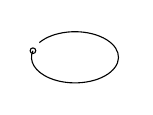
\begin{tikzpicture}[scale=0.65]
\draw (-0.696,0.287) arc (145:-195:0.85 and 0.50);
\draw (-0.821,0.129) circle (0.055);
\end{tikzpicture}
\end{adjustbox}
\end{center}

Слой $F$: $P(z)=\varepsilon$, $\varepsilon$ — мал. компл. число.

Пусть $w_1,w_2,\ldots,w_n$ — набор рац. чисел ($w_i>1$).

\begin{equation*}
z_1^{i_1}z_2^{i_2}\ldots z_n^{i_n};
\qquad \frac{i_1}{w_1}+\frac{i_2}{w_2}+\ldots+\frac{i_n}{w_n}=1.
\end{equation*}

\begin{equation*}
\left(\sum\frac{z_i\frac{\partial}{\partial z_i}}{w_i}P(z)=P(z)\right)
\end{equation*}
[Слева фигурная скобка к подписи:] квазиоднор. полин. $P(z)$.

Тогда гомотопически $F$ — букет сфер $S^{n-1}$ в кол-ве
[Показатель $n-1$ обведён.]
\begin{equation*}
(w_1-1)(w_2-1)\ldots(w_n-1).
\end{equation*}
[Под произведением трёхсторонняя скобка; справа:] (гомотопич. эквив.)

(Оно цело, если изол. особ. точка).

\SourcePage{GELFAND-P000336}{unlabelled}
У преобр. $T$ сосчитан характ. полином

(\underline{Пример:} $z_1^2+\ldots+z_n^2=\varepsilon$. — одна сфера — вещ. котор.
и на неё всё стягивается).

Случай Брискорна:
\begin{equation*}
z_1^{i_1}+\ldots+z_n^{i_n}=\varepsilon.
\end{equation*}

(\underline{И. Бернштейн:} полюса и вычеты $P^\lambda$ связаны с этими целыми.)

\begin{equation*}
H^{n-1}(F)=\mathbb Z^{(w_1-1)\ldots(w_n-1)}.
\end{equation*}

Рассм. групповое кольцо $\mathbb Q(\mathbb C^*)$.
\begin{equation*}
\sum r_i\langle z_i\rangle,\qquad
\langle z_i\rangle\cdot\langle z_j\rangle=\langle z_i z_j\rangle.
\end{equation*}

Вместо $\mathbb C^*$ встр. лишь $\sqrt{1}$, так что
\Unclear{GELFAND-P000336}{group-word}{Короткое сокращение перед $\subset\mathbb C$ имеет а-образное начало, соединённые штрихи с более высоким средним элементом и конечный возврат с точкой; возможны «алг.», «ан.» и «они». Сокращение не раскрыто.}
$\subset\mathbb C$.

\begin{equation*}
\operatorname{div}(t-d_1)\ldots(t-d_k)
=\langle d_1\rangle+\ldots+\langle d_k\rangle
\quad\text{(дивизор).}
\end{equation*}

\underline{Дивизор хар. многочлена $\chi(T)$}
\begin{equation*}
E_k=\frac{\langle1\rangle+\langle\xi\rangle+\ldots+\langle\xi^{k-1}\rangle}{k},
\end{equation*}
\begin{equation*}
\xi=\sqrt[k]{1},\qquad E_k^2=E_k.
\end{equation*}
[Под $\xi=\sqrt[k]{1}$:] первообр.

Пусть $w_i=u_i/v_i$ — несокр.
\begin{equation*}
\operatorname{div}\chi(T)
=(w_1E_{u_1}-1)(w_2E_{u_2}-1)\ldots(w_nE_{u_n}-1).
\end{equation*}

\underline{Получится целый полож. дивизор.}

\underline{\underline{2-я раб.:}} Связь круч. Райдемайстера и $\zeta$-ф-я соотв.
опер. Лапласа на рим. мн-зии.

Зингер и ещё кто-то;
\Incomplete{GELFAND-P000336}{cancelled-bottom}{Зачёркнутая строка после «Зингер и ещё кто-то;» перед «Препринт»: перекрытые буквы и длинные штрихи; текст целиком не восстановлен.}
\underline{Препринт.}

\SourcePage{GELFAND-P000337}{2}
\underline{И. М. Гельфанд.}

\begin{equation*}
\alpha=\begin{pmatrix}A&B\\ C&D\end{pmatrix},
\qquad A,B,C,D\text{ — матрицы.}
\end{equation*}
\begin{equation*}
\det\begin{pmatrix}A&B\\ C&D\end{pmatrix}\text{ — ?}
\end{equation*}

$AD$ нельзя умн., в разн. пр-вах, $AB$, $AC$ не быв. в $\det$.

$A-B\cdot C$. [Справа:] $D$ лишь в середине.

$A-BD^{-1}C$.
\begin{equation*}
\det\alpha=\det[A-BD^{-1}c]\cdot\det D.\qquad(?)
\end{equation*}
\Unclear{GELFAND-P000337}{schur-letter}{В этой строке последняя буква в $BD^{-1}c$ выглядит строчным $c$; в соседних строках стоит прописное $C$. Строчное начертание сохранено.}

\underline{Усл. полож. опред.:} $D\geq0,\quad A-BD^{-1}C\geq0$.

[Ниже повторено:] $A-BD^{-1}C$.

\underline{\underline{С. П. Новиков.}} О \underline{\underline{$\det$}}
\Incomplete{GELFAND-P000337}{cancelled-heading}{Между $\det$ и «(коммут.)» зачёркнуто короткое слово; старые буквы перекрыты и не восстановлены.}
(коммут.).

\begin{equation*}
\begin{array}{ccc}
\mathbb C^n&\overset{A}{\longrightarrow}&\mathbb C^n\\
e_1,\ldots,e_n&&e'_1,\ldots,e'_n
\end{array}
\qquad \det A.
\end{equation*}

\begin{equation*}
\{0\longrightarrow\mathbb C^{n_1}
\overset{A_1}{\longrightarrow}\mathbb C^{n_2}
\overset{A_2}{\longrightarrow}\ldots
\overset{A_{k-1}}{\longrightarrow}\mathbb C^{n_k}_k
\longrightarrow0\}=C.
\end{equation*}
\Unclear{GELFAND-P000337}{chain-last}{У последнего $\mathbb C$ в цепочке сверху $n_k$, снизу отдельное $k$-образное начертание. Нижний знак сохранён как $k$; его роль неясна.}

Классич. $\det$ опред. для точных послед.

Во всех $\mathbb C^{n_i}$ св. базисы $e_1^{(i)},\ldots,e_n^{(i)}$.

(дат. бивектора $e_1^{(i)}\wedge\ldots\wedge e_n^{(i)}$ — эл. объёма).
\Unclear{GELFAND-P000337}{exterior-fullrow}{Кандидат «дат. бивектора», окончание допускает также «бивекторы». Последнее $e_n^{(i)}$ имеет нижнее $n$ без видимого дополнительного $i$; дополнительный индекс не внесён.}

\begin{equation*}
0\longrightarrow\mathbb C^n\overset{A}{\longrightarrow}\mathbb C^n
\longrightarrow0.\qquad\det A.
\end{equation*}
\begin{equation*}
\begin{array}{ccccc}
0\longrightarrow\mathbb C^{n_1}&\overset{A_1}{\longrightarrow}
&\mathbb C^{n_2}&\overset{A_2}{\longrightarrow}&\mathbb C^{n_3}\longrightarrow0\\
e'&&e&&e''
\end{array}
\end{equation*}

Счит. $\det$ перехода от $e$ к $(A_1e',A_2^{-1}e'')$. Это $\det C$.

\SourcePage{GELFAND-P000338}{unlabelled}
\SourceFigure{GELFAND-P000338}{quotient-diagram}{Вверху $\mathbb C^{n_2}$ со стрелкой $A_2$ вправо к $\mathbb C^{n_3}$; от второго объекта стрелка $A_3$ вправо заканчивается без читаемой подписи. Над ней справа объект $\mathbb C^{n_3}/\operatorname{Im}A_2$: к нему поднимается наклонная стрелка, от него спускается стрелка вправо. От верхнего левого объекта стрелка $A_2$ идёт вниз вправо к обведённой дроби $\mathbb C^{n_2}/\mathbb C_{n_1}$, нижний индекс знаменателя плотный и допускает $n_1$ или $n_4$. От обведённого объекта наклонная стрелка поднимается к $\mathbb C^{n_3}$. Ниже слева $0$, от него стрелка поднимается вправо к обведённому объекту; от объекта стрелка опускается вправо к другому $0$. Точное чтение нижнего индекса и всех соединений требует источника.}

[Перед выражением — плотный зачёркнутый знак:]
\Unclear{GELFAND-P000338}{cancelled-product}{Сохранились две вертикали и верхний штрих, похожие на $\prod$, с наложенной чертой; зачёркнутый знак не установлен.}
$(-1)^i\det$ троек
[под словами «$\det$ троек» трёхсторонняя скобка],
не зав. от выб. базисов в пром. пр-вах.

[Два коротких горизонтальных разделительных штриха.]

\underline{Линзовые пр-ва.}
\begin{equation*}
A=\begin{pmatrix}\xi^\alpha&0\\0&\xi^\beta\end{pmatrix},
\qquad \xi=\sqrt[p]{1}.
\end{equation*}
\underline{первообр.}

[В исходном изображении над записью корня — маленький жёлтый значок комментария; его содержимое на кадре не раскрыто.]

[Справа:] Без неподв. точек.

[Справа:] $q=\alpha/\beta$;
\Unclear{GELFAND-P000338}{lens-symbol}{Перед $\alpha/\beta$ знак с петлёй и нижним штрихом: возможны $q$ и $\varphi$. Кандидат $q$ сохранён без установления смысла отношения.}

\underline{\underline{$A_{1,\beta}$.}}

\underline{Фактор сферы} — \underline{линзовое пр-во}.
\begin{equation*}
L_p^3=S^3/A_{1,\beta}.
\end{equation*}
[Справа, отделено двумя вертикальными чертами:] как пр-ва с действ. кон. гр.

Гомеом. они или нет? Гомологии одинаковы.

[Горизонтальная разделительная линия из двух частей.]

$\xi^p=1$. Фунд. гр. линз. мн. — цикл. группа.

Гран.
\begin{equation*}
\begin{array}{cccc}
\sigma^3&\sigma^2&\sigma^1&\sigma^0\\
0&p\sigma^1&0&0
\end{array}
\end{equation*}
[Между строками горизонтальная линия, под ней над каждым членом короткий вертикальный штрих.]
\Unclear{GELFAND-P000338}{lens-boundaries}{Под $\sigma^2$ коэффициент перед $\sigma^1$ имеет $p$-образное начертание; $p$ и $\rho$ графически близки. Кандидат $p\sigma^1$ сохранён.}
— как у проект. пр-ва.

Универс. накр.
\begin{equation*}
\begin{gathered}
\xi\sigma^3\\
\xi^2\sigma^3\\
\ldots
\end{gathered}
\end{equation*}

\underline{Модуль}

\underline{Над групп. кольцом} $\mathbb Z[\pi_1]$, $\pi_1=\mathbb Z_p$.

\SourcePage{GELFAND-P000339}{3}
Комплекс коцепей точен.

$\sigma^3\overset{\partial}{\longrightarrow}$
\Incomplete{GELFAND-P000339}{cancelled-chain}{После первой стрелки перед $(1-\xi^\beta)\sigma^2$ зачёркнуто целое выражение. Видны перекрытые петли, наклонные и длинные горизонтальные штрихи; выражение не восстановлено.}
\begin{equation*}
(1-\xi^\beta)\sigma^2
\end{equation*}
\begin{equation*}
\sigma^2\overset{\partial}{\longrightarrow}
(1+\xi+\ldots+\xi^{p-1})\sigma^1.
\end{equation*}
\Unclear{GELFAND-P000339}{chain-indices}{У $\sigma^2$ в конце первой строки и $\sigma^1$ в конце второй — плотные перечёркнутые нижние знаки, напоминающие $k$; их прежний вид не установлен. Верхний показатель у первой $\xi$ петлистый, кандидат $\beta$.}

$\partial\sigma^1=(1-\xi^{\phantom{1}})\sigma_0$.
\Incomplete{GELFAND-P000339}{cancelled-power}{В показателе $\xi$ внутри $(1-\xi^{\phantom{1}})$ — сплошной тёмный зачёркнутый знак; первоначальный показатель не восстановлен. Пустое место обозначает его позицию.}
[Справа:] точная.

Точная послед.

\underline{Последние — $0$-й оператор.}
\begin{equation*}
\det=(1-\xi)(1-\xi^\beta).
\end{equation*}

\underline{Общее опр.} — чтобы понять инвариантность.

[Под «Общее», соединено вертикальной чертой:] любая фунд. группа.

Предст. такое, чтобы компл. на накрыв. был точным.

\underline{\underline{В. И. Арнольд.}}\qquad $\Lambda=\mathbb C^k$.
\begin{equation*}
A:\Lambda\longrightarrow\operatorname{End}(\mathbb C^n),
\qquad A(0)=A_0.
\end{equation*}
[Под стрелкой:] росток.

Они — категория. Финальный объект — верс. деформ.

$C(\lambda)$ — деф. единицы.
\begin{equation*}
C(\lambda)A(\lambda)(C(\lambda))^{-1}=B(\lambda),
\qquad C(0)=1.
\end{equation*}

$\varphi:M\longrightarrow\Lambda,\quad\varphi^*A$
\Unclear{GELFAND-P000339}{morphism-symbol}{Знак карты и знак перед звёздочкой петлистые, с нижним штрихом; сохранён кандидат $\varphi$, возможен $\psi$. Тот же кандидат в $A(\varphi(\mu))$ ниже}
\Incomplete{GELFAND-P000339}{induced-star}{После $A$ сверху находится небольшой сплошной зачёркнутый знак; его содержание не восстановлено.}
— индуц. деформ.

Версальная деф. $A$ — всякая деф. $B$ матр. $A_0\sim$ индуц.
[Справа ниже дописано: $A$.]
\begin{equation*}
(B(\mu)=C(\mu)A(\varphi(\mu))c^{-1}(\mu)).
\end{equation*}
\Unclear{GELFAND-P000339}{inverse-letter}{В последнем обратном множителе начальная буква открыта снизу, со средней маленькой петлёй: кандидаты строчное $c$ и $e$. Сохранён кандидат $c^{-1}(\mu)$, не заменённый автоматически на $C^{-1}(\mu)$.}

$\exists$ верс. сем. с $9$-ю парам.

\SourceFigure{GELFAND-P000339}{versal-matrix}{Слева прямоугольник, разделённый вертикалью примерно после трёх пятых ширины и горизонталью примерно на середине высоты. В верхнем левом блоке по диагонали три $\lambda$, две $1$ над диагональю; вдоль нижнего края этого блока $\alpha_1,\alpha_2$ и плотное $\lambda+\alpha_3$ у пересечения. Справа на том же уровне $\alpha_4,\alpha_5$. Внизу слева $\alpha_6$ выше и $\alpha_7$ у нижней границы. Нижний правый блок: $\lambda$ и $1$ в верхней строке, $\alpha_8$ и $\lambda+\alpha_9$ в нижней. Некоторые линии проходят через подписи, точные клетки и пересечение около $\alpha_3$ не установлены; незаполненные места не объявлены нулями.}

\underline{$\alpha_i$ — своб. параметры.}

\SourcePage{GELFAND-P000340}{unlabelled}
Разм. пр-ва вариаций:
\begin{equation*}
\sum_\lambda(n_1+3n_2+5n_3+\ldots)
\end{equation*}
\begin{equation*}
n_1(\lambda)\geq n_2(\lambda)\geq\ldots
\end{equation*}

Через $A_0$ провести мн-зие, трансверс. к орбите.

Деформации единицы — $n^2$ парам.

\SourceFigure{GELFAND-P000340}{miniversal-sketch}{Слева прямоугольная схема с широким левым участком и двумя более узкими вертикальными участками справа. В нижней половине два горизонтальных разделения; у левой границы ниже верхнего разделения вертикальная волнистая полоса. Верхняя волнистая горизонтальная полоса идёт слева направо, нижняя различима в средних и правых участках; в нижнем ряду у границы между широким левым и средним участком вертикальная волнистая полоса, внизу справа короткие горизонтальные волнистые штрихи. Подписей нет. Точные клетки, порядок блоков и смысл волн не установлены.}

\Unclear{GELFAND-P000340}{dimension-first-word}{Слово перед тире похоже на «Вазов», «Базов» или «Вызов»; начальная буква и гласная не установлены уверенно.} — подсчёт размерности, пост. вопроса.

Версальность $\Leftrightarrow$ трансверсальность (к орбите) —
— нормаль к орбите.

Нормаль — \Unclear{GELFAND-P000340}{normal-cancelled}{почти; начало слова переписано плотными штрихами, окончание «ти» читается, прежние буквы не установлены}
\underline{централизатор}.

Для квадр. форм. — кан. вид кв. форм.

\SourcePage{GELFAND-P000341}{unlabelled}
[Верхняя часть кадра пустая.]

\underline{15/III}\qquad \underline{\underline{Л. Фаддеев.}}
\begin{equation*}
u_t+2u_{xxx}+6u_xu=0.
\end{equation*}
\Unclear{GELFAND-P000341}{kdv-coefficients}{Перед $u_{xxx}$ видна $2$ с густым старым петлистым штрихом выше; перед $u_xu$ — $6$ с переписанным верхом. Сохранены кандидаты $2$ и $6$, прежние коэффициенты не установлены.}

$u(x,\delta)\longrightarrow0$ при $|x|\longrightarrow\infty$.
\Unclear{GELFAND-P000341}{time-symbol}{Второй аргумент $u$ имеет верхний загнутый штрих и нижнюю петлю, похожие на $\delta$; кандидат $t$ возможен по роли времени. Здесь и ниже в уравнении для $\psi$ сохранено начертание $\delta$.}

[Справа, отделено двумя вертикальными чертами:]
Здесь нет ударных волн. (много $1$-х интегралов).

Рассм. $\psi''+k^2\psi=u(x,\delta)\psi$.

Спец. решение:
\begin{equation*}
\begin{aligned}
\psi|_{x\to-\infty}&=e^{ikx}+a(k)e^{-ikx}\\
\psi|_{x\to+\infty}&=e^{ikx}\cdot b(k).
\end{aligned}
\end{equation*}

Выводится $|a(k)|^2+|b(k)|^2=1$.

\underline{Изв. факт:} $a(k)$ определяет $u(x)$

$u(x)\longleftrightarrow a(k)$ (с точн. до дискр. спектра).

Рецепт: $|a(k,t)|=|a(k)|$

\underline{$\arg a(k,t)=\arg a(k)+Ck^3t$.}

$u(x,t)\longleftrightarrow a(k,t)$.

И с дискр. спектром $A$, $-æ^2$ — это солитоны,
\Unclear{GELFAND-P000341}{eigenvalue}{После $A,$ отрицательное число с показателем $2$; нижняя буква состоит из двух соединённых петель и выглядит как $æ$. Кандидат $-\kappa^2$ возможен по математической роли, но не подставлен вместо видимого $-æ^2$.}
когда $a(k)\equiv0$.
\Unclear{GELFAND-P000341}{final-a}{Буква перед $(k)\equiv0$ плотная, с наложенным штрихом; кандидат $a$ сохранён, раннее начертание не установлено.}

\SourcePage{GELFAND-P000342}{unlabelled}
\underline{Вывод:} похоже на гамильт. ур-е в перем. действие — угол.

$a(k,t)$ — реш. классич. сист. Гамильтона
\begin{equation*}
\begin{cases}
\dfrac{\partial|a|}{\partial t}=0\\
\dfrac{\partial\varphi}{\partial t}=Ck^3.
\end{cases}
\end{equation*}
[Справа от второго уравнения зачёркнутая запись:]
\Unclear{GELFAND-P000342}{phase-full}{В зачёркнутой записи видны $H$-образный знак и маленький $k$-образный нижний штрих; кандидат $H_k$, точное старое выражение не установлено.}

\underline{\underline{Утв.:}} — ур-е — $\infty$-мерное вполне интегр. гамильт.
ур-е. Реш. зад. рассеяния — его канонич. преобр.
к явно решаемому виду.

\underline{Симплектич. структура в пр-ве ф-й $u(x)$.}
\begin{equation*}
\begin{aligned}
\langle u|v\rangle
={}&\int_{-\infty}^{\infty}u(x)\,dx\int_{-\infty}^{x}v(y)\,dy\\
&-\int_{-\infty}^{\infty}v(x)\,dx\int_{-\infty}^{x}u(y)\,dy.
\end{aligned}
\end{equation*}
[Между минусом и вторым интегралом зачёркнуто:]
\Unclear{GELFAND-P000342}{skew-cancelled}{$(u\to v)$ или $(u\leftrightarrow v)$; видны обе буквы, скобки и горизонтальный штрих, направление стрелки перекрыто зачёркиванием.}

невырожд. кососимм. форма.

\underline{Гамильтониан:}
\begin{equation*}
Q(u)=\int_{-\infty}^{\infty}(u^3+u'^2)\,dx
\end{equation*}
\begin{equation*}
\frac{\partial u}{\partial t}=\left(\frac{d}{dx}\right)
\left(\frac{\delta Q}{\delta u(x)}\right).
\end{equation*}

В общ. виде для $(Jx,x)$ и $H(x)$ ур-е
\begin{equation*}
\langle x,y\rangle=(Jx,y);
\end{equation*}
\begin{equation*}
\dot x=J^{-1}\frac{\partial H}{\partial x}.
\end{equation*}
[Под формулой горизонтальная черта с боковыми вертикалями; верхней черты не видно.]
\Unclear{GELFAND-P000342}{general-form}{В вводной строке обе буквы в паре выглядят как $x$: $(Jx,x)$. В следующей строке написано $(Jx,y)$. Различие сохранено, первая пара не исправлена по кососимметрии.}

Или:
\begin{equation*}
\left\langle v\left|\frac{du}{dt}\right.\right\rangle
=(dQ(u))(v).
\end{equation*}
[Под всем равенством трёхсторонняя скобка; справа:] — прав. форма.

В \Unclear{GELFAND-P000342}{classical-path}{Короткое сокращение перед «пучке» похоже на «кокас.»; также сохранены варианты «клас.» и «коас.». Видны начальный к-образный штрих, округлое о и второй к-образный переход; сокращение не раскрыто.}
пучке — $2$ ур-я для $p$ и $q$.

Перейдём от $u$ к $a(k)$.
\begin{equation*}
Q(u)=\int_{-\infty}^{\infty}(u^3+u'^2)\,dx
=\int_{-\infty}^{\infty}\ln(1-|a|^2)k^4\,dk.
\end{equation*}

(Ф-ла следов: Л. Д. Фаддеев и Буслаев,
\Incomplete{GELFAND-P000342}{trace-cancelled}{Между «Буслаев,» и «ДАН» густо зачёркнут маленький знак с остатками петли; первоначальная запись не восстановлена.}
ДАН, 1960 (2)).

\SourcePage{GELFAND-P000343}{6}
Выраж. любой $\int$ такого вида (лок. ф-л) через моменты
логарифма $\ln(1-|a|^2)$.

Образ дифф. формы $\longrightarrow$ в кан. пр-ве (перех. нелинейный).

\begin{equation*}
\langle\delta u_1,\delta u_2\rangle_u
=i\int_{-\infty}^{\infty}\frac{k}{1-|a|^2}
\delta_1a_k(k)\,\delta_2a_k(-k)\,dk=
\end{equation*}
\Unclear{GELFAND-P000343}{twoform-indices-full}{Маленькие нижние знаки после обоих $a$ переписаны, с тёмными петлями; сохранён кандидат $k$ в $a_k(k)$ и $a_k(-k)$, исходные индексы не установлены.}
\begin{equation*}
=\int_{-\infty}^{\infty}
k\delta_1\{\ln(1-|a|^2)\,\delta_2\arg a
\end{equation*}
[Под левой частью дуга с подписью $dp$; под $\delta_2\arg a$ скобка «2-я вар.» и нижняя дуга $dq$.]
\Unclear{GELFAND-P000343}{twoform-row}{Перед $\ln(1-|a|^2)$ видна открывающая фигурная скобка; закрывающая скобка и $dk$ в конце этой строки не видны. Под левой частью дуга с подписью $dp$, под $\delta_2\arg a$ скобка «2-я вар.» и нижняя дуга $dq$. Невидимые завершения не добавлены.}

При налич. соб. знач. — добавки.

\underline{3-мерная обр. задача рассеяния.}
\begin{equation*}
-\Delta\psi+v(\vec x)\psi=k^2\psi,\qquad\vec x\in\mathbb R^3,
\end{equation*}

$v(\vec x)$ дост. быстро убывает при $|\vec x|\longrightarrow\infty$

Амплитуда рассеяния.

Естеств. реш.
\begin{equation*}
\begin{aligned}
\psi(\vec x,\vec k)&=e^{i(\vec k,\vec x)}
+\frac{e^{ikr}}{r}\cdot f\left(\vec k,\frac{\vec x}{r}\right)+\\
&+o(1/r).
\end{aligned}
\end{equation*}
[Под дробью и концом формулы ступенчатая линия; слева ниже: $r\longrightarrow\infty$.]
\Unclear{GELFAND-P000343}{asymptotic}{В конце первой строки после $f$ виден плюс; на следующей строке перед $o(1/r)$ ещё один плюс. Оба сохранены, маленькое $o$ не заменено на $O$.}

$f$ — амплит. рассеяния, ф-я от $5$ перем. (т. к. $\vec x/r$).

Найдены соотн. на амплит. рассеяния, убив. $2$ парам.

[Зачёркнуто:] $f(k)$.
\Unclear{GELFAND-P000343}{cancelled-amplitude}{В зачёркнутом начале строки сохраняются высокое $f$-образное начертание и $(k)$; кандидат $f(k)$, плотное начало не установлено окончательно.}
\begin{equation*}
f\left(k\left|\frac{\vec k}{k},\frac{\vec x}{r}\right.\right)
\longrightarrow f(k|\vec\alpha,\vec\beta)
\end{equation*}

в $L_2(S^2)$ \underline{унит. оператор!} — это условие;

аналог.
\Incomplete{GELFAND-P000343}{cancelled-analogy}{Между «аналог.» и $a^2+b^2=1$ зачёркнуто короткое выражение; перекрытые буквы не восстановлены.}
$a^2+b^2=1$.

$S(k)=I+f$, $f$ — $\mathcal B L_2(S^2)$ если
\Incomplete{GELFAND-P000343}{operator-end}{После «если» перед «опер. с ядром» зачёркнуто слово с наложенными штрихами; слово не восстановлено.}
опер. с ядром.

\SourcePage{GELFAND-P000344}{unlabelled}
\begin{equation*}
S(k)=Q_\gamma^{(+)}\cdot(Q_\gamma^{(-)}(k))^{-1}
\end{equation*}
\Unclear{GELFAND-P000344}{scattering-product}{После $Q_\gamma^{(+)}$ видна точка и длинная наклонная черта у начала следующей скобки. Произведение сохранено как кандидат; роль наклонной черты и возможное прежнее деление не установлены. У первого $Q$ аргумент $k$ не виден.}

где $Q$ Вольтерровские, $\gamma$ — ед. вектор.

[Под $Q$, соединено вертикальной чертой:] по углу $\theta$, отсчит. от $\gamma$.

\begin{equation*}
h_\gamma(k;\alpha,\beta)\Theta[\pm(\alpha-\beta,\gamma)]
=f\left(k\left|\frac{\vec k}{k},\frac{\vec x}{r}\right.\right)
\end{equation*}

При $(\alpha,\gamma)=(\beta,\gamma)$
будет ф-я, аналит. по $k$ в верхней полуплоскости.

Ф-я Грина и факторизация написаны (неск. лет назад).

Не было обр. зад из-за дискр. спектра.

\underline{А. Габриэлов.}

Раб. Гриффитса о периодах рац. интегралов. \underline{Annals of Math.}

\begin{equation*}
\omega=\frac{P(z)}{Q(z)}\,dz_1\wedge\ldots\wedge dz_n,
\qquad P,Q\text{ — многочлены в }\mathbb C^n.
\end{equation*}

$V$ — нули $Q(z)$.

$\Gamma$ — $n$-мерн. циклы в $\mathbb C^n\setminus V$.

$\int_\Gamma\omega$ — периоды.

\underline{1 переменная:} $\omega=\dfrac{P(z)}{Q(z)}\,dz$

$\Gamma$ свод. к станд. набору путей

\begin{center}
\begin{adjustbox}{max width=\linewidth}
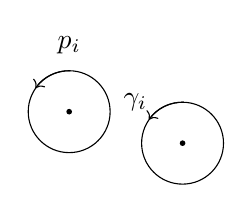
\begin{tikzpicture}[scale=0.8]
\draw (0,0) circle (0.65);
\fill (0,0) circle (0.045);
\draw[->] (0.02,0.65) arc (88:145:0.65);
\node at (0,1.05) {$p_i$};
\node at (1.05,0.15) {$\gamma_i$};
\draw (1.8,-0.5) circle (0.65);
\fill (1.8,-0.5) circle (0.045);
\draw[->] (1.82,0.15) arc (88:145:0.65);
\end{tikzpicture}
\end{adjustbox}
\end{center}

\begin{equation*}
\Gamma=\sum\mu_i\gamma_i;\qquad
\int_\Gamma\omega=\sum\mu_i\int_{\gamma_i}\omega.
\end{equation*}

Свед. к $1$-му пор. — вычитаем полный дифференциал.

И теперь $\sum$ вычетов.

[Горизонтальная разделительная линия из двух частей.]

Счит. форму зад. на $\mathbb{CP}^n$.

$P_n\supset V$ — мн-зие полюсов.

Сущ. $Q$ — однор. форма степени $m$, минимальная.
\SourcePage{GELFAND-P000345}{7}
\begin{equation*}
\Gamma\subset P_n\setminus V,\qquad \Gamma\in H_n(P_n\setminus V,Z).
\end{equation*}
\fbox{Заметим, что $\Gamma$ в $P_n$ есть $0$;}

[Справа:] $n$ — неч. $\Rightarrow H_n=0$.
$n=2k+1\Rightarrow H_n(P_n)=0$.

\underline{$n$ — чётно $=2m$}, $H_n(P_n)=Z$.
% Равенство заходит на закрывающую скобку.

Тогда [зачёркнуто: \Unclear{GELFAND-P000345}{plane-cancel}{неразборчивое слово};
сверху в обводке со стрелкой вставлено: плоское] сечение $P_m$ — единств. образующая.
Дост. сосчитать индекс пересеч. $\Gamma$ с $P_m$.

Рассм. $W=P_{m+1}\cdot V=q\cdot P_m$, $q$ — степень мн., задающего $V$.

Это след. из $W\cdot P_m=V\cdot P_1$ (теор. Безу),
\begin{equation*}
(z_1^2+z_2^2+z_3^2=0\sim 2P_1).
\end{equation*}
\begin{equation*}
0=\Gamma\cdot W=q\Gamma P_m
\quad[\text{зачёркнуто: }\Unclear{GELFAND-P000345}{intersection-cancel}{2?}],
\end{equation*}
отсюда \fbox{$\Gamma P_m=0$}, \underline{что и треб.}

Сущ. цепь $R$ [под $R$ вставлено: в $P_m$], такая что \underline{$\partial R=\Gamma$}.

Счит. $R$ и $V$ в общем положении, $\gamma=R\cdot V$,
$\gamma\in H_{n-1}(V,Z)$.

Возьмём $T_\varepsilon(\gamma)$ — $\varepsilon$-окр. цикла $\gamma$ в $P_n$.
% γ в первом аргументе сильно усилена.
\begin{gather*}
\tau_\varepsilon(\gamma)=\partial T_\varepsilon(\gamma),\\
\partial(R-T_\varepsilon(\Gamma))=\Gamma-\tau_\varepsilon(\gamma).
\end{gather*}
Отсюда $\tau_\varepsilon(\gamma)\sim\Gamma$. Получаем:
\begin{equation*}
\tilde\tau:H_{n-1}(V,Z)\longrightarrow H_n(P_n\setminus V,Z).
\end{equation*}
Это даёт отобр. [зачёркнуто:
\Unclear{GELFAND-P000345}{homology-cancel}{неразборчивое слово}] гомологий.
\begin{gather*}
\tau_\varepsilon(\partial\gamma)=\partial(\tau_\varepsilon(\gamma)),\\
\tilde\tau:H_k(V,Z)\longrightarrow H_{k+1}(P_n\setminus V,Z).
\end{gather*}
\begin{center}— $\cdot$ —\end{center}

\SourcePage{GELFAND-P000346}{unlabelled}
\underline{Арнольд.} Пусть $P_n(x,y)=0$ — плоская неособая ал. кривая.
% Нижняя n в P_n сильно усилена.
\begin{equation*}\underline{n=2k}.\end{equation*}
Теор. Харнака: овалов $\le g+1$, $g=\dfrac{(n-1)(n-2)}2$.

\underline{4-й пор.}
\SourceFigure{GELFAND-P000346}{quartic-ovals}{Четыре овальных контура в два ряда;
верхний правый имеет маленький разрыв, нижний правый — наложенные штрихи.}

\underline{6-й пор.} — 50 случаев (\underline{Гудков}).
Пусть max число овалов 11 (при $n=6$).
\SourceFigure{GELFAND-P000346}{sextic-ovals}{Один большой овал с пятью малыми внутри
и пять малых овалов справа снаружи; верхняя левая часть большого контура имеет небольшой разрыв.}
И ещё 2 случая.

Полож. овалы — леж. в чётном числе других.

Петровский: $|2(p-m)-1|\le 3k^2-3k+1$.
Отсюда не все 11 вне друг друга.

\underline{Гудков:} $p-m\equiv k^2\ (\mathrm{mod}\ 8)$.

\underline{Арнольд и Варченко:} док. mod 4 из-за целочисл. форм.
\begin{equation*}(x,x)=(u,x)\ (\mathrm{mod}\ 2)\end{equation*}
— кв. форма линейна \underline{mod 2}.

\underline{Лемма.} $(u,u)\equiv\operatorname{sgn}(\quad)\ \mathrm{mod}\ 8$.
[Под $(u,u)$: настоящее целое число. Под пустыми скобками со штрихом: кв. формы.]

\underline{Док-во:}
\begin{equation*}(u+2x,u+2x)=u^2+4ux+4x^2,\end{equation*}
а $ux$ и $x^2$ одинак. чётн. по ф-ле.
\begin{center}— $\cdot$ —\end{center}
$z^2=f(x,y)$, $z,x,y$; $(p-m)$ — эйлерова хар. мн-ва меньших знач.

\SourcePage{GELFAND-P000347}{8}
\underline{22/III. А. Габриэлов.}
\begin{equation*}
\int_\Gamma\frac{P(z)}{Q(z)}\,dz_1\wedge\cdots\wedge dz_n,
\qquad\Gamma\text{ — цикл в }P^n\setminus V.
\end{equation*}
$V=\{Q(\xi)=0\}$, $\operatorname{deg} Q=q$.

Цикл $\Gamma$ в $P_n$ гомологичен нулю.
\begin{equation*}\Gamma\in H_n(P_n\setminus V,Z).\end{equation*}
Отобр. $H_n(P_n\setminus V,Z)\to H_n(P_n,Z)$ нулевое.

Пусть $\Gamma\in H_n(P_n\setminus V,Z)$, $n=2m$.
[Перед $V$ в последнем дополнении плотное исправление:
\Unclear{GELFAND-P000347}{complement-overwrite}{прежний знак неразборчив}.]

[Слева:] Инд. пер.
\begin{gather*}
\langle P_m,P_m\rangle=1\text{ — непоср. пров.},\\
\langle P_{m+1}\cdot V,P_m\rangle=q,\\
\langle P_{m+1}\cdot V;P_m\rangle
=\langle V,P_{m+1}\cdot P_m\rangle=V\cdot P_1=q.
\end{gather*}
[Справа под равенством:] (теор. Безу).
\begin{equation*}
0=\Gamma\cdot(P_{m+1}\cdot V)=q(\Gamma,P_m),
\quad\text{отсюда }(\Gamma,P_m)=0.
\end{equation*}
Итак, $\Gamma=\partial R$, $R\cdot V=\gamma\in H_{n-1}(V,Z)$.
% n в последнем индексе сильно усилена.
$T_\varepsilon(\gamma)$ — рассл. на кружочках над $\gamma$.
\begin{gather*}
\partial T_\varepsilon(\gamma)=\tau_\varepsilon(\gamma),\\
\partial(R-T_\varepsilon(\gamma))=\Gamma-\tau_\varepsilon(\gamma).
\end{gather*}
$\tau_\varepsilon(\gamma)$ — канонич. форма цикла $\Gamma$.
[Штрих вниз от $\tau_\varepsilon(\gamma)$ к подписи: рассл. над $\gamma$ на нормальные окружности к $V$.]

Построено отображение:
\begin{equation*}
\tilde\tau:H_k(V,Z)\longrightarrow H_{k+1}(P_n\setminus V,Z),
\qquad\gamma\in H_{n-1}(V,Z).
\end{equation*}
Насколько это неоднозначно?
\begin{equation*}\ker\tilde\tau\big|_{H_k}\text{ — ?}\end{equation*}

\SourcePage{GELFAND-P000348}{unlabelled}
Это кусок точной посл. пары:
\begin{equation*}
H_{n+1}(P_n,Z)\overset{\cdot V}{\longrightarrow}H_{n-1}(V,Z)
\overset{\tilde\tau}{\longrightarrow}H_n(P_n\setminus V,Z)
\overset{0}{\longrightarrow}H_n(P_n,Z).
\end{equation*}
[Зачёркнуто: \Unclear{GELFAND-P000348}{exactness-cancel}{отсюда?}]
Она точна. Обычно mod кручения, но здесь всё хорошо.

[Сверху вставлено: Было док., что] \underline{$\tilde\tau$ эпиморфизм}.
Отсюда точность в том члене.

Из точности: $\ker\tilde\tau$ описывается.
\begin{equation*}
\ker\tilde\tau=H_{n+1}(P_n,Z),\quad
\begin{cases}n\text{ — чётн. — это }0,\\n\text{ — неч. — }Z\text{ с образ. }P_{m+1}.
\end{cases}
\end{equation*}
Точность док-ся станд. способом.

Иначе: пара $P_n$, $P_n$, — трубч. окр. $V$.
Прим. к паре и изом. Тома:
[зачёркнуто: \Unclear{GELFAND-P000348}{thom-cancel}{неразборчивый знак}]
$H_{n-1}\to H_{n+1}$.
% Последняя 1 усилена поверх штрихов.

Док-во точности: Пусть $\tau(\gamma)=\partial R$, $\partial(T(\gamma)-R)=0$
и отсюда $T(\gamma)-R$ — гр. чего-то, пересеч. с $V$ и как раз $\gamma$.
[Перед последним $R$ зачёркнуто:
\Unclear{GELFAND-P000348}{cycle-gamma}{неразборчивый знак}.]

[На левом поле:]
\begin{equation*}
\Gamma\cdot V=\gamma=\partial R';
\end{equation*}
\begin{gather*}
\partial T(R)=\tau(R)+T(\gamma);\\
\Gamma-\partial T(R)=(\underline{\Gamma}-T(\gamma))-\underline{\tau(R)}.
\end{gather*}

Пусть на $P_n$ есть рац. дифф. форма. В однородных коорд.
\begin{equation*}
\mathrm C^{n+1}\setminus\{0\}\underset{\Unclear{GELFAND-P000348}{projection-label}{\pi?}}{\longrightarrow}P_n.
\end{equation*}
Индуц. форма
\begin{equation*}
\Omega=\sum(-1)^j\xi_j\,d\xi_0\cdots\widehat{d\xi_j}\cdots d\xi_n.
\end{equation*}
[Мелкие прежние знаки над $\xi_j$, после $d\xi_0$, у $d\xi_j$ и над последним $d\xi_n$:
\Unclear{GELFAND-P000348}{omega-overwrites}{неразборчивые зачёркнутые индексы}.]
\begin{equation*}
\frac{P(\xi)}{Q(\xi)}\Omega,\qquad
\fbox{$\operatorname{deg} P(\xi)=\operatorname{deg} Q(\xi)-(n+1)$},
\end{equation*}
тогда форма опр. на $P_n$.
\begin{multline*}
\varphi=\frac1{B(\xi)}\left\{\sum_j(-1)^{|j|}
\left[\sum_{\alpha=1}^{\ell}(-1)^\alpha\xi_{j_\alpha}
A_{j_1\cdots\widehat{j_\alpha}\cdots j_\ell}(\xi)\right]\right.\\
\left.(d\xi_0\wedge\cdots\widehat{d\xi_{j_1}}\cdots
\wedge\widehat{d\xi_{j_\ell}}\wedge\cdots\wedge d\xi_n)\right\};
\qquad\operatorname{deg} B=\operatorname{deg} A+(n+2-\ell).
\end{multline*}

\SourcePage{GELFAND-P000349}{9}
Всё неособое.

Это вид форм, являющихся поднятиям с $P_n$.
% Конец «поднятиям» усилен.
\begin{equation*}\frac{P(\xi)}{Q^\ell(\xi)}\Omega.\end{equation*}
Понижаем пор. полюсов вычитанием кограниц.
\begin{multline*}
\frac1{Q(\xi)^\ell}\left\{\sum_{i<j}(-1)^{i+j}
[\xi_i A_j(\xi)-\xi_j A_i(\xi)]\right.\\
\left.(d\xi_0\wedge\cdots\wedge\widehat{d\xi_i}\wedge\cdots
\wedge\widehat{d\xi_j}\cdots\wedge d\xi_n)\right\}.
\end{multline*}
\begin{gather*}
P=\ell\left(\sum A_j\frac{\partial Q}{\partial\xi_j}\right)
-Q\left(\sum\frac{\partial A_j}{\partial\xi_j}\right),\\
\operatorname{deg} P(\xi)=\operatorname{deg} Q(\xi)-(n+1).
\end{gather*}
Annals, v. 90, n. 3, 1969.

\underline{Паламодов.}
\underline{О хар-ках систем лин. ур-й.}
\begin{equation*}
\left\{\begin{aligned}a_1u&=f_1\\&\vdots\\a_tu&=f_t\end{aligned}\right.
\qquad a_1,\ldots,a_t\text{ — дифф. операторы}.
\end{equation*}
[Слева от скобки: система.]

\underline{Пример.}
\begin{equation*}
\begin{cases}D_xu=f,\\(D_y+\lambda)u=g.\end{cases}
\qquad\underline{\text{гл. часть — ?}}
\end{equation*}
Не $\begin{pmatrix}D_x\\D_y\end{pmatrix}$, т.к. следствие системы:
$u=h=D_yg-D_xf$.

Надо выписать все следствия и с ними иметь дело.
\begin{center}— $\cdot$ —\end{center}
Хар-ка — ? $D_xu+D_yv=f$.

Теор. Холмгрена не действ. ни по какому напр., а теор.
\textbf{Коши-Ковал.} по любому.

\SourcePage{GELFAND-P000350}{unlabelled}
\underline{29/III. Ролевич.}
\underline{$A$ — лин. оператор в кон-мерном пр-ве.}

$\{x,Ax,A^2x,\ldots\}$ — замыкание.

\underline{Пред. точки:} $0$, $+\infty$ либо
[зачёркнуто: \Incomplete{GELFAND-P000350}{limit-cancel}{Целое зачёркнутое слово между «либо» и «комп. мн-во» не прочитано.}]
комп. мн-во, не содерж. нуля.

\underline{Пусть опр. в гильбертовом пр-ве, $\ell^p$ или $c^0$.}
Может быть всюду плотным. — сдвиг с умножением.
\begin{equation*}
S(x_1,\ldots,x_n,\ldots)=(x_2,\ldots,x_n,\ldots).
\end{equation*}
\fbox{$A=aS$}, \underline{$a>1$}.
\begin{equation*}
x^{(n)}=\{x_1^{(n)},\ldots,x_{k_n}^{(n)},0,0,\ldots\}
\text{ — лин. мн-во},\quad n=1,2,\ldots.
\end{equation*}
[Под ненулевым блоком со скобкой: рац. числа.]
\begin{equation*}
x=\left\{x^1,0,0,\ldots,0,\frac{x^2}{a^{\alpha_1}},0,\ldots,0,
\frac{x^3}{a^{\alpha_2}},\ldots\right\}.
\end{equation*}
[Под первым промежутком нулей: большое кол-во нулей —
\Unclear{GELFAND-P000350}{zeros-annotation}{счит.?}. Под $a^{\alpha_1}$ короткая дуга.]
\begin{equation*}
x^{(1)}=(x_1^{(1)},x_2^{(1)},\ldots,x_{k_1}^{(1)}).
\end{equation*}
\underline{Топ. эквив. лин. опер.:} $\exists$ гомеом. $U$: $A=UBU^{-1}$.

[Зачёркнуто: \Unclear{GELFAND-P000350}{existence-cancel}{неразборчивое слово};
сверху вставлено: Сущ.] опер. не экв. — плотность орбиты — топ. св-во.

\Incomplete{GELFAND-P000350}{cancelled-line}{Целая строка между «топ. св-во» и «Можно постр.»
перечёркнута горизонталями и петлями; её исходное содержание не прочитано.}

Можно постр. опер., неогр. в $\forall$ норме.

\underline{Арнольд.}
\underline{Милнор} — теория унимод. квадр. целочисл. форм.
\begin{equation*}\varphi:Z^n\times Z^n\longrightarrow Z.\end{equation*}
Унимод.: $\tilde\varphi:Z^n\to Z^{n*}$ изоморфизм.

\underline{Инварианты:} $r$ — ранг; $\operatorname{sgn}$ — сигнатура;
тип, I, II.

Если форма не знакоопред., то сист. полна.

Рассм. квадр. форму $\hat\varphi_2:Z_2^n\to Z_2$, привед. mod 2.
\underline{Она линейна.} Запишем её в виде [зачёркнуто: $(u,x)$;
снизу вставлено:] $\varphi(u,x)=\varphi(x,x)$.

\SourcePage{GELFAND-P000351}{10}
Или $\varphi(x,x)\equiv\varphi(u,x)\ \mathrm{mod}\ 2\quad\forall x$.

Тип I — $\exists$ эл., квадр. к-рого нечётен.

\underline{Лемма:} 1) $\varphi(u,u)\ \mathrm{mod}\ 8$ не зав. от $u$.
($u$ опр. mod $2Z^n$).

2) $\varphi(u,u)\equiv\operatorname{sgn}\varphi\ \mathrm{mod}\ 8$.

(Из $\int$-а Френеля).

\underline{Классиф.:} Не знакоопр.
\begin{gather*}
\text{нечётн.}\quad\sum x_i^2-\sum y_i^2
\quad[\text{зачёркнуто: }\Unclear{GELFAND-P000351}{odd-cancel}{неразборчивый член}],\\
\text{чётн.}\quad kU\oplus\ell\Gamma_8,\qquad
\Gamma_8\text{ — форма Золотарёва, связ. с }E_8,\\
U=\begin{pmatrix}0&1\\1&0\end{pmatrix}.
\end{gather*}
[Справа две параллельные черты и подпись: из K-теории.]

\underline{Полож. опр.} — конечное число в $\forall$ размерности.

\underline{Серр} — учебник \underline{арифметики}.

Стабильно только \underline{ранг} и сигнатура.

[Две стрелки вниз от «ранг» и «сигнатура» к крупной строке:]
Дорогой Миша ты ошибаешься.

\SourcePage{GELFAND-P000352}{12}
\underline{5/IV. Кириллов. Представление по Геронимусу.}
% Окончание «Представление» усилено.
Основано на понятии топологии Гротендика («Топо»).

$C$ — категория, $\forall A\in C$ указаны покрытия
$\{U_\alpha\overset{\varphi_\alpha}{\longrightarrow}A\}$.
% Начальная φ_α усилена.

\underline{Аксиомы:}
\begin{equation*}
1)\quad\{U_{A_\alpha}\overset{\varphi_\alpha}{\longrightarrow}U_\alpha\}
\Longrightarrow\{U_{\beta_\alpha}\overset{\varphi_\alpha\circ\varphi_{\beta_\alpha}}{\longrightarrow}A\}.
\end{equation*}
[Под первой скобкой: покрытия $\forall\alpha$; под второй: покрытие.]
\begin{equation*}
2)\quad\{U_\alpha\times_A B\overset{\varphi_\alpha\times_A1}{\longrightarrow}A\times_A B\}
\quad\text{тоже покрытие}.
\end{equation*}
[Над $1$ отдельно написано $B$ со штрихами вниз.]
При этом зад. морфизм $B\overset{\varphi}{\longrightarrow}A$.

\underline{Опр.} $X_0=B\times_A C$.
\begin{center}
\begin{adjustbox}{max width=\linewidth}
\begin{tikzcd}[column sep=small]
B\arrow[d]&C\arrow[d]\\A&A
\end{tikzcd}
\end{adjustbox}
\qquad
\begin{adjustbox}{max width=\linewidth}
\begin{tikzcd}[column sep=small,row sep=small]
&X_0\arrow[dl]\arrow[dr]&\\B\arrow[dr]&&C\arrow[dl]\\&A&
\end{tikzcd}
\end{adjustbox}
\end{center}
Универс. объект, т.е. $\forall X$,
\begin{center}
\begin{adjustbox}{max width=\linewidth}
\begin{tikzcd}[column sep=small,row sep=small]
X\arrow[r]\arrow[dr]&B\\&C
\end{tikzcd}
\end{adjustbox}
\end{center}
сущ. ед. морфизм
\begin{center}
\begin{adjustbox}{max width=\linewidth}
\begin{tikzcd}[column sep=small,row sep=small]
&X\arrow[d]\arrow[ddl]\arrow[ddr,bend left=15]&\\
&X_0\arrow[dl]\arrow[dr]&\\
B\arrow[dr]&&C\arrow[dl]\\
&A&
\end{tikzcd}
\end{adjustbox}
\end{center}
\Unclear{GELFAND-P000352}{axiom-three-number}{3 или 8}) $U\to U$ покрытие.

(См. Мамфорд.)

\underline{Пучок} — функтор $F:C\overset{\text{контравар.}}{\longrightarrow}K$ — другая категория.
И вып. акс. пучка.
$U_\alpha\overset{\varphi_\alpha}{\longrightarrow}A$.

\SourceFigure{GELFAND-P000352}{sheaf-arrow-label}{Схема $0\to F(A)\to\prod F(U_\alpha)$
с двумя стрелками вправо к $\prod F(U_{\alpha\beta})$.
Первая стрелка от $F(A)$ плотно усилена и подписана $F(\varphi_\alpha)$; под её штрихами слева виден остаток наконечника, обращённого влево, при ясном правом наконечнике; последовательность правки не установлена;
две следующие подписаны $F(\varphi_\alpha)$ и $F(\varphi_\beta)$,
после нижней подписи плотный звёздочкообразный знак с неясным значением.}
[Под $F(A)$ две черты; под $\prod F(U_\alpha)$ скобка.
Ниже:] \underline{$A$ — произв. объект.}

Если образы совпад., то
\begin{equation*}A\longleftarrow U_\alpha\longleftarrow U_\alpha\times U_\beta.\end{equation*}
\underline{Полутоп. есть всюду}.

\SourcePage{GELFAND-P000353}{unlabelled}
$\mathcal U=\{U_\alpha\to A\}$. Когомологии $H(\mathcal U,F)$ (Чеха).

\underline{Нетрив. теорема.} (!) По предыдущему можно постр. пучок.

\Incomplete{GELFAND-P000353}{cancelled-heading}{Плотно зачёркнутый заголовок слева от
«по группе» не прочитан полностью; кандидат «Представления» остаётся неуверенным.}
По группе $G$ стр. «Топо».
А по предст. — пучок над этим «топо».

Идея Геронимуса — когомологии и их связь со стар. предст.

$G$ — группа (Ли). $C$ — это $G$-многообразия.
Морфизмы — $G$-отображения и притом \underline{регулярные},
т.е. $\forall$ точке $M$ [зачёркнуто:
\Unclear{GELFAND-P000353}{tangent-cancel}{неразборчивый знак}] кас. отобр. — эпиморфизм.
[Под $M$: $M\to N$.]

\underline{2-й прим.}
$G$ — кон. гр. — катег. — любые $G$-мн-ва. (Конечные).
% Последние буквы «катег.» усилены.
Кат. $K$ — категория лин. пр-в.
Пучки $\leftrightarrow$ представления.
Пусть зад. предст. $T_g$ в $E$.

[Зачёркнуто: Предст. $\longrightarrow$
\Incomplete{GELFAND-P000353}{cancelled-representation-row}{Правое зачёркнутое слово после «Предст.» и стрелки не прочитано.}.]

Если $X$ — $G$-пр-во [снизу вставлено: из 5 точек], то надо рассм. отобр. $X$ в $E$,
перест. с действием $G$.
\begin{equation*}\xi_{g(i)}=T_g\xi_i.\end{equation*}
Пятёрки — лин. пр-во.
\begin{center}— $\cdot$ —\end{center}
По $X$ и $T_g$ стр. пр-во из ф-й $\xi(x)$.
\begin{equation*}
T_g\xi(xg^{-1})=\xi(x),\qquad\xi(x)\in E.
\end{equation*}
% -1 усилено; остаётся разборчивым.
Есть пучки, к-рые не получ. из представлений.

Теор. элементарных частиц [зачёркнуто:
\Unclear{GELFAND-P000353}{particle-cancel}{ещё / ещ. / другое неразборчивое слово}] не постр.,
т.к. не все предст. известны.
(Ср. спиноры и электроны.)
(Для конеч. группы всякое получ. отсюда).

Иногда получ. когом. топ. пр-ва и когом. как у Гельфанда-Фукса.

\SourcePage{GELFAND-P000354}{13}
\underline{И.М. Гельфанд о гипотезе Вейля.}
\begin{equation*}Q:\quad y^3=x^3-g_1x-g_2.\end{equation*}
$g_1,g_2$ — рац. числа. — элл. кривая $T$.
Над компл. числами.

Есть дискр. группа матриц
$\begin{pmatrix}\alpha&\beta\\A\gamma&\delta\end{pmatrix}$,
$\alpha,\beta,\gamma,\delta$ — целые, $\det=1$.

$A\in Z$, [зачёркнуто:
\Unclear{GELFAND-P000354}{choice-cancel}{неразборчивое слово}] будут выбр.
Груп. mod $A$.

Они опр. дробно-лин. преобр. верхн. полупл. в себя.
\begin{equation*}z'=\frac{\alpha z+A\gamma}{\beta z+\delta}.\end{equation*}
Фунд. область — модулярное мн-зие $X_A$.

Группа $\Gamma_0(A)=\begin{pmatrix}\alpha&\beta\\A\gamma&\delta\end{pmatrix}$.
\SourceFigure{GELFAND-P000354}{fundamental-region}{Под группой — четыре дугообразных
контура над почти горизонтальной линией, две крайние ветви идут вверх;
у первой внутренней ножки маленькая петля, которую нельзя уверенно прочитать как метку.}

[Справа, под $X_A$, рисунок с подписью $A=1$:]
\begin{center}
\begin{adjustbox}{max width=\linewidth}
\begin{tikzpicture}
\draw (0,1.4) .. controls (0.25,1.1) and (0.4,0.35) .. (0.45,0);
\draw (0.45,0) .. controls (0.8,0.35) and (1.25,0.35) .. (1.6,0);
\draw (1.6,0) .. controls (1.55,0.65) and (2.0,1.35) .. (2.65,1.65);
\node at (2.95,0.75) {$A=1$};
\end{tikzpicture}
\end{adjustbox}
\end{center}

Гипотеза Вейля — $\exists$ [над строкой в обводке вставлено: нетрив.] анал. отобр.
$\varphi:X_A\to T$.
(Отображений конечное число; $\forall$ кривой на тор).

\fbox{$p\ne2,3$}.

\underline{Заменим $T$ mod $p$}. Получ. кривая над $F_p$. Она
[плотно усилено/зачёркнуто:
\Unclear{GELFAND-P000354}{singular-cancel}{он?}] может стать особой.
(Т.е. частн. производ. mod $p$ равны $0$).

1) Без особ. точек.

2) Особ. точки с различными касательными.

2а — веществ. [зачёркнуто:
\Incomplete{GELFAND-P000354}{real-tangent-cancel}{Целое зачёркнутое слово между «веществ.» и «касат.» не прочитано.}] касат.

2б — мнимые касательные.

3) Касат. совпадают.
\begin{equation*}
\begin{array}{lll}
A_p=1&p&1\text{ типа}\\
A_p=p&p&2\text{ типа}\\
A_p=p^2&p&3\text{ типа}
\end{array}
\end{equation*}
\SourcePage{GELFAND-P000355}{unlabelled}

$A=\prod_p A_p$ — кондуктор кривой.
\begin{equation*}
L_p(\zeta)=(1-c_pp^{-s}+p^{1-2s})^{-1},\qquad p\text{ — 1-го типа.}
\end{equation*}
\Unclear{GELFAND-P000355}{first-factor-argument}{Первый аргумент — ζ-подобный знак; кандидат ζ, возможно ξ, тогда как далее написано s.}

[Зачёркнуто перед знаком «+»:]
\Incomplete{GELFAND-P000355}{cancelled-count}{Зачёркнутый начальный знак или короткая запись целиком не прочитаны.}
$+$ число точек кривой: $1-c_p+p$.
\begin{equation*}
L_p(s)=(1-\varepsilon_pp^{-s})^{-1},\qquad \text{случай 2)};\qquad
\begin{array}{ll}
\varepsilon_p=+1&2\text{а},\\
\varepsilon_p=-1&2\text{б}.
\end{array}
\end{equation*}
$L_p(s)=1$, случ. 3.
\begin{equation*}
\zeta(s)=\prod_p L_p(s).
\end{equation*}
Разл. $\zeta(s)$ в ряд:
\begin{equation*}
\zeta(s)=\sum_1^\infty\frac{c_n}{n_s}.
\end{equation*}
\Unclear{GELFAND-P000355}{dirichlet-denominator}{В знаменателе s написано снизу: кандидат $n_s$, без исправления на n в степени s.}
Рассм. теперь
\begin{equation*}
\sum_z c_ne^{inz}=\omega(z).
\end{equation*}
\Unclear{GELFAND-P000355}{fourier-index}{Нижний знак суммы похож на z, при $c_n$ и inz.}
Утверждение: $\int\omega(z)\,dz$ — \underline{искомая ф-я}.
Она стр. в верхн. полуплоскости. (и аналит.)
\Unclear{GELFAND-P000355}{primitive-word}{Кандидат сокращения «стр.», возможно «опр.»; перед «верхн.» переписанные или перечёркнутые штрихи, прежний префикс не разделяется уверенно.}
Отобр. верхн. полупл. в компл. прямую.

Гипотеза Вейля: \underline{I.} $\exists$ решётка $\Gamma\subset C^1$, что $\forall g\in\Gamma_0(A)$
\begin{equation*}
\int_z^{gz}\omega(z)\,dz\in\Gamma.
\end{equation*}
[Внизу слева зачёркнут короткий фрагмент:]
\Incomplete{GELFAND-P000355}{cancelled-left}{Короткая зачёркнутая запись на левом поле внизу целиком не восстановлена.}
[Зачёркнутая строка внизу:]
\Unclear{GELFAND-P000355}{cancelled-bottom-word}{Кандидат «отсюда все»; окончание и возможные точки ё закрыты зачёркиванием.}
[Выше продолжения этой строки зачёркнуто:]
\Unclear{GELFAND-P000355}{cancelled-bottom-map}{Кандидат $\Gamma_0(A)\to\Gamma$; аргумент в скобках переписан.}

\SourcePage{GELFAND-P000356}{14}

12/$\overline{\mathrm{IV}}$. \underline{\underline{Переломов.}}

$V$ — $2N$-мерное вещ. пр-во, $B$ — кососимм. билин. форма на $V$.
[Над характеристикой $B$ вставлено и обведено: невыр.]
$B$-решётка $L\subset V$,
\Incomplete{GELFAND-P000356}{cancelled-lattice}{Между включением L в V и следующим тире целиком не прочитан зачёркнутый короткий фрагмент.}
— на $L$ $B$ прин. целочисл. знач.
$J^2=-1$, $J$ согласован с $B$: $J^TBJ=B$.
[Зачёркнута строка: кандидат $v_0$ фикс. вектор; далее тире, запятая и длинный горизонтальный штрих.]
\Unclear{GELFAND-P000356}{cancelled-vector}{В зачёркнутой строке кандидат $v_0$ фикс. вектор; сокращение «фикс.» неуверенное, его средние штрихи пересекаются зачёркиванием. Далее тире, запятая и длинный горизонтальный штрих.}

\underline{Гельфанд о кн. Паули}:
\begin{equation*}
P^2=P,\qquad\lambda^2=\lambda,\qquad\lambda=0,+1,-1.
\end{equation*}
\underline{$-1$} отбрас. из физ. сообр.
\Unclear{GELFAND-P000356}{projector-row}{Написаны P²=P, λ²=λ и одновременно λ=0,+1,−1; всё сохранено вместе со строкой об отбрасывании −1.}
Объём фунд. пар-ма $=1$. (гл. решётка).
Пусть $BJ>0$.
\Unclear{GELFAND-P000356}{b-positive-sign}{Знак сравнения сильно переписан: кандидаты BJ больше 0 и BJ больше или равно 0.}
В $V$ компл. структура. $z\in C^N$.
\begin{equation*}
H(z,z')=B(z,Jz')+iB(z,z')\text{ — эрмитова форма.}
\end{equation*}
[Между знаком равенства и нынешним $B(z,Jz')$ зачёркнута прежняя запись:]
\Incomplete{GELFAND-P000356}{hermitian-cancelled}{Прежняя формула с B-подобным началом закрыта многократным зачёркиванием; её аргументы и знаки не прочитаны.}
Рассм. ф-ю $F$: — целочисленную.
\begin{equation*}
F(\alpha+\beta)\equiv F(\alpha)+F(\beta)+B(\alpha,\beta)\quad(\mathrm{mod}\ 2).
\end{equation*}
К $F$ можно доб. лин. форму.
Выб. базис в $L$.
\begin{equation*}
v\in L\mapsto\kappa_1,\ldots,\kappa_N,\ell_1,\ldots,\ell_N.
\end{equation*}
Считаем:
\begin{equation*}
B=\begin{pmatrix}0&I\\-I&0\end{pmatrix}.
\end{equation*}
[Перед следующей формулой зачёркнут короткий фрагмент:]
\Incomplete{GELFAND-P000356}{cancelled-sum}{Зачёркнутое короткое слово перед F(α) не прочитано целиком.}
\begin{equation*}
F(\alpha)=\sum\kappa_i\ell_i+\sum\varepsilon_i\kappa_i+\sum\tilde\varepsilon_i'\ell_i
\qquad(\text{сущ. }4^N\text{ решений}).
\end{equation*}
\Unclear{GELFAND-P000356}{refinement-prime}{У последнего коэффициента с тильдой отдельный наклонный верхний штрих: кандидат дополнительный верхний штрих у $\varepsilon_i$, без удаления по математическому контексту.}
$\Theta$-ф-я — реш. ур-я
\begin{equation*}
\Theta(z+\alpha)=(-1)^{F(\alpha)}e^{\frac\pi2H(\alpha,\alpha)+\pi H(\alpha,z)}\Theta(z).
\end{equation*}
\Unclear{GELFAND-P000356}{theta-quasiperiod-argument}{Нынешний аргумент H(α,z) с z без отдельной верхней черты; под z остаются перекрытые нижние штрихи прежней записи, не отделённые в уверенный знак.}
[Формула подчёркнута с боковыми штрихами.] (целая ф-я).
Сущ. только одно реш. функц. ур-я с точн. до \underline{\underline{const}}.
(Важно, что решётка главная — $\det B=1$).
Это напис. у Картье (хотя изв. до него).

\SourcePage{GELFAND-P000357}{unlabelled}

\underline{\underline{Физич. задача}} (см. фон Нейман).
Пусть $a$ — опер. уничт., $a|\alpha\rangle=\alpha|\alpha\rangle$ — соб. векторы.
[Справа:] $e^{-\frac{(x-\lambda)^2}{2}}$.
Спектр — вся компл. плоскость.
Сист. сверхполная.
\underline{Зад.}: выделить полную систему.
[Зачёркнуто:]
\Unclear{GELFAND-P000357}{cancelled-reasonable}{Начало «Разумн-», кандидаты «Разумная» и «Разумность»; окончание перекрыто линией.}
Сверхполная — если выбрас. $\forall$ кон. числа ост. полную систему.
(если $\lambda$ им. точку сгущения, то …)
Для какой послед. $\lambda_n$ это полная сист.?
Пусть $\lambda$ — решётка на компл. плоскости $C$.
\begin{equation*}
\begin{array}{ll}
\text{площ. ячейки}>\pi&\text{— неполна},\\
\text{— ″ —}<\pi&\text{— сверхполна}.
\end{array}
\end{equation*}
Пусть площ. ячейки $=\pi$.
выб. 1 точку — полна [вся строка волнисто подчёркнута].
\underline{\underline{выб. 2 точки — неполна}}.
\Unclear{GELFAND-P000357}{overwritten-select}{Перед 2 точки буквы сокращения сильно переписаны: кандидаты «выб.» и «выбр.»; после б видны отдельная петля и нисходящий р-подобный штрих. Прежние штрихи не разделены уверенно; сокращение не развёрнуто.}
Т.е. есть в точности 1 соотношение.
\begin{equation*}
f(z)=\sum(-1)^{mn+m+n}e^{-\frac12|\lambda_{mn}|^2+\lambda_{mn}z}=0.
\end{equation*}
\Unclear{GELFAND-P000357}{identity-first-z}{В конце показателя кандидат z с поперечной чертой внутри буквы; отдельная верхняя черта не видна.}
$\lambda_{mn}=m\omega_1+n\omega_2$.
(уже в $F_2$) — всё делится.
или
\begin{equation*}
\sum(-1)^{mn+m+n}e^{-\frac{(x-\lambda_{mn})^2}{2}}.
\end{equation*}
[Первая пара букв показателя знака утолщена.]
\begin{equation*}
|\langle\alpha|\beta\rangle|^2=e^{-|\alpha-\beta|^2}.
\end{equation*}
(\underline{Нейман} и \underline{Шенберг} — полож. опр. ф-и).
\underline{Вопрос фон Неймана}:
рассм. решётку с пл. $\pi$ и ф-и $|\alpha_{mn}\rangle$.
В этих сост. опр. дисперсии $X$ и $p$.
$\delta_x\cdot\delta_p$ растёт для ортогон. сист. обычно.

\SourcePage{GELFAND-P000358}{15}

\underline{\underline{Вопр. фон Неймана.}}
Будет ли $\delta_x\cdot\delta_p$ после ортогонализации этих векторов
ограничено на этой системе?
Гельф. счит., что это маловероятно.
Неясен общ. \underline{вопр.} для \underline{ортог. сист.}
[Две строки зачёркнуты горизонтальными и многократными косыми штрихами; читаются фрагменты: Переломов умеет док-ть это для ортог. решётки … (из тожд. Якоби $(z=0)$).]
\Incomplete{GELFAND-P000358}{cancelled-two-lines}{В двух зачёркнутых строках конец первой и начало второй строк, включая часть скобки, не восстановлены; сохранены читаемые фрагменты.}
[На левом поле:] $\pi$.
Общ. тожд. \underline{не выв.} из \underline{тожд.} Якоби.
\Unclear{GELFAND-P000358}{from-rewrite}{Предлог «из» переписан тёмными штрихами; нынешний кандидат «из», прежняя запись не отделяется уверенно.}
Это переносится на $N$-мерный случай.
Получ. $2^{N-1}(2^N-1)$ тождеств.
Итак, элем. задача:
\begin{equation*}
\sum(-1)^{mn+n+m}e^{-\frac12|\lambda_{mn}|^2+\lambda_{mn}z}=0,
\end{equation*}
\Unclear{GELFAND-P000358}{identity-final-z}{В конце показателя кандидат z без отдельной верхней черты; верхний штрих относится к самой перечёркнутой букве z.}
если площ. решётки $=\pi$.
\underline{Док-во}: рассм. гильб. пр-во с
\begin{equation*}
\int\bar f(z)g(z)e^{-|z|^2}\,dz\,d\bar z.
\end{equation*}
[На левом поле, первый знак утолщён:] $|\lambda_{mn}\rangle$.
Рассм. $|\lambda\rangle$ и $|\psi\rangle\in\mathcal H$.
\begin{equation*}
\langle\psi|\lambda\rangle=e^{-\frac{|\lambda|^2}{2}}\underline{\psi(\lambda)}.
\end{equation*}
[Под подчёркнутым выражением:] целая аналитич.
\underline{Ортог.}
\begin{equation*}
\langle\psi|\lambda_{mn}\rangle=e^{-\frac{|\lambda|^2}{2}}\psi(\lambda_{mn}).
\end{equation*}
\Unclear{GELFAND-P000358}{norm-denominator}{В норме второй формулы написано λ без mn, хотя в кет-векторе и аргументе ψ стоят $\lambda_{mn}$.}
\underline{Целая с 0-ми в зад. мн-ве точек.}
Надо док., что её не сущ. в $F_2$.
(см. Левин, \underline{станд.} \underline{теорема}).
[Внизу перед G зачёркнут отдельный знак:]
\Incomplete{GELFAND-P000358}{cancelled-matrix-prefix}{Изолированный зачёркнутый знак перед G целиком не восстановлен.}
\begin{equation*}
G=\begin{pmatrix}1&\alpha&\delta\\0&1&\beta\\0&0&1\end{pmatrix},
\qquad\Gamma=\begin{pmatrix}1&\alpha&k\pi\\0&1&\beta\\0&0&1\end{pmatrix}.
\end{equation*}
$\alpha,\beta,\delta$ — веществ.
$\alpha+i\beta\in L$.
[Под $L$, с коротким вертикальным штрихом:]
\underline{Наша}\newline\underline{решётка.}
$K$ — целое.
\SourceFigure{GELFAND-P000358}{lattice-caption-geometry}{В правой нижней матрице α и β сильно переписаны; верхний правый элемент имеет k-подобный знак перед π. Справа α+iβ принадлежит L, под L короткая вертикальная черта к подчёркнутым словам «Наша решётка». Ниже матрицы написано K — целое. Прежние штрихи матрицы и точное соединение подписи оставлены для проверки по источнику.}

\SourcePage{GELFAND-P000359}{unlabelled}

Рассм. операторы.
\begin{equation*}
\underline{D=e^{i\varphi}e^{i(\alpha^*a-\alpha a^*)}}\text{ — 3-парам. группа.}
\end{equation*}
алг. Ли — $a,a^+$ и $1$; $[a,a^+]=1$, ост. коммут. $0$.
$\Gamma$ — $\alpha$-точки решётки; $\varphi$ — $0$ и $\pi$.
Тогда предст., индуцир. представл. $(-1)^{mn+m+n}$ дискр. гр. $\Gamma$ неприводимо.
\underline{Есть перенос на произв. группу}.
[На левом поле, подчёркнуто:]
\Unclear{GELFAND-P000359}{margin-name}{Кандидат «Каждан.»; средние штрихи сжаты, возможен буквальный вариант «Камдан.».}
$G$ — полупр. группа, $T$ — её предст. в $H$.
\Unclear{GELFAND-P000359}{group-word}{Сокращение после G —: кандидаты «полупр.» и «полугр.»; сжатые буквы не позволяют уверенно разделить.}
[Над $H$ обведено:] гильб. пр-во.
$h_0$ — отмеч. вектор в $H$.
$T(g)h_0\in H$.
$\Gamma\subset G$ дискр. подгр., $T(\gamma)h_0\in H$.
Для разумной подгр. $\Gamma$ сист. полна и удовл. конечн. числу соотношений.
Здесь — унипотентная группа.
[Горизонтальная разделительная черта из двух частей.]
\begin{equation*}
f(z)=\sum_\alpha(-1)^{F(\alpha)}e^{-\frac\pi2H(\alpha,\alpha)+\pi H(\alpha,z)}=0=c\Theta(z).
\end{equation*}
\Unclear{GELFAND-P000359}{theta-final-argument}{В этом показателе кандидат H(α,z) без отдельной верхней черты над z; поперечная черта принадлежит самой букве.}
\Unclear{GELFAND-P000359}{zero-theta}{В цепочке буквально написано =0=cΘ(z); обе части сохранены, далее отдельно обсуждаются c=0 и c≠0. Последний аргумент Θ имеет многократно наведённые и наложенные верхние и нижние штрихи; нынешний кандидат z, прежний знак и отдельная верхняя черта не установлены.}
для нек-рых $F(\alpha)$ — их \underline{$4^N$}, $c=0$.
$c\ne0$ — Новое предст. $\Theta$-ф-и.
Для половины $F(\alpha)$ это $0$.
$\Theta(z)$ — станд. ф-я, $\ne0$.
\underline{След. засед. 1-й понед. сентября.}

\SourcePage{GELFAND-P000360}{22}

\underline{\underline{Кириллов}} с квантованием [волнистое подчёркивание]. (Костант и т.д.)
\underline{Тривиальная} \underline{часть.}
Симплектич. мн-зие — $X^{2n}$ — чётномерное с невыр. замкнутой 2-формой $\omega$ ($d\omega=0$).
Лок. сущ. такие коорд. [вставлено и обведено: $p,q$], что
\begin{equation*}
\omega=\sum_{i=1}^n dp_i\wedge dq_i.
\end{equation*}
(см. Рашевский «Геом. теор. дифф. ур-й», Стернберг «Лекции по дифф. геом.»).
Объём
\begin{equation*}
\Omega=\frac1{n!}\omega\wedge\omega\wedge\cdots\wedge\omega=\frac1{n!}\omega^n
\quad(\text{внешн. степ.}).
\end{equation*}
\underline{Кас. пр-во отожд. с кокас. с пом. формы $\omega$.}
[Подчёркивание с боковыми штрихами.]
\begin{equation*}
\omega(\xi,\eta):\qquad\omega:T_xX\to T_x^*X\quad(\text{изоморфизм}).
\end{equation*}
\Unclear{GELFAND-P000360}{tangent-index}{Нижний индекс у первого T сильно переписан: кандидат x с наложенными верхними штрихами, возможно звёздочка.}
\begin{equation*}
\xi\to\alpha_\xi;\quad\underline{\alpha_\xi(\eta)=\omega(\xi,\eta)}.
\end{equation*}
[Под формулой боковые штрихи.]
\begin{equation*}
\left(\text{в тех коорд. }\frac{\partial}{\partial q_i}\to dp_i,\quad
\frac{\partial}{\partial p_i}\to-dq_i\right).
\end{equation*}
Замкн. 1-формы $\leftrightarrow$ вект. поля, сохр. форму $\omega$.
[Справа:] в смысле производной Ли $L_\xi$.
$L_\xi$ действ. на все геом. объекты на мн-зии.
$\varphi_t$ — соотв. однопар. группа, соотв. полю $\xi$. ($\dot x=\xi(x)$).
\begin{equation*}
\left.\frac d{dt}\right|_{t=0}=L_\xi.
\end{equation*}
Он перестан. с дифф. дифф. форм: $L_\xi d=dL_\xi$.
$L_\xi f=\xi f$, $L_\xi\eta=[\xi,\eta]$.
\begin{center}
\fbox{$L_\xi\omega=0\ \Leftrightarrow\ d\alpha_\xi=0$}
\end{center}
— короткая формулировка.
Такие поля — \underline{гамильтоновы}, формы — \underline{градиентные}.
$\xi$ — лок. гамильт. $\Leftrightarrow\alpha_\xi=df$.
$f$ опр. с точн. до const и многозначно.

\SourcePage{GELFAND-P000361}{unlabelled}

$F\longrightarrow\xi_F$.
[Под $F$, с вертикальным штрихом:] ф-я.
\Unclear{GELFAND-P000361}{hamiltonian-first-mark}{Возле первого ξ сверху плотный круглый переписанный знак; $\xi_F$ читается, смысл верхнего знака не установлен.}
$dF$ — форма $\longleftrightarrow$ гамильт. поле; $dF=2\alpha_{\xi_F}$.
Скобка Пуассона.
\begin{equation*}
\{F_1,F_2\}=\xi_{F_1}F_2=-\xi_{F_2}F_1=2\omega(\xi_{F_1},\xi_{F_2}).
\end{equation*}
\underline{Тождество}:
\begin{equation*}
\xi_{\{F_1,F_2\}}=[\xi_{F_1},\xi_{F_2}].
\end{equation*}
\underline{Замечание}:
\begin{equation*}
(dp\wedge dq)\left(\frac\partial{\partial p},\frac\partial{\partial q}\right)=\frac12
\quad(\text{можно счит. }1).
\end{equation*}
\Unclear{GELFAND-P000361}{wedge-mark}{Между скобкой (dp∧dq) и скобкой с векторами плотный перечёркнутый решёткообразный знак; математическое значение не прочитано.}
\begin{equation*}
\frac12[\alpha_1(\xi)\alpha_2(\eta)-\alpha_2(\xi)\alpha_1(\eta)]=\alpha_1\wedge\alpha_2.
\end{equation*}
\underline{Новый объект} стр. когда $[\omega]\in H^2(X,Z)$.
Стр. компл. 1-мерное расслоение и отобр. $C$.
\begin{equation*}
\begin{adjustbox}{max width=\linewidth}
\begin{tikzcd}
C\arrow[r]&L\arrow[d]\\
&X
\end{tikzcd}
\end{adjustbox}
\end{equation*}
$\{U_j\}$ — покрытие, $\omega=d\alpha_j$ в $U_j$.
В $U_j\cap U_k$ стр. $\alpha_j-\alpha_k=df_{jk}$.
[За формулой зачёркнута прежняя запись:]
\Incomplete{GELFAND-P000361}{cancelled-cocycle}{Зачёркнутая формула с α-подобным началом и малыми знаками после $df_{jk}$ не восстановлена целиком.}
в $U_j\cap U_k\wedge U_\ell$ имеем $d(f_{jk}+f_{k\ell}+f_{\ell j})=0$ и
отсюда
\Unclear{GELFAND-P000361}{triple-overlap-wedge}{Третий знак в пересечении имеет заострённую форму: кандидат ∧, без исправления на обычный знак пересечения.}
\begin{equation*}
f_{jk}+f_{k\ell}+f_{\ell j}=\underline{C_{jk\ell}}\text{ — 2-мерн. коцикл. Чеха,}
\end{equation*}
соотв. форме $\underline{\underline{\omega}}$.
[Под $C_{jk\ell}$:] const.
Целочисл. — $\exists\alpha_j,f_{jk}$, так что $C_{jk\ell}$ — целочисл.
\begin{equation*}
g_{jk}=e^{2\pi if_{jk}}\text{ — набор ф-й перех. расслоения}\quad(\text{1-мерного}).
\end{equation*}
\begin{equation*}
\underline{g_{jk}\cdot g_{k\ell}\cdot g_{\ell j}=1}.
\end{equation*}
[Подчёркивание с боковыми штрихами.]

\SourcePage{GELFAND-P000362}{23}

Выберем другие $\alpha$,
\Incomplete{GELFAND-P000362}{cancelled-opening}{Следующее зачёркнутое продолжение строки не прочитано целиком; различим const-подобный фрагмент среди длинных петлеобразных зачёркиваний.}
Класс эквив. постр. рассл. зав. от выб. элем. \underline{$H^1(X,C^*)$}.
[Подчёркивание с боковыми штрихами.]
$H^1(X,C^*)$ действ. просто транзит. на мн-ве рассл.
($C^*$, а не
\Incomplete{GELFAND-P000362}{cancelled-sheaf}{Малый зачёркнутый токен перед словом пучок целиком не прочитан.}
пучок непр. ф-й.)
$s_j$ в $U_j$, $s_j=g_{jk}s_k$ — сечение расслоения.
\underline{Связность} — производная сеч. вдоль вект. поля.
[Слово «производная» обведено.]
\begin{equation*}
\nabla_\xi:\Gamma^1(L)\to\Gamma(L).
\end{equation*}
[Под $\nabla_\xi$ дугообразное подчёркивание.]
\Unclear{GELFAND-P000362}{nabla-domain}{Малый верхний знак у первой Γ утолщён; кандидаты Γ¹(L) и Γ′(L).}
[Справа, отделено двумя вертикальными штрихами:]
\underline{Выбор $\alpha_j$ зад. связность.}
\begin{equation*}
\underline{(\nabla_\xi s)_j=\xi s_j-2\pi i\alpha_j(\xi)s_j}.
\end{equation*}
[Подчёркивание с боковыми штрихами.]
Это действ. опер. в пр-ве сечений. (проверка предост. чит.).
\Unclear{GELFAND-P000362}{reader-proof-note}{Конец первого слова сжат: кандидат «проверка», возможно «проверить»; далее читается сокращение «предост. чит.».}
\underline{Проверить}:
\begin{equation*}
(\nabla_\xi s)_j=g_{jk}(\nabla_\xi s)_k.
\end{equation*}
Опр. эрмитово рассл. со связностью и в нём обобщ. преобр. Фурье.
Рассм. произв. дифф. опер. 1-го пор. в рассл. $L$.
\begin{equation*}
D:\Gamma(L)\to\Gamma(L)\quad(\text{в лок. коорд. обычн.}).
\end{equation*}
Общ. вид его: $D=\nabla_\xi+\varphi=D_{\xi,\varphi}$ ($\varphi$ — опер. умн. на ф-ю).
$D$ наз.
\Incomplete{GELFAND-P000362}{compatible-cancelled}{Прежнее прилагательное зачёркнуто и не восстановлено целиком; выше вставлено читаемое согласованным.}
[вставлено сверху и обведено: согласованным] со связностью если
\begin{equation*}
\underline{[D_{\xi,\varphi},\nabla_\eta]=\nabla_{[\xi,\eta]}}.
\end{equation*}
[Подчёркивание с боковыми штрихами.]
[$\omega$ — форма кривизны этой связности]. Она всегда замкн., но не всегда невырожд.
[Связн. — 1-форма со знач. в $L$.]
\SourceFigure{GELFAND-P000362}{right-commutator-arrow}{Справа от формулы коммутатора начинается длинная дуга, выгнутая вправо вдоль заключённых в квадратные скобки замечаний о кривизне. Дуга заканчивается стрелкой вниз-влево над последней строкой с нормировкой; точный смысл и конечная формула связи не указаны дополнительной записью.}
Или
\begin{center}
\fbox{$\xi=\frac1{\pi i}\xi_\varphi$}
\end{center}
\Unclear{GELFAND-P000362}{normalization}{В рамке буквально коэффициент 1/(πi) перед $\xi_\varphi$; он сохранён вместе с предыдущими нормировками.}
(в частн., $\xi$ наст. гамильтоново.)

\SourcePage{GELFAND-P000363}{unlabelled}

[В начале зачёркнут знак:]
\Unclear{GELFAND-P000363}{cancelled-initial}{Кандидат — зачёркнутое $D_\varphi$; перекрытые штрихи не дают уверенного чтения.}
Оператор $D_\varphi=\nabla_{\xi_\varphi}+\pi i\varphi:\Gamma(L)\to\Gamma(L)$.
\underline{Осн. теорема}:
\begin{equation*}
[D_\varphi,D_\psi]=D_{\{\varphi,\psi\}}.
\end{equation*}
(получ. предст. алгебры Ли) соглас. со связностью.
(предст. Ван Хова: ф-ии $\to$ опер. в сеч. расслоения) соглас. со связностью.
Это наз. предквантованием [волнистое подчёркивание].
[Справа:] $\leftarrow$ действ. в слишком широком пр-ве.
\SourceFigure{GELFAND-P000363}{prequant-margin-arrow}{Перед правой пометой «действ. в слишком широком пр-ве» короткая стрелка с наконечником влево и штрихом справа. Её точная конечная точка не установлена; логическая импликация не добавлена.}
([Зачёркнуто: Это.] рассм. 200 стр. 3-й вып. Лекц. по совр. ан., Lecture Notes,
\underline{Lectures on Modern Analysis}, \underline{III}).
\underline{Лагранжево распределение} (изотропное пр-во) —
— в $\forall$ точке зад. лагр. подпр-во. $\frac12$ разм.
\begin{equation*}
F:F_x\subset T_*X,\qquad\omega|_{F_x}=0,\qquad\dim F_x=n=\frac12\dim X.
\end{equation*}
Будут рассм. компл. распр.:
\begin{equation*}
F_x\subset T_x^CX,\qquad\omega|_{F_x}=0,\qquad\dim_C F_x=n=\frac12\dim X.
\end{equation*}
[Вертикально на левом поле:] Выбор интегр. лагр. распр. — \underline{\underline{поляризацией}}.
Оно счит. интегрируемым (усл. Фробениуса) — см. Дьедонне.
(Локально сущ. — из-за $\sum dp\wedge dq$) взять $p$-подпр-во.
[Справа, отделено двумя вертикальными штрихами:] Комплексное трудно.
\underline{Пример}: сфера с обычн. объёмом. Глоб. нельзя.
\underline{Частн. случаи} (крайнии).
\begin{equation*}
\begin{array}{ll}
1)\quad\bar F_x=F_x&\text{— вещ. распределение. (вещ. поляриз.)}\\
2)\quad F_x\cap\bar F_x=0.&\text{(кэлерова поляризация).}
\end{array}
\end{equation*}
\Unclear{GELFAND-P000363}{real-polarization-overwrite}{В первом равенстве первое F с чертой сильно утолщено или переписано; нынешний кандидат $\bar F_x=F_x$, прежние штрихи не отделены.}
\begin{equation*}
\dim(F_x+\bar F_x)=k\quad(=\mathrm{const})\quad(\text{и интегр. рассл.}).
\end{equation*}
Там есть структ. смешанного мн. (рассл. в вещ. базой и компл. слоями;
перех. — голом. преобр. слоёв).

\SourcePage{GELFAND-P000364}{24}

$F$ — распр., $\Gamma(L,F)$ — сеч., пост. вдоль слоёв, т.е.
$\nabla_\xi s=0$ если $\xi_x\in F_x$.
Теперь действие опр. рассм. на \underline{\underline{$\Gamma(L,F)$}}.
$A(F)$ — ф-ии $\varphi$, пост. вдоль слоёв.
[Под $A(F)$ вертикальный штрих к подписи:] алгебра таких ф-й.
($\xi f=0$,
[зачёркнут знак:]
\Unclear{GELFAND-P000364}{cancelled-forall}{Кандидат — зачёркнутый ∀; знак имеет диагональные наложенные штрихи.}
если $\xi_x\in F_x$).
$\varphi\in A(F)\Rightarrow D_\varphi$ сохр. пр-во сечений
($D_\varphi$ действ. в $\Gamma(L,F)$ как умн. на $\varphi$).
$A(F)$ — макс. коммут. подалг. со скобкой Пуассона (локально).
[Эта строка волнисто подчёркнута.]
Рассм. теперь операторы (тоже сохр. $\Gamma(L,F)$)
\begin{equation*}
\begin{aligned}
A_1(F)&=\text{нормализ. }A(F)\text{ в алг. скобок Пуасс.}=\\
&=\{\varphi:\{\varphi,A(F)\}\subset A(F)\}.
\end{aligned}
\end{equation*}
\underline{\underline{Теор.}} Опер. $D_\varphi$ с $\varphi\in A_1(F)$ сохр. $\Gamma(L,F)$ и действ. там как опер. 1-го пор.
Это уже \underline{квантование}, а ф-ии — квантующие.
(Другие квант. уже неоднозначно).
их много.
\Unclear{GELFAND-P000364}{overwritten-their}{В «их» первый знак переписан; нынешнее слово читается, прежние штрихи не разделяются.}
$p,q$; $dq=0$ — подпр., ф-ии — только от $q$.
\underline{Опер.} — ф-ии от $q$ — опер. умн., лин. ф-ии от $p$ — опер. 1-го пор.
[Горизонтальная разделительная черта из двух частей.]
\underline{След. раз}: \underline{\underline{Кириллов.}}
\SourcePage{GELFAND-P000365}{unlabelled}
\underline{13/IX-71 г.}

\underline{И. М. Гельфанд} о раб. Спрингера (выч. хар. для полупр. групп над кон. полем).

1. Рассмотрим гр. $SL(n,C)$ и унипот. матр.
\Unclear{GELFAND-P000365}{uni-prefix}{неразборчивый знак перед матрицей}
\begin{equation*}
\begin{pmatrix}1&&&0\\&1&&\\&&\ddots&\\\dots&&&1\end{pmatrix}
\end{equation*}
[Зачёркнуто: \Unclear{GELFAND-P000365}{uni-cancel}{Начальный U-подобный знак?; остальные перечёркнутые штрихи не установлены}.]
(прив. к так. виду). $(1+a,\ \text{где }a^n=0)$.

В $1$ — особ. точки.
\begin{equation*}
\begin{pmatrix}a&b\\c&d\end{pmatrix},\quad ad-bc=1,\qquad
\text{унипот. }a+d=2.
\end{equation*}
В $R^3$ — конус. $1$ — особенность.

\underline{Неособые — одна жорд. клетка.}
\underline{Неск. жорд. клеток — особые.}

Ответ: $R$ — мн-во [зачёркнутая часть:
\Unclear{GELFAND-P000365}{answer-cancel-fragments}{Фрагменты: матр.? … особ.?}.
\Incomplete{GELFAND-P000365}{answer-cancel}{Остальная часть зачёркнутой фразы не восстановлена};
над ней в обводке вставлено: всех унипот. матриц], $g\in R$.

Под надписью «проект. пр-во.»:
\begin{equation*}
P=[\text{зачёркнуто: }\Unclear{GELFAND-P000365}{projective-cancel}{P?}]
B\backslash G.
\end{equation*}
$B$ — треуг. матрицы
\begin{equation*}
\begin{pmatrix}\lambda_1&&0\\&\ddots&\\\dots&&\lambda_n\end{pmatrix}.
\end{equation*}
Рассм. пары $(p,g)$ с действиями
\begin{equation*}
pgp^{-1}\in U=\left\{\begin{pmatrix}1&&&0\\&1&&\\&&\ddots&\\\dots&&&1\end{pmatrix}\right\},
\quad p\in P.
\end{equation*}
(Это не зав. от выб. предст. эл. из $p$.)
\begin{equation*}
\bar R\text{ — мн-во пар }(p,g)\longrightarrow g.
\end{equation*}
Это $\bar R\to R$, разрешение особенностей (всех).

Над точкой общ. полож. \underline{один элемент.}

$\bar R$ — неособое многообразие.

(Это для произв. редукт. группы над $\forall$ полем.)

2. \underline{Геом. истолкование полиномов Холла.}

Рассм. $G$ [зачёркнут знак:
\Unclear{GELFAND-P000365}{group-overwrite}{неразборчиво}]
— гр. матриц, $B$ — гр. треуг. матр.
\begin{equation*}
G=GL(n,F_q),\qquad B\backslash G\text{ — флаги.}
\end{equation*}
\begin{center}
\begin{adjustbox}{max width=\linewidth}
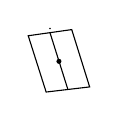
\begin{tikzpicture}[scale=0.65]
\draw (0,1.1)--(0.85,1.22)--(1.2,0.1)--(0.35,0)--cycle;
\draw (0.425,1.16)--(0.775,0.05);
\fill (0.6,0.6) circle (1.4pt);
\fill (0.425,1.24) circle (0.5pt);
\end{tikzpicture}
\end{adjustbox}
\end{center}
\SourceFigure{GELFAND-P000365}{flag-sketch-marks}{В схеме отдельная маленькая точка над верхним средним соединением и большая точка на средней линии. Над левой частью верхней линии небольшой отдельный след; верхнее правое соединение утолщено. Точное значение следа и утолщений не установлено; дополнительные узлы не восстановлены.}
Число флагов — полином по $q$, степень к-рого зав. от $n$.

\SourcePage{GELFAND-P000366}{25}
Класс смежн. опр. разбиением $n=n_1+\dots+n_k$,
$u\in U$ — элем. из этого класса.
\begin{equation*}
|P^u|=P_{n_1,\dots,n_k}(q)\text{ — полином Холла}
\end{equation*}
\underline{(число неподв. точек этого элемента).}

$u=1$ — получ. полином Пуанкаре.

Это назв. опр. полином Пуанкаре для любой расщеп. группы.

\medskip
J. A. Green, Trans. A. M. S., 1955 — рекомендуется.
\medskip

Есть оценки разм. мн-зия, леж. при этом над точкой.
\begin{equation*}
\pi:\bar R\longrightarrow R,\qquad
\dim\pi^{-1}(g)\le\frac{\dim Z_g-(n-1)}{2}.
\end{equation*}
[Неравенство в рамке.] \fbox{$Z_g$ — централизатор $g$.}

\medskip
\underline{Б. Розенфельд.}

О заметках Rego, C. R., t. 272 (1971).

[Зачёркнуто: В кас. пр-ве.]
Зад. распределение (интегрируемое) [в обводке вставлено: на $M$],
с ним связ. нек-рые когомологии.
[На правом поле, с линией к «интегрируемое»: усл. Фробениуса.]

Всякое дифф. град. кольца
[над «дифф. форм» вставлено: \Unclear{GELFAND-P000366}{forms-insert-ending}{комплексно.? / комплексна.? / комплексн.? / комплекса.?}] дифф. форм на $M$ им. вид
\begin{equation*}
d_{L_1}+i_{L_2}
\end{equation*}
($i_{L_2}$ — внутр. умнож. на вектор-форму).

\begin{gather*}
\omega(X_1,\dots,X_q)\text{ — скал. форма.}\\
L(X_1,\dots,X_p)\text{ — форма (векторнознач.).}\\
(i_L\omega)(X_1,\dots,X_{p+q-1})\text{ подст. и кососимм.}\\
d_L\omega=(d\circ i_L+(-1)^p i_L\circ d)\omega.
\end{gather*}
$L$ — форма ст. $0$ (вект. поле) — $d_L$ — произв. Ли.

[Зачёркнута формула:
\Unclear{GELFAND-P000366}{integrable-cancel}{$d_L^2=0$?}.]
Интегрируемость. (квадр. $=0$)

\SourcePage{GELFAND-P000367}{unlabelled}
Проф. \underline{Птак}.
\begin{equation*}
\dim E\ \Unclear{GELFAND-P000367}{dimension-sign}{$\le$?}\ \infty,\qquad
E\text{ с нормой}.
\end{equation*}
$q$ — показатель (крит.), если
\begin{gather*}
1^{\circ}.\quad A\in L(E),\quad
1=|A|=|A^{\Unclear{GELFAND-P000367}{a-exponent}{q?}}|
\Rightarrow |A|_\sigma=1\quad\text{(сп. радиус)}.\\
2^{\circ}.\quad \exists B,\quad 1=|B|=|B^{q-1}|,\quad
\text{но }|B|_\sigma<1.
\end{gather*}
\begin{gather*}
\ell^\infty\quad |x|=\max|x_i|,\qquad
\ell_1\quad \sum|x_i|,\qquad q(n)=n^2-n+1.\\
\ell_2\quad q(n)=n.
\end{gather*}
Сущ. $2$-мерн. пр-во, в к-ром $q=\infty$.

(По норме плохо оценивать сходимость нужны соб. знач.).

\SourceFigure{GELFAND-P000367}{danzer-diagram}{Слева замкнутый контур с уплощёнными наклонными участками; две оси со стрелками вверх и вправо, точка в пересечении, веер отрезков в верхней правой части и стрелки у левой части контура. Точное число отрезков и положение всех стрелок не восстановлены.}
$A$ — поворот на малый угол (пример Danzer'a).

$\ell_p$ — неизвестно, сущ. ли, кроме $p=2^m$.

\underline{Полезная зад. для вычислит. математики.}
\begin{equation*}
M(n)=\min\text{ по всем бан. }\le n.
\end{equation*}
$\exists$ те, по к-рым $<n$!

Сущ. послед. $M(n_k)\sim\sqrt{n_k}$.

Неизвестно, верно ли, что $\liminf M(n)=\infty$.
\begin{equation*}
\ell_4^2\underset{\ell_1}{\oplus}\ell_8^2
\end{equation*}
— [зачёркнуто:
\Unclear{GELFAND-P000367}{dimension-insert}{это?};
над зачёркнутым в обводке: здесь]
$\dim=12$, и крит. показ. $=11$.
\begin{equation*}
C(E,r,\rho)=\max\{|T^r|,\ |T|\le1,\ |T|_\sigma\le\rho\}.
\end{equation*}
[В рамке:] $0<\rho<1$.

\SourcePage{GELFAND-P000368}{26}
\underline{И. М. Гельфанд.}

С ф-ла Радона над конечн. полем. Над $F_q$ $n$-мерн. пр-во.
$(x_1,\dots,x_n)$.
[На правом поле: $q^n$ точек.]

Изв. интегр. по всем плоскостям.
\begin{equation*}
\varphi(p)=\int_{x\in p}f(x)\quad\text{(сумма)}.
\end{equation*}
$p$ — плоскость.
\begin{multline*}
\sum_{p\ni x_0}\varphi(p)
=\underbrace{\text{число точек }(n-1)\text{-мерн. проект. пр-ва}}_
{\frac{q^n-1}{q-1}}f(x_0)\\
+\frac{q^{n-1}-1}{q-1}\sum_{x\ne x_0}f(x).
\end{multline*}
[От подчёркнутого первого коэффициента линия к надписи:
столько раз счит. $x_0$.]
[После последней суммы зачёркнуто:
$+\frac{q^{n-1}-1}{q-1}$ \Unclear{GELFAND-P000368}{cancelled-term-symbol}{$A(x_0)$? / $f(x_0)$?}. Далее знак равенства.]
\begin{equation*}
\sum_x f(x)=\sum_{p\parallel p_0}\varphi(p)
[\text{зачёркнуто: }\Unclear{GELFAND-P000368}{parallel-condition}{неразборчивые знаки}]
\equiv C.
\end{equation*}
(не зав. от $p_0$) — усл. на $\varphi(p)$ — аналог теор. Пэли-Винера.
\begin{equation*}
=\frac{q^n-1}{q-1}f(x_0)+
\frac{q^{n-1}-1}{q-1}\sum_x f(x)
-\frac{q^{n-1}-1}{q-1}f(x_0).
\end{equation*}
[Сумма $\sum_x f(x)$ обведена. Под ней:
\underline{$C$ — известно.}]

\underline{Рота} — при $q\to1$ получ. перех. к прост. теоремам.

$C_k^n(q)$ — число $k$-мерных подпр. $n$-мерн. пр-ва.
\begin{equation*}
\lim_{q\to1}C_k^n(q)=C_k^n\text{ — \underline{сочетания}}.
\end{equation*}

\SourcePage{GELFAND-P000369}{unlabelled}
\underline{Кириллов.}

Рассм. произв. обобщ. ф-я $A$ на мн-зии $M$ (напр. $R^n$).

Для неё опр. фронт волны
\begin{equation*}
WF(A)\subset T^*M.
\end{equation*}
Гладк. ф-я — нулевой фронт волны (пустой).

Пусть $\xi\in T^*M$.
\begin{equation*}
\xi\notin WF(A),\quad\text{если}\quad
\langle A,\varphi e^{it\psi}\rangle=o(t^{-n}),\quad
\forall n\quad\text{при }t\to+\infty.
\end{equation*}
(при этом $d\psi=\xi$ в точке $\pi_\xi$ и $\varphi\in C_0^\infty$ любая).

Удобно изуч. ф-и, для к-рых фронт волны $\in$ лагр. мн-зия.
\begin{equation*}
N\subset M\longrightarrow\underline{\text{норм. пучок над }N}.
\end{equation*}
(перпенд. к $N$ кас. ковекторы).

Это лагр. подмн. $1/2$-й разм.

[Зачёркнуто: \Unclear{GELFAND-P000369}{pdo-cancel}{Напр.?}]
П. Д. О. — обобщ. ф-я на $M\times M$ (ядро) с фронтом
волны, таким обр. постр. из диагонали.

[Зачёркнуто: $A(p,q)=$.]
\begin{equation*}
\langle A\Unclear{GELFAND-P000369}{pairing-prefix}{i?}u\rangle
=\int e^{i\psi(x,\xi)}a(x,\xi)u(x)\,dx\,d\xi.
\end{equation*}
(Знач. $A$ на осн. ф-и $u$).

Всякое $A$ [зачёркнут знак:
\Unclear{GELFAND-P000369}{lower-cancel}{неразборчиво}]
с фр. волны, опр. так, зад. этой ф-мой.
\begin{equation*}
\text{Фр. волны }[\text{зачёркнуто: }
\Unclear{GELFAND-P000369}{wavefront-prefix}{$\varphi$?}]
\in\Lambda=\{x,\xi\mid d\psi=\xi\,dx\}.
\end{equation*}
[Под $x$: $x\in M$. Под $\xi$: $\xi\in T^*M$.]

\SourcePage{GELFAND-P000370}{27}
20/IX. А. Картан, Картье(?), Кюйпер, Делинь. — гости.
[Справа от даты: \Unclear{GELFAND-P000370}{heading-date-tail}{короткий отдельный 1-подобный штрих; значение не установлено}.]
[Под общей линией в отдельной обводке: Атья.]

\underline{И. Бернштейн.} о раб. Godbillon, Vey. Comptes rendus.

[На левом поле: $M$ — комп. мн-зие.]
На $M$ зад. форма $\omega$ (слоение $S$ коразм. $1$), к-рое интегр.
\begin{equation*}
d\omega=\omega\wedge\omega_1.
\end{equation*}
[После формулы зачёркнуто:
\Incomplete{GELFAND-P000370}{integrable-cancel}{Зачёркнутое слово не восстановлено}.]

[Зачёркнутая фраза:
\Incomplete{GELFAND-P000370}{class-cancelled-clause}{Целая зачёркнутая фраза не восстановлена}.]
Ему сопост. $\alpha_s\in H^3(M,R)$, он
[\Incomplete{GELFAND-P000370}{zero-cancel}{Зачёркнутое слово перед равенством не восстановлено}]
$=0$, если это расслоение и устойчив при деформ.,
[зачёркнуто:
\Incomplete{GELFAND-P000370}{deformation-cancel}{Зачёркнутое слово перед неравенством не восстановлено}]
$\ne0$.

Конструкция: сущ. формы $\omega_1$, $\omega_2$:
\begin{gather*}
d\omega=\omega\wedge\omega_1;\\
d\omega_1=\omega\wedge\omega_2.
\end{gather*}
Рассм. $\Omega=\omega\wedge\omega_1\wedge\omega_2$ [подчёркнуто]
— замкн. и кл. когом. не зав. от выб. $\omega_1$ и $\omega_2$.

Связь с когомологиями алгебр. есть.

[Справа:] \underline{Пример:}
$\Gamma\backslash SL(2,R)$
\Unclear{GELFAND-P000370}{quotient-end}{M?}
— комп.
$\Gamma$ — дискр. подгр.
И $\begin{pmatrix}a&0\\c&b\end{pmatrix}$ плотн. траектории —
всегда. Тогда он $\ne0$.

Слоение:
\begin{gather*}
\varphi_i:U_i\longrightarrow R,\\
\varphi_j\varphi_i:U_i\cap U_j\longrightarrow R.
\end{gather*}
[В обводке справа от формул: на отрез. прямой.]
Т. к. слои те же, то получ. $\Psi_{ij}:R\to R$ (отрезок).

Если бы $\Psi_{ij}\in$ группе, то коцикл с коэфф. в гр.
$\longrightarrow$ пучок и по нему классы когомологий. Но это псевдогруппа.

Но рассм. алгебра Ли, изом. $W_1$ — форм. вект. поля на прямой,
$f(x)\frac{d}{dx}$. Они $=0$, кроме сущ. $H^3(W_1,R)=R$.
Это и есть тот класс.

\underline{Атья.}

\underline{О спектре самосопр. эллипт. оператора.}

$X$ — комп. мн-зие,
$D$ — элл. дифф. опер., самосопр. $D^*=D$.

Дискр. спектр; соб. знач. раздел. на полож. и отр.

Пусть $D=D_t$, $t$ — парам., спектр мен. вместе с $t$.
\SourceFigure{GELFAND-P000370}{spectrum-sketch}{Вертикальная линия с поперечными штрихами разной длины, более толстый штрих в средней части. Точное число и расположение штрихов не восстановлены.}

Пусть $\underline{D_{t+1}=D_t}$ — периодичность или
\begin{equation*}
D_{t+1}=UD_tU^{-1}.
\end{equation*}
[Зачёркнутый знак расположен выше и правее $U$:
\Unclear{GELFAND-P000370}{unitary-overwrite}{на?}.]
$(U=\mathrm{const})$.
[Под второй формулой: — общее!]

\SourcePage{GELFAND-P000371}{unlabelled}
\begin{equation*}
\operatorname{Spec}D_{t+1}=\operatorname{Spec}D_t.
\end{equation*}
Спектр двигается (соб. зн. могут сдвигаться на
\Unclear{GELFAND-P000371}{shift-size}{q?}).

Можно опр. \underline{целое} число, хар. этот сдвиг.
(Поставить наблюд. в $0$ и смотреть, какая масса прошла влево и вправо.)

\SourceFigure{GELFAND-P000371}{spectrum-graphs}{Сверху графики с осями, подписями lambda и t, отметками 0 и 1, двумя вертикалями и тремя волнистыми кривыми с жирными точками на концах. Ниже между двумя почти вертикальными линиями несколько наклонных отрезков, в середине зачёркнутая надпись. Точные соединения, число нижних отрезков и зачёркнутая надпись не восстановлены.}
\Incomplete{GELFAND-P000371}{graphs-cancelled-caption}{Короткая зачёркнутая надпись в середине нижнего рисунка не восстановлена.}

\underline{Пример.} Спектр. поток $\in Z$.
\begin{equation*}
X\text{ — окр.,}\qquad D_t=-i\frac{d}{dx}+t,\qquad
Uf=e^{ix}f.
\end{equation*}
\underline{Поток} $=\pm1$ $(n\to n+1)$.

\underline{Это топ. инвариант отн. деформ. сем-ва.}

\underline{Задача:} вычислить спектр. поток через геом. данные задачи:
мн-зие, опер., $U$.

Связан с индексом.

Пусть опер. $D$ — $1$-го пор. (сист.).
Рассм. [в рамке:]
\begin{equation*}
P\equiv D_t+\frac{\partial}{\partial t}
\end{equation*}
на ф-ях $f(x,t)$, $f(x,t+1)=f(x,t)$, $x\in X$, $(U=1)$.

(если $U\ne1$, подправляем $U\otimes1$).

Это \underline{эллипт.} опер. на $X\times S^1$
(или в рассл., баз. $S^1$ слой $X$).

($D_t$ — эрм., $\frac{\partial}{\partial t}$ — косоэрм.).

\underline{Теорема.} Спектр. поток $\{D_t\}=\pm\operatorname{index}P$
[У правой скобки \Unclear{GELFAND-P000371}{theorem-parameter-limits}{верхний 1-подобный и нижний 0-подобный штрихи?; не отделены уверенно от соединённых штрихов скобки}.]
$=$ ф-ла индекса.
[У равенства и $\pm$ — большой V-образный штрих.]

Непоср. док-во сложно. Проще выраз. сп. поток ф-лой.

\underline{Эвристич. сообр.}

Пусть $D_t$ зав. от $t$ вещ.-аналит.
[Зачёркнуто:
\Incomplete{GELFAND-P000371}{analytic-cancel}{Зачёркнутое слово не восстановлено}.]
[Слева зачёркнуто:
\Unclear{GELFAND-P000371}{branch-cancel}{Начальное $t$? … конечное $t_0$? или $0$?; возможные записи $t=t_0$ / $t=0$ остаются неуверенными}.]
\begin{equation*}
\lambda_1(t),\ \lambda_1(t),\ \lambda_2(t),\dots
\end{equation*}
— аналит. ф-и!; опр. для всех $t$.
(Корни хар. полиномов; вещ. $\Rightarrow$ нет ветвлений).

\SourceFigure{GELFAND-P000371}{branch-picture}{Внизу слева почти вертикальная линия и несколько искривлённых ветвей, две группы около разных уровней. Точные пересечения и окончания ветвей не восстановлены.}

\SourcePage{GELFAND-P000372}{28}
Периодичн. $\Rightarrow$ перестановка их $\sigma$.
\begin{equation*}
-i\frac{d}{dx}+t,\qquad \sigma(n)=n+1.
\end{equation*}
Эти $\sigma$ — не произвольные.

\underline{Орбиты $\sigma$} — $4$-х классов возм.

1) конечная — соб. знач., к-рое возвращ.

2) огранич. с одной стороны (из $-\infty$ в $-\infty$ или из $+\infty$ в $+\infty$).

3) неогр. ни с одной стор.

\SourceFigure{GELFAND-P000372}{class-three-scribble}{Справа от случая 3 две ломаные или волнистые линии, несколько угловых и направленных вниз штрихов. Их точное число и соединение не восстановлены.}

\begin{equation*}
(|\lambda'(t)|< C|\lambda(t)|.)
\end{equation*}
Возрастающие и убывающие — число орбит со. классов $p$ и $q$ конечно.

Ф-и $\underline{\lambda(t)}$ на цилиндре.
3) — спирали ид. вверх или вниз.

\SourceFigure{GELFAND-P000372}{cylinder-pictures}{Слева два рисунка между вертикальными линиями: петли или спирали, сплошные и пунктирные участки, стрелка вправо на верхнем участке левого рисунка. Точные соединения и направление остальных участков не восстановлены.}

Число орбит кл. 3) — конечно. (пересеч. с \underline{горизонт.})

\underline{Спектр. поток} $\Rightarrow p-q$. (очев. отсюда).

\underline{Предположение:} пусть соб. вект. не зависят от $t$.

Тогда [зачёркнуты два слова:
\Incomplete{GELFAND-P000372}{then-cancellations}{Два зачёркнутых слова не восстановлены}.]
точн. реш.
\begin{equation*}
\left(\Unclear{GELFAND-P000372}{equation-minus}{$D_t$?}
+\frac{\partial}{\partial t}\right)u=0.
\end{equation*}
[Под плюсом вставлено «$(-)$»; к $u=0$ линия от «запиш. так:».]
\begin{gather*}
u_n=C_n\exp\left(-\int\lambda_n(t)\,dt\right),\qquad
u=\sum u_n e_n,\quad e_n\text{ — соб. вектор.}\\
\lambda_n(t+1)=\lambda_{\sigma(n)}(t).\\
\sigma(n)\longrightarrow\infty\quad\Longleftrightarrow
\text{конечн. }n\text{ и большие }t.\\
u_n(t)=C_n\exp\left(-\int_0^t\lambda_n(s)\,ds\right).
\end{gather*}
$p$ — число реш. ур-я с $+$.

$q$ — [повторные чёрточки: число реш. ур-я] с $-$,
сопр. к ур-ю с $+$.

Конечн. орбиты $\int_0^N\lambda_n(t)\,dt=0$, $N$ — период.

\underline{Индекс} $=p-q$.

В общ. случае (вектор. движ.) в ур-е $D_t+\frac{\partial}{\partial t}$
вх. доп. член, выраж. движение соб. вект.

Прежнее аналит. док-во здесь нельзя.

\SourcePage{GELFAND-P000373}{unlabelled}
\underline{Примеры.}

[Цифра $1$ обведена.]
$T:X\longrightarrow X$ — диффеом.
Опр. расслоение.
\begin{center}
\begin{adjustbox}{max width=\linewidth}
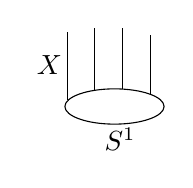
\begin{tikzpicture}[scale=0.7]
\draw (0,0) ellipse (0.9 and 0.32);
\draw (-0.86,0.12)--(-0.86,1.35);
\draw (-0.36,0.3)--(-0.36,1.42);
\draw (0.15,0.32)--(0.15,1.42);
\draw (0.66,0.23)--(0.66,1.29);
\node at (-1.18,0.75) {$X$};
\node at (0.1,-0.6) {$S^1$};
\end{tikzpicture}
\end{adjustbox}
\end{center}
Пусть функториальная ситуация $(X,g,D)$,
$g$ — рим. метрика, $D$ — самосопр. опер.

(Интересен случай неогр. с $2$-х стор. спектра).
\underline{Получается тогда: $X_t,g_t,D_t$.}

(Прим.: $d+\delta$, когда [зачёркнуто:
\Unclear{GELFAND-P000373}{example-operator-cancel}{A?};
над зачёркнутым вставлено: это] самосопр.).

Спектр. поток не зав. от выб. рим. метрики.

Если $T$ — изометрия, то $D_t=\mathrm{const}$, и сп. поток $=0$.

Инвар. — препятствие к сущ. метрики, к-рую $T$ сохраняет.

[Цифра $2$ обведена.]
$X\times S^1$, опер. $(d+\delta)_t$ на формах.
[На правом поле: скруч. с пом. этого отобр.]

Пусть дано
\begin{equation*}
\pi_1(X)\longrightarrow Z\longrightarrow S^1.
\end{equation*}
[Под второй стрелкой: характер.]
\begin{equation*}
X^{4k+1}\times S^1
\end{equation*}
— инв. Новикова с пол. $L$-полин. Хирцебруха.

\underline{Делинь в переводе Манина.} О теории мотивов.

Разные теории когомологий алг. мн-зий.

\underline{25/X-71.} \underline{С. Гельфанд.}
\underline{Шубертовские клетки.}

Horrocks, Proc. Lond. Math. Soc., 7,
\Unclear{GELFAND-P000373}{citation}{$N^{\circ}$?} $26$, 1957.

$G(N,n)$ — компл. грассм. ($n$-пл. в $C^N$).
[Под $C^N$: $E$.]
\begin{equation*}
a_1\le a_2\le\dots\le a_n\le N\text{ — набор}.
\end{equation*}
[В рамке. От набора линия к надписи на правом поле:
точки, где функц. скачки; от «скачки» линия к вставке «разм.»
над «функц.» ниже.]

Выбран фикс. флаг.
\begin{gather*}
E_1\subset E_2\subset\dots\subset E_N=E,\\
\dim E_i=i.\\
F\in\Omega(a_1,\dots,a_n),\quad
[\text{зачёркнуто: }
\Incomplete{GELFAND-P000373}{schubert-cancel}{Зачёркнутое слово не восстановлено}.]\\
\Updownarrow\\
\dim(F\cap E_{a_i+i})=i.
\end{gather*}
\begin{equation*}
\varphi(i)=\dim(F\cap E_i).
\end{equation*}
[Справа:] $\underline{a_i+i}$ — точки роста этой ф-и.

\SourcePage{GELFAND-P000374}{29}
Это клеточное разбиение грассм. \underline{мн-зия.}

\underline{Зад.} Найти все инвар. дифф. формы (кл. Черна).

Связь базиса когом. и колец.
\begin{equation*}
(*)\quad U(N)/(U(n)\times U(N-n))=G(N,n)=G/F.
\end{equation*}
Форму можно поднять на $U(N)$.

Построение форм:

$de_{ij}$.
[Справа:] $U=(e_{ij})$, $(e_{ij})$ — матр. эл. ф-я —
на $U(N)$.
\begin{equation*}
\theta_{jk}=\sum_{p=1}^N
\bar e_{k\Unclear{GELFAND-P000374}{connection-index}{p?}}\,de_{jp},
\qquad j=1,\dots,n,\quad k=n+1,\dots,N.
\end{equation*}
\begin{equation*}
\Theta_{jk}=-\frac{1}{2\pi i}\sum_{s=n+1}^N
\theta_{js}\wedge\bar\Theta_{ks},\qquad j,k=1,\dots,n.
\end{equation*}
Форма кривизны расслоения $(*)$.

Условие того, что $\omega$ — косой тенз.
[Над $\omega$ на поле: $\omega$ — форма на $G$. Справа: $G/F$.]

1) $\omega(X_1,\dots,X_k)=0$, $X_i\in T(F)$ — кас. к $F$.

2) $\omega$ — инв. отн. $F$.

Все $\Theta_{jk}$ удовл. усл. 1).

Отн. $U(N-n)$ инвар., отн. $U(n)$ преобр. сопряжением
(присоед. действие).

\medskip
\begin{equation*}
GL(n)\ni(x_{ik})_{i,k=1}^n.
\end{equation*}
Постр. полиномы от матр. элем., обл. св-вом
\begin{equation*}
p(x)=p(gxg^{-1}).
\end{equation*}
Коэфф. хар. многочлена — элем. симм. ф-и.

Надо базис лин. пр-ва.

Пусть $\lambda_1\ge\lambda_2\ge\dots\ge\lambda_n\ge0$, — целые.

$x$ — матр., $\alpha_1,\dots,\alpha_n$ — соб. числа. Надо взять
\SourcePage{GELFAND-P000375}{unlabelled}
\Unclear{GELFAND-P000375}{faint-note-complete}{симм. ф-и}
[Мелкая бледная надпись над первым определителем.]
\Unclear{GELFAND-P000375}{numerator-old-overwrite}{[Над первым элементом числителя переписан знак, похожий на $\alpha$ с индексом.]}
\begin{equation*}
\{\lambda\}=
\frac{\begin{vmatrix}
\alpha_1^{\lambda_n}&\alpha_1^{\lambda_{n-1}+1}&\cdots&\alpha_1^{\lambda_1+n-1}\\
\vdots&\vdots&&\vdots\\
\alpha_n^{\lambda_n}&\alpha_n^{\lambda_{n-1}+1}&\cdots&\alpha_n^{\lambda_1+n-1}
\end{vmatrix}}
{\begin{vmatrix}
1&\alpha_1&\cdots&\alpha_1^{n-1}\\
\vdots&\vdots&&\vdots\\
1&\alpha_n&\cdots&\alpha_n^{n-1}
\end{vmatrix}}
=\{\lambda\}(\chi_{ij})\quad\text{— полином.}
\end{equation*}
Это характер представл.
\Incomplete{GELFAND-P000375}{cancelled-dimension}{[Зачёркнут прежний фрагмент после «представл.»; видны начальное «со» и отдельные конечные штрихи, слова целиком не восстановлены.]}
[Над зачёркиванием вписано и обведено: опр. числами.]
$\lambda_1\ge\lambda_2\ge\cdots\ge$
\Unclear{GELFAND-P000375}{last-weight-sign}{$\lambda_n\ge0$}.
\begin{equation*}
\{\lambda,\text{Ⓗ}\}=\text{Ⓗ}^{\{\lambda\}}\quad\text{— обознач.}
\end{equation*}
\Unclear{GELFAND-P000375}{form-power}{$\text{Ⓗ}^{\{\lambda\}}$}
\Unclear{GELFAND-P000375}{circled-form-letter}{Ⓗ — матр. дифф. форм}
(они степ. $2$ и коммутируют).

Положим \Unclear{GELFAND-P000375}{n-after-weight}{$a_i=N'-n-\lambda_i$}.
Тогда $\int\text{Ⓗ}^{\lambda}=1$, а по другим $0$.
$\underline{\Omega(a_1,\ldots,a_n)}$.
[Справа:] \underline{степень} $=$ размерн. шуб. клетки.

\underline{Задача} (И. М. Гельфанд)
\begin{equation*}
g\in SL(2,F_q).
\end{equation*}
Групп. кольцо $\sum_g a(g)g$.
\Unclear{GELFAND-P000375}{group-ring-task}{$(a(g)\leftarrow\text{алг. замык. }F_q)$}.
Описать его.

\underline{\underline{А. Виноградов.}}

Глоб. цель — изгнать анализ из теории лин. дифф. опер.
$K$ — кольцо, (произв.). $M\longrightarrow N$, $2$ модуля над $K$.
Классич. ситуация
\begin{equation*}
K=C^{\infty}(L)\quad(L\text{ — мн-зие}),\qquad
C^{\infty}(E_1)\overset{\mathcal D}{\longrightarrow}C^{\infty}(E_2).
\end{equation*}
$K$ может быть некоммут.

\SourcePage{GELFAND-P000376}{30}
$M\overset{\mathcal D}{\longrightarrow}N$.
$k\in K$,
$k\mathcal D=$
\Incomplete{GELFAND-P000376}{cancelled-kd-equality}{[Правая часть равенства зачёркнута; прежние знаки не разобраны.]}
$k^+\mathcal D=\mathcal Dk$.
[Справа:]
\begin{align*}
(k\mathcal D)f&=k(\mathcal Df),\\
(k^+\mathcal D)f&=\mathcal D(kf).
\end{align*}
$\underline{\delta_k=k^+-k}$.

\underline{\underline{Осн. опред.}}
Дифф. опер. — аддит. отобр. $\mathcal D$: пор. $n$
\Incomplete{GELFAND-P000376}{order-overwritten}{[После видимого $n$ прежний знак густо зачёркнут; надпись целиком не читается. Под «пор.» фигурная линия.]}
\begin{equation*}
\delta_{k_0}\delta_{k_1}\cdots\delta_{k_n}\mathcal D=0,
\qquad\underline{\underline{\forall k_0,\ldots,k_n}}.
\end{equation*}
В классич. случае совпад. с обычным.
Так алгебр. стр. теор. гомол. де Рама и т. д.
\Unclear{GELFAND-P000376}{spencer-note}{(Спенсер. и пр.)}

$Diff_n^+(M,N)$ — все эти операторы.
модуль с умн. $\underline{\underline{k^+}}$.
\begin{align*}
Diff_n^+(M,N)&\overset{def}{=}Hom_K(M,Diff_n^+N),\\
Diff_n(M,N)&\overset{def}{=}Hom(J^n(M),N).
\end{align*}
\SourceFigure{GELFAND-P000376}{hom-definition-diagram}{Две колонки определений: слева $Diff_n^+(M,N)$ над $Hom_K(M,Diff_n^+N)$, между ними две вертикальные черты и «def», от «def» короткая стрелка вправо вниз к $Diff_n^+N$; справа $Diff_n(M,N)$ над $Hom(J^n(M),N)$, «def» при двух чертах и стрелка вертикально вниз.}
\begin{equation*}
Diff_n^+(N)=Diff_n^+(K,N)\Longrightarrow Diff_n^+(N).
\end{equation*}
[Под правым выражением:] \underline{коджеты}.
$\Longrightarrow$ теор. сущ. см.
$J^n(K)$
\Incomplete{GELFAND-P000376}{cancelled-after-jets}{[После $J^n(K)$ зачёркнут мелкий знак, целиком не разобран.]}
— теор. сущ. тоже есть.
В $Diff_nK$ рассм. алг. опер. порожд. $k,k^+$.
\begin{equation*}
J^n(K)=\{k,k_N^+\}.
\end{equation*}
\Unclear{GELFAND-P000376}{jet-generators}{$\{k,k_N^+\}$}

\SourcePage{GELFAND-P000377}{unlabelled}
$D_i$ —
\Incomplete{GELFAND-P000377}{cancelled-functor-word}{[Слово перед «функторы» зачёркнуто несколькими горизонтальными линиями, целиком не восстановлено.]}
функторы $D_i(M)$ (гомологии де Рама).
Определим по индукции.
$D=D_1$ — дифференцирования $K$ в $N$ — обознач. $D(N)$.
$K\overset{\nabla}{\longrightarrow}N$ дифференцир., если
\begin{equation*}
\nabla(k_1,k_2)=k_1\nabla k_2+k_2\nabla k_1.
\end{equation*}
Это д. оп. $1$-го пор.
[Справа дописано:] $(-k_1k_2\nabla(1))$.
Это $D(N)$ (вект. поля со зн. в $N$).
$D$ — обычн. вект. поля.
\begin{equation*}
D_2(N)=D\{D(N)\subset Diff_1^+N\}.
\end{equation*}
$D\hookrightarrow Diff_1^{(+)}$.
[Справа в скобке:] $D$ —
\Unclear{GELFAND-P000377}{module-cancelled}{[Зачёркнуто: правый]}
\underline{левый} модуль,
$Diff_1^+$ — правый; $D$ — подмн-во, а не подмодуль.
В $Diff_1^{(+)}$ не подмодуль — влож. — дифф. опер. $1$-го пор.
$D_2(N)$ — дифф. $K$ в $Diff_1^+N$, к-рые уход. в $D(N)$.
\begin{equation*}
D_i(N)=D\{D_{i-1}(N)\subset(Diff_1^+)^{i-1}(N)\}.
\end{equation*}
(по индукции).

\underline{1/XI-71}
[Над и под XI горизонтальные черты, после года правая скобка.]
\underline{Ур-е Гамильт.-Якоби:}
\begin{equation*}
\delta_{k_1}\cdots\delta_{k_1}\mathcal D
\quad\text{— лев. часть ур-я Гам.-Якоби.}
\end{equation*}
\Unclear{GELFAND-P000377}{hamilton-repeated-index}{$\delta_{k_1}\cdots\delta_{k_1}\mathcal D$}
(посчитать) ($k_1$ — всюду одно и то же).

\underline{Теор. сущ. для}
\Unclear{GELFAND-P000377}{jets-theorem-index}{$\underline{J^n(M)}$}:
\begin{equation*}
K\otimes_{\mathbb Z}M/\Pi_s=J^s(M).
\end{equation*}
$\Pi_s$ — подмодуль в $K\otimes_{\mathbb Z}M$, порожд. необх. соотн.
\begin{align*}
k(k'\otimes m)&=kk'\otimes m,\\
\bar k(k'\otimes m)&=k'\otimes km.
\end{align*}

\SourcePage{GELFAND-P000378}{31}
\begin{equation*}
\Delta_{k_0\ldots k_s}=(\bar k_0-k_0)\cdots(\bar k_s-k_s).
\end{equation*}
Рассм. подмодуль, порожд. этими $\Delta$.
\begin{equation*}
K\otimes_{\mathbb Z}M=\underline A\supset\Delta(A)=\underline{\Pi_s}
\quad\text{(обычное опред. джетов).}
\end{equation*}
\Incomplete{GELFAND-P000378}{cancelled-upper-line}{[Зачёркнута вся строка: «В простейш. случае просто»; формульные штрихи отмечены отдельно, последние наложенные штрихи не восстановлены.]}
\Unclear{GELFAND-P000378}{cancelled-upper-target}{$Diff_s^{(+)}(K,N)$ [зачёркнуто; целевой знак $N/M$]}
[На правом поле:] \underline{$J^s(K)$ проще, чем в общем случае.}
$D_1(M)$ — дифф. опер. без своб. члена.
$D_1(M)=D(M)$ (дифф. $K$ со знач. в $M$).
$D(M)\subset Diff_1M$.
\begin{equation*}
A\in D_1(M)\overset{def}{\Longleftrightarrow}
A(k_1,k_2)
=A(k_1)k_2+k_1A(k_2).
\end{equation*}
\Unclear{GELFAND-P000378}{derivation-argument}{$A(k_1,k_2)$}
[На правом поле за вертикальной линией:]
$D_k(M)$ — левый модуль. (отн. умн. $k$).
$D_0(M)=M$.
\begin{align*}
D_2(M)&=D_1(D_1(M)\subset Diff_1^+(M)),\\
D_{k+1}(M)&=D_1(D_k(M)\subset Diff^+_{\underbrace{1\,1\ldots1}_{k\text{ раз}}}(M)).
\end{align*}
[Справа:] $k$-кратное применение функтора $Diff_1^+(M)$.
\begin{equation*}
D_1(D_1(M)\subset Diff^+(M)).
\end{equation*}
\Incomplete{GELFAND-P000378}{cancelled-nonmodule}{[Зачёркнута надпись над «не подмодуль»; видны части «не» и «подмод…», целиком не восстановлена.]}
не подмодуль в структ. $Diff^+(M)$.
[В рамке справа:] Дифф.
\Incomplete{GELFAND-P000378}{boxed-cancelled-word}{[После «Дифф.» перед $K$ зачёркнуто слово, целиком не читается.]}
$K$ в $Diff_1^+(M)$,
\Incomplete{GELFAND-P000378}{boxed-prefix-complete}{[Перед «у» зачёркнут короткий фрагмент, целиком не разобран.]}
у к-рого знач. лежат в подмн-ве $D_1(M)$.

\begin{adjustbox}{max width=\linewidth}
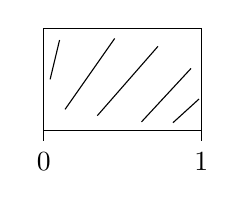
\begin{tikzpicture}[x=1cm,y=1cm]
\draw (0,0) rectangle (2,1.3);
\draw (0.08,0.65)--(0.2,1.15);
\draw (0.27,0.27)--(0.9,1.17);
\draw (0.68,0.19)--(1.45,1.07);
\draw (1.24,0.11)--(1.87,0.79);
\draw (1.64,0.1)--(1.97,0.4);
\draw (0,-0.13)--(0,0.18);
\draw (2,-0.13)--(2,0.18);
\node[below] at (0,-0.15) {$0$};
\node[below] at (2,-0.15) {$1$};
\end{tikzpicture}
\end{adjustbox}
$0=1$ со склеенными концами.
[Справа:] $M$ — функции. $\underline{\underline{M=K}}$.
\begin{equation*}
D_1(M)=\left\{a\right.
\end{equation*}
\Incomplete{GELFAND-P000378}{overwritten-a-argument}{[Аргумент после $a$ густо переписан и зачёркнут, целиком не разобран.]}
$\dfrac{\partial}{\partial x}+b\dfrac{\partial}{\partial y}$.
[У выражения видна только открывающая фигурная скобка.]
$Diff_1^+:a\dfrac{\partial}{\partial x}+b\dfrac{\partial}{\partial y}+c$.
$K(x)\longrightarrow$
\Incomplete{GELFAND-P000378}{last-field-cutoff}{[Сразу после стрелки зачёркнут короткий префикс, целиком не читается.]}
\Unclear{GELFAND-P000378}{last-field-coefficients}{$a_k\dfrac{\partial}{\partial x}+b_k\dfrac{\partial}{\partial y}$}.
[Строка у нижней границы кадра.]

\SourcePage{GELFAND-P000379}{unlabelled}
\begin{align*}
a(k_1k_2)\frac{\partial}{\partial x}+b(k_1k_2)\frac{\partial}{\partial y}
&=a(k_2)\frac{\partial}{\partial x}k_1+b(k_2)\frac{\partial}{\partial x}k_1+\\
&\quad+a(k_1)\frac{\partial}{\partial x}k_2+b(k_1)\frac{\partial}{\partial x}k_2;
\end{align*}
\Unclear{GELFAND-P000379}{repeated-x-denominators}{[В четырёх слагаемых справа в знаменателях написано $\partial x$, в том числе при $b$.]}
Отсюда
$a(k_1k_2)=a(k_2)k_1+a(k_1)k_2$
и $b$ — дифф. и ещё условие:
\begin{equation*}
a(k_2)\frac{\partial k_1}{\partial x}+a(k_1)\frac{\partial k_2}{\partial x}
+b(k_2)\frac{\partial k_1}{\partial x}+b(k_1)\frac{\partial k_2}{\partial x}
\end{equation*}
\Unclear{GELFAND-P000379}{condition-cancelled-tail}{[После суммы зачёркнуто $=0$, затем многоточие и $=0$.]}
\begin{equation*}
\left(a(k_2)\frac{\partial}{\partial x}+b(k_2)\frac{\partial}{\partial y}\right)k_1+\sim=0.
\end{equation*}
\begin{equation*}
D_1(k_2)k_1+D_1(k_1)k_2=0,
\qquad k\longrightarrow D_1(k).
\end{equation*}
\Unclear{GELFAND-P000379}{condition-d-one-index}{$D_1(k_2)k_1+D_1(k_1)k_2=0$}
\fbox{$D_1(k_2)k_1+D_1(k_1)k_2=0$} — требование.
[Горизонтальная разделительная линия.]
\Incomplete{GELFAND-P000379}{cancelled-first-mark}{[На левом поле перед $D_k(M)$ зачёркнут отдельный знак, целиком не разобран.]}
$\underline{\underline{D_k(M)}}$ — $k$-формы на
\Incomplete{GELFAND-P000379}{cancelled-manifold-symbol}{[Между «на» и «мн-зии» густо зачёркнут знак; целиком не восстановлен.]}
мн-зии со знач. в $M$.
\Unclear{GELFAND-P000379}{cancelled-definition-word}{[Под строкой слева зачёркнуто: Опр-е.? / Опр-о.? / Опр.?]}
\Incomplete{GELFAND-P000379}{cancelled-after-k-forms}{[Под словом «формы» зачёркнута отдельная надпись, целиком не восстановлена.]}
\begin{equation*}
Diff^+_{\underbrace{1,1,\ldots,1}_{k\text{ раз}}}
=(Diff_1^+)^k=Diff_1^+(\underbrace{\cdots Diff_1^+\cdots}_{k\text{ раз}}).
\end{equation*}
\begin{equation*}
(Diff_1^+)^2(M)=Diff_1(K,Diff_1^+M).
\end{equation*}
\underline{Определение внешних дифф. форм.}
(комплекс де Рама над кольцом $K$)
\begin{equation*}
D_i(M)\overset{def}{=}Hom_K(\Lambda_i,M).
\end{equation*}
[От «def» изогнутая стрелка к $\Lambda_i$.]
\begin{equation*}
\underline{\underline{\Lambda_i=\Lambda_i(K)}}.
\end{equation*}
\Unclear{GELFAND-P000379}{lambda-argument-correction}{[В аргументе перед $K$ зачёркнуто: $M$.]}
\underline{Теорема:} существуют предст. объекты.
$K=\mathbb Z_2$ будет $D_2\ne0$! ($2$-мерн. класс. де Рама).

\SourcePage{GELFAND-P000380}{32}
Рассм. групп. кольцо
\Unclear{GELFAND-P000380}{gamma-two-ring}{$\Gamma_2(\mathbb Z_2)$}
(с коэфф. из $\mathbb Z_2$).
Все гр. когом. де Рама — $\mathbb Z_2$.
Для \underline{групп. колец} когом. \underline{де Рама} — \underline{когом.} групп!
\begin{equation*}
0\longrightarrow J\longrightarrow K\otimes K\overset{\text{произв.}}{\longrightarrow}K\longrightarrow0.
\end{equation*}
[Слева над $0\to J$: $\Lambda_1^{\text{стар}}(K)$, стрелка к $J$.]
\begin{equation*}
J^1/J^2=\Lambda_1,
\quad\text{ост. — внешние степени.}
\end{equation*}
\Unclear{GELFAND-P000380}{augmentation-powers}{$J^1/J^2=\Lambda_1$}
От поля эти когом. будут $0$, а Виноградовские $\ne0$.
Это опр. неестеств. в категорном смысле.
Они не опр. для \underline{некоммут.} колец.
Это единств. естеств. опред. в категории колец.

\underline{Дифференциал $d$.}
\begin{equation*}
D_k\longrightarrow D_{k-1}(Diff_1^+)
\quad\text{— \underline{морфизм функторов}.}
\end{equation*}
(в других терминах $d$).
т. е. $D_k(M)\longrightarrow D_{k-1}(Diff_1^+(M))$. естеств. отобр.
\Incomplete{GELFAND-P000380}{tiny-cancelled-mark}{[Под отображением зачёркнут мелкий отдельный знак; целиком не восстановлен.]}
\begin{equation*}
D_1=D\longrightarrow Diff_1^+
(=D_0(Diff_1^+)).
\end{equation*}
\Unclear{GELFAND-P000380}{d-subscript-overwrite}{$D_1$}
[Под стрелкой:] влож.
$D_1\longrightarrow D_0(Diff_1^+)$.
(не влож. мод., а дифф. опер. $1$-го порядка).
[Справа:] $Diff_n\longrightarrow Diff_n^+$ (дифф. опер. порядка $n$).

Индукция:
\begin{align*}
D_k&=D_1\{D_{k-1}\subset(Diff_1^+)^{k-1}\},\\
D_{k-1}(Diff_1^+)&=D_1\{D_{k-2}(Diff_1^+)\subset(Diff_1^+)^{k-2}(Diff_1^+)\}.
\end{align*}
[Под правой частью, две вертикальные черты:]
$(Diff_1)^{k-1}$.
Предполож. индукт., что $D_{k-1}\subset D_{k-2}(Diff_1^+)$,
и тогда получим:

\SourcePage{GELFAND-P000381}{unlabelled}
$D_k\subset D_{k-1}(Diff_1^+)$.
Это
\Incomplete{GELFAND-P000381}{cancelled-before-injective}{[Перед «инъективный» зачёркнут короткий знак или фрагмент, целиком не разобран.]}
инъективный морфизм функторов, то есть
$\forall$ модуля $M$: $D_k(M)\subset D_{k-1}(Diff_1^+(M))$,
[Под включением:] подмодуль.
Реализуем на языке дифф. форм:
\begin{adjustbox}{max width=\linewidth}
\begin{tikzcd}
\Lambda_{i-1}\arrow[r,"\nabla"]&\Lambda_i\arrow[d,"h"]\\
&M
\end{tikzcd}
\end{adjustbox}
\Unclear{GELFAND-P000381}{lambda-indices}{[Индекс $i-1$ у левого $\Lambda$ и $i$ у правого написаны поверх усиленных штрихов.]}
[В рамке слева:] $\nabla\in Diff_1^+(\Lambda_{i-1},\Lambda_i)$.
[Справа:]
$D_i(M)=Hom(\Lambda_i,M)$.
$\Lambda_i=\Lambda_i(K)$ — универс. объект. (модуль над $K$).
[От $\Lambda_i$ стрелка к подписи:] \underline{обычные дифф. формы}.
[Над «обычные»:] \Unclear{GELFAND-P000381}{ordinary-emphasis-mark}{[Отдельный толстый вертикальный штрих, похожий на верхнюю часть восклицательного знака; отдельная точка не установлена.]}
\begin{equation*}
D_i(M)\overset{\alpha_i}{\longleftrightarrow}D_{i-1}(Diff_1^+(M)).
\end{equation*}
$h\in Hom(\Lambda_i,M)\overset{\alpha_i}{\longleftrightarrow}$
\Incomplete{GELFAND-P000381}{cancelled-hom-prefix}{[Перед $Hom$ густо зачёркнут короткий фрагмент; целиком не восстановлен.]}
$Hom(\Lambda_{i-1},Diff_1^+(M))$.
Пусть зад. дифф. опер. $1$-го пор. $\Lambda_{i-1}\overset{\nabla}{\longrightarrow}\Lambda_i$.
Тогда каждому $h:\Lambda_i\longrightarrow M$ сопост. композиция
$h\circ\nabla\in Diff_1^+(\Lambda_{i-1},M)$.
\begin{equation*}
\forall\nabla\Longrightarrow D_i\overset{\alpha_i(\nabla)}{\longrightarrow}D_{i-1}(Diff_1^+).
\end{equation*}
[Под стрелкой:] будет постр.
\begin{align*}
h&\longrightarrow h\circ\nabla\in Diff_1^+(\Lambda_{i-1},M)\Longrightarrow\\
&\Longrightarrow Hom(\Lambda_{i-1},Diff_1^+M)=Hom(J^1\Lambda_{i-1},M).
\end{align*}
[Между первой строкой и следующим $Hom$ две вертикальные черты; равенство к последнему $Hom$ тоже двумя вертикальными чертами.]
И сопр. на $M$
\Incomplete{GELFAND-P000381}{cancelled-arrow-expression}{[Зачёркнутая надпись, затем усиленная стрелка вправо, затем зачёркнуто «дифф.»; первая надпись целиком не восстановлена.]}
гомом. $J^1\Lambda_{i-1}\longrightarrow\Lambda_i$,
т. е. дифф. опер. $\Lambda_{i-1}\longrightarrow\Lambda_i$.
Взять $M=\Lambda_i$ и тожд. отобр. даёт то, что надо.

\SourcePage{GELFAND-P000382}{33}
$Hom(\Lambda_i,M)\overset{\alpha_i}{\longleftrightarrow}Hom(\Lambda_{i-1},Diff_1^+(M))$.
$M=\Lambda_i$ и слева $id$.
Элем. $Hom(\Lambda_{i-1},Diff_1^+(M))$ по опр. есть дифф. оператор
$1$-го пор. из $\Lambda_{i-1}$ в $M$.
(Находим $\nabla$, к-рый сущ. и единственно).
Надо док., что $\underline{d^2=0}$.
[Под формулой горизонтальная черта с вертикальными концами.]
Рассмотрим
\begin{adjustbox}{max width=\linewidth}
\begin{tikzcd}
D_{i+1}\arrow[r]\arrow[rrd]&D_i(Diff_1^+)\arrow[r]&D_{i-1}(Diff^+_{1,1})\arrow[d]\\
&&D_{i-1}(Diff_2^+)
\end{tikzcd}
\end{adjustbox}
\underline{В сторону:}
Кольцо $F_2(\mathbb Z_2)$ — не совпад. с классическими.
$0,1,x$,
\Incomplete{GELFAND-P000382}{cancelled-group-ring-entry}{[После $x$ в перечислении зачёркнут отдельный элемент, целиком не восстановлен.]}
$1+x$, $(x^2=1)$.
$y=x+1$, тогда $\underline{\underline{y^2=0}}$.
$0,1,y,1+y$, где $\underline{y^2=0}$.
[Горизонтальная разделительная линия.]
Будет построен опер. Спенсера (граничный).
[Над схемой справа:] $Diff_1(Diff_k)$.
\SourceFigure{GELFAND-P000382}{spencer-complete-diagram}{Слева сверху $D_{i+1}(Diff_k^+)$, справа сверху $D_i(Diff^+_{1,k})$, ниже справа $D_i(Diff^+_{k+1})$. Стрелка слева направо, над ней $\alpha_{i+1}(Diff_k^+)$; от верхнего правого выражения стрелка вниз к нижнему; из левого выражения диагональная стрелка вправо вниз, надпись $Spc$ на ней перечёркнута; последний знак похож на $c/e$. Снизу слева изогнутая стрелка подходит к началу верхней горизонтальной, подпись «дифф. опер. 1-го пор.». Под диагональной вертикальная скобка к подписи «Это гом. Спенсера»; «Спенсера» подчёркнуто. После $k$ в обоих верхних выражениях зачёркнуты индексные фрагменты, отмеченные отдельно.}
\Unclear{GELFAND-P000382}{spencer-label-endings}{[Четыре подписи: $Spc/Spe$ (возможен нижний $e$-подобный знак); диагональная перечёркнута, три нижние текущие.]}
\Unclear{GELFAND-P000382}{spencer-left-degree}{$D_{i+1}$ [вертикальные части знака после $i$ прерывисты]}
\Unclear{GELFAND-P000382}{spencer-start-cancelled-index}{[После $k$ слева зачёркнута связка и цифра, похожая на $2$.]}
\Incomplete{GELFAND-P000382}{spencer-end-cancelled-index}{[После $k$ справа зачёркнут дополнительный индексный фрагмент, целиком не восстановлен.]}
[Справа:] — гом. модулей (композ. дифф. опер. даёт отобр.
$Diff^+_{1,k}\longrightarrow Diff_{k+1}$).
\underline{Комплекс Спенсера:}
\begin{equation*}
M\overset{\Delta}{\longleftarrow}Diff_k^+M
\overset{Spc}{\longleftarrow}D(Diff_{k-1}^+M)
\overset{Spc}{\longleftarrow}\cdots\overset{Spc}{\longleftarrow}
D_i\quad\text{[зачёркнуто]}
\end{equation*}
\Unclear{GELFAND-P000382}{spencer-cancelled-endpoint}{$D_i$ [зачёркнуто]}

\SourcePage{GELFAND-P000383}{unlabelled}
$\longleftarrow D_i(Diff^+_{k-i}M)\longleftarrow\cdots$
Это резольв. Спенсера
\Unclear{GELFAND-P000383}{resolvent-parenthesis}{(корезольв. См.)}
[Над следующей строкой мелко:] \Unclear{GELFAND-P000383}{small-jets-note}{там} для $J$.
\begin{equation*}
M\longleftarrow Diff_{\infty}^+\{M\}
\longleftarrow D_1(Diff_{\infty}^+\{M\})
\longleftarrow\cdots\longleftarrow D_i(Diff_{\infty}^+M)\longleftarrow\cdots
\end{equation*}
\begin{equation*}
Diff_{\infty}^+M=\underset{\longrightarrow}{\lim}Diff_i^+
\quad(Diff_i^+\subset Diff_{i+1}^+).
\end{equation*}
\underline{Это} \underline{комплекс}.
И отобр. (пока не опред.)
$Diff_k^+M\longrightarrow M$.
\begin{equation*}
Diff_s^+(M,N)\overset{def}{=}Hom_K(M,Diff_s^+N).
\end{equation*}
Пусть $Diff^+N\overset{\Delta}{\longrightarrow}N$;
$\Delta$ — опер. порядка $s$.
Тогда по гом. $h:M\longrightarrow Diff^+N$ стр. композиция.
(надо взять в кач. $M$ $Diff_s^+N$ и тожд. отобр.
$id\in Hom(M,Diff_s^+N)$; получ. $Diff_s^+N\longrightarrow N$).
Это опред. $1$-го морфизма.
$\underline{\underline{\Delta\in Diff_s^+(K,M)\longrightarrow\Delta(1)}}$.

\underline{Заголовки:}
Все резольв. Спенсера не в коорд. форме (отличие от Спенсера).
Индекс над любым кольцом.
Гамильтонов формализм для $\forall$ кольца.
\underline{\underline{След. раз — продолжение.}}

\SourcePage{GELFAND-P000384}{34}
8/XI [XI ограничено сверху и снизу чертами.]
[Пустые скобки на левом поле.]
\underline{Лемма 1.}
$Diff_n^+(M,N)$ при фиксир. $N$ — функтор от $M$ (контравар.).
\begin{adjustbox}{max width=\linewidth}
\begin{tikzpicture}
\node[draw,ellipse] (a) at (0,0) {мод.};
\node[draw,ellipse] (b) at (2,0) {мод.};
\draw[->] (a)--(b);
\end{tikzpicture}
\end{adjustbox}
(а если брать $Diff_n(M,N)$, то это функтор от $N$ при фикс. $M$ (ковар.)).
\underline{Док-во:}
$\mathcal F^+_{N,n}(M)=Diff_n^+(M,N)$.
Если $f:M_1\longrightarrow M_2$ гом. мод. $\Longrightarrow$
\begin{equation*}
\mathcal F^+_{N,n}(f):Diff_n^+(M_2,N)\longrightarrow Diff_n^+(M_1,N).
\end{equation*}
[Справа в рамке:]
\Unclear{GELFAND-P000384}{variance-proof-inset}{$D:M_2\longrightarrow N\leadsto D\circ f:M_1\longrightarrow M_2$}.
И это есть гомоморфизм модулей, т. к.
\Incomplete{GELFAND-P000384}{derivative-cancel-complete}{[Перед $D(kf)$ зачёркнут отдельный фрагмент, целиком не восстановлен.]}
\begin{equation*}
D(kf)=(Dk)f=\underbrace{(k^+D)f}=Dfk=k^+(Df)\Longrightarrow(k^+D)f=k^+(Df).
\end{equation*}
[Под $(k^+D)f$ короткая фигурная линия.]
Аналогично, если рассм. $Diff_n(M,N)$ как функтор от $N$,
то $f$ надо послать слева и это тоже получ. гомом. модулей.

[Пустые скобки на левом поле.] \underline{Лемма 2.}
Пусть $A\in Diff_1(K,M)$. Тогда
\begin{equation*}
A(k_1k_2)=k_1A(k_2)+k_2A(k_1)-k_1k_2A(1).\qquad(1)
\end{equation*}
и наоборот, если $A:K\longrightarrow M$ — аддит. отобр., удовл. (1),
то $A\in Diff_1(K,M)$.
\underline{Док-во:} Общая ситуация $A\in Diff_1(N,M)\Longleftrightarrow$
\begin{equation*}
Ak_0k_1=k_0Ak_1+k_1Ak_0-k_0k_1A\quad(\forall k_0,k_1).\qquad(2)
\end{equation*}
Для $N=K$ это значит, что
\begin{equation*}
A(k_0k_1k)=k_0A(k_1k)+k_1A(k_0k)-k_0k_1A(k).\qquad(3)
\end{equation*}
Полагая $k=1$, получим (1). Обратно пусть (1)
\Unclear{GELFAND-P000384}{tiny-proof-word}{вып.}
[Мелкая вставка над следующей строкой:] $(\forall k_0,k_1,k)$.
Док-м
\Unclear{GELFAND-P000384}{proof-reference-three}{(3)}.
\begin{align*}
A(k_0k_1k)&=A(k_0(k_1k))=k_0A(k_1k)+k_1(kA(k_0))-k_0k_1kA(1)=\\
\bigl(kA(k_0)&=A(kk_0)+kk_0A(1)-k_0A(k)\bigr)\\
&=k_0A(k_1k)+k_1A(k_0k)+
k_1kk_0A(1)\ \text{[зачёркнуто]}
-k_1k_0A(k)-k_0k_1kA(1)\ \text{[зачёркнуто]}.\\
&=k_0Ak_1k+k_1Ak_0k-k_0k_1Ak,
\end{align*}
что и требовалось.
\Unclear{GELFAND-P000384}{middle-cancel-complete}{$k_1kk_0A(1)$ [зачёркнуто]}
[Под средними слагаемыми предпоследней строки фигурная линия.]
\underline{Следствие:} $A\in Diff_1(K,M)\Longrightarrow A-A(1)$ — дифференцирование $K$ в $M$.

\underline{Лемма 3.} Пусть
\Unclear{GELFAND-P000384}{lemma-three-first-index}{$A_1$}
$\in Diff_m(M_1,M_2)$, $B\in Diff_n(M_2,M_3)$.
Тогда $B\circ A\in Diff_{m+n}(M_1,M_3)$.
\underline{Док-во:} индукция по $\underline{m+n}$.
При $m+n=0$ ($m=n=0$) всё очевидно.
Пусть для $m+n\le d-1$ док. Пусть $m+n=d$.
\begin{equation*}
\delta_k(B\circ A)=kBA-BAk=(kB-Bk)A+B(kA-Ak)
=(\delta_kB)A+B(\delta_kA)\quad\blacksquare
\end{equation*}
\SourcePage{GELFAND-P000385}{unlabelled}

\underline{Лемма 4.} Сущ. канонич. дифф. оператор пор. $n$:
\begin{gather*}
\operatorname{Diff}_n^+(K,N)\longrightarrow N,\\
C:\quad A\longmapsto A(1).
\end{gather*}
\underline{Док-во.}
\begin{multline*}
(\delta_k C)(A)=(kC-Ck)(A)=kA(1)-CAk\\
=kA(1)-Ak(1)=(\delta_k A)(1).
\end{multline*}
отсюда
\begin{equation*}
(\delta_{k_0}\delta_{k_1}\dots\delta_{k_n}C)(A)
=(\delta_{k_0}\delta_{k_1}\dots\delta_{k_n}A)(1)=0
\end{equation*}
и $C$ — дифф. опер.

\underline{Следствие:} сущ. канонич. гомоморфизм
\begin{equation*}
\operatorname{Hom}_K(M,\operatorname{Diff}_n^+(K,N))
\longrightarrow\operatorname{Diff}_n^+(M,N),\qquad
f\longmapsto C\circ f.
\end{equation*}
[Перед $C\circ f$ зачёркнута формула.]
\Incomplete{GELFAND-P000385}{consequence-cancel}{Зачёркнутая формула перед заменой $C\circ f$ не восстановлена.}

(Пров. того, что это гом. модулей:
$kf\longmapsto C\circ kf=C\circ fk=k^+(C\circ f)$, и и т. д.)

\underline{Лемма 5.}

Сущ. кан. гомоморфизм:
\begin{gather*}
\operatorname{Diff}_n^+(M,N)\longrightarrow
\operatorname{Hom}_K(M,\operatorname{Diff}_n^+(K,N)),\\
A\longrightarrow\{m\longmapsto A(km)\}.
\end{gather*}
\underline{Док-во.}

1) Проверка того, что $A(km)$ ($m$ — фикс.) $\in\operatorname{Diff}_n^+(K,N)$ —
— это дифф. опер. на подмодуле (огранич. большого д. опер.) $=$
\begin{gather*}
K\longrightarrow M\longrightarrow N,\\
k\longrightarrow km\overset{A}{\longrightarrow}A(km).
\end{gather*}
[На правом поле:] канон. гомоморф. и дифф. опер. пор. $n$.

2) Пров. того, что $g:m\longmapsto A(km)$ есть
$\operatorname{Hom}_K(M,\operatorname{Diff}_n^+(K,N))$.

[Перед формулой зачёркнуто
$\Unclear{GELFAND-P000385}{g-old}{g\dots}$.]
\begin{equation*}
\Unclear{GELFAND-P000385}{g-add-bracket}{g(m_1+m_2)(k)}
=A(km_1+km_2)=A(km_1)+A(km_2)=g(m_1)(k)+g(m_2)(k).
\end{equation*}
\begin{multline*}
g(k_0m)(k)=A(kk_0m)=A(k_0km)=(Ak_0)(km)\\
=(k_0^+A)(km)=k_0^+g(m).
\end{multline*}

3) Пров. того, что $A\longrightarrow\{m\longmapsto A(km)\}$ есть гомоморфизм.
\begin{equation*}
k^+A\longrightarrow\{m\longrightarrow k^+A(km)\}
=k\{m\longrightarrow A(km)\},\quad\text{и и т. д.}
\end{equation*}

\underline{Лемма 6.}

Построенные отображения (следствие леммы 4 и лемма 5) вз. обратны и
задают изом. модулей
\begin{equation*}
\operatorname{Diff}_n^+(M,N)\cong
\operatorname{Hom}_K(M,\operatorname{Diff}_n^+(K,N)).
\end{equation*}
\underline{Док-во.}
\Incomplete{GELFAND-P000385}{proof-six-cancel}{Зачёркнутое слово перед «Пусть» не восстановлено.}
Пусть $A\in\operatorname{Diff}_n^+(M,N)$, строим
$A'\in\operatorname{Hom}_K(M,\operatorname{Diff}_n^+(K,N))$:
\begin{equation*}
(A'm)(k)=A(km).
\end{equation*}
Теперь по $A'$ строим $A''\in\operatorname{Diff}_n^+(M,N)$ по формуле
\begin{equation*}
A''_m=C\circ A'm=(A'm)(1)=A(m),\quad\text{т. е. }A''=A.
\end{equation*}
Пусть, обратно, $A'\in\operatorname{Hom}_K(M,\operatorname{Diff}_n^+(K,N))$.
Строим $A''\in\operatorname{Diff}_n^+(M,N)$

\SourcePage{GELFAND-P000386}{35}

формулой $A''m=(A'm)(1)$ и затем
$A'''\in\operatorname{Hom}_K(M,\operatorname{Diff}_n^+(K,N))$
как
\begin{multline*}
(A'''m)(k)=A''(km)=(A'(km))(1)=k^+A'(m)(1)=(A'(m)k)(1)\\
=A'(m)(k),\quad\text{т. е. }A'''=A'.
\end{multline*}
\Incomplete{GELFAND-P000386}{proof-end-cancel}{Короткое зачёркнутое слово перед чёрным квадратом не восстановлено.}
$\blacksquare$

Итак, доказано, что \fbox{$\operatorname{Diff}_n^+N=\operatorname{Diff}_n^+(K,N)$.}

\SourcePage{GELFAND-P000387}{unlabelled}

15/XI. \underline{И. М. Гельфанд.}

$G$ — группа Ли, $X$ — пр-во, $G$ — действует на $X$ транзитивно
($X$ — однородное пр-во).

Главное однор. пр-во: $G$ действ. на $X$ без неподв. точек
($xg=y\Rightarrow g$ — единственно).

\underline{То же в терминах алгебры Ли:}

Пусть на $X$ действ. алгебра Ли $\mathfrak{g}$.
\begin{gather*}
\xi\in\mathfrak{g}\leadsto\text{векторное поле на }X;\quad a(\xi),\\
\xi_1+\xi_2\leadsto a(\xi_1)+a(\xi_2);\\
[\xi_1,\xi_2]\longrightarrow[a(\xi_1),a(\xi_2)].
\end{gather*}
\underline{Однородное пр-во:} если $\mathfrak{g}\longrightarrow TX_x$ эпим. $\forall x$
($a(\xi)_x$ порождают всё $X$).

(Можно док., что иногда это означает обычную однородность)

очень редко.

Когда можно \Unclear{GELFAND-P000387}{group-abbreviation}{дог.} до группы.

\underline{когда $\mathfrak{g}$ конечномерна.}

Главное однор. пр-во: отобр. $\mathfrak{g}\longrightarrow TX_x$
\underline{изоморфизм.}

\underline{Обычный случай:}

фиксир. $x_0$, получается $x_0g=y$. $g\leftrightarrow y$, $X\cong G$
и преобр. правый сдвиг.

Если группы нет, то их может быть много и разные!

(Все они кандидаты на звание группы)

\underline{Главное однор. пр-во} теперь поним. в этом смысле.

\underline{Пример.}

$W_n$ — формальные вект. поля:
\begin{equation*}
\sum_{i=1}^n a_i(x)\frac{\partial}{\partial x_i},
\qquad x=(x_1,\dots,x_n).
\end{equation*}
$a_i(x)$ — формальные ряды (степенные).

\SourcePage{GELFAND-P000388}{36}

\underline{Группы не существует:} нельзя сдвинуться.

В $W_n$ есть подалгебра $L_0\subset W_n$,
$\underline{a_i(0)=0}$ — своб. член $=0$.

\fbox{$\dim(L_0\backslash W_n)=n$.}

Алгебру $L_0$ можно довести до группы.

\SourceFigure{GELFAND-P000388}{automorphism-bullet}{Слева обведён знак с двумя примерно параллельными косыми штрихами и одним тёмным пятном посередине.}

$\underline{y=\varphi(x)}$ — форм. \underline{автоморфизмы}, $0$ на месте.

Её алг. Ли [зачёркнуто:
\Unclear{GELFAND-P000388}{automorphism-cancel}{тогда}] есть $L_0$.

Рассм. $W_n$, \underline{её гр. автоморфизмов}, её алг. Ли есть $L_0$.

\underline{Теор:} алг. Ли гр. автоморфизмов $W_n$ есть $L_0$.

(В классич. случае получ. факторгр.
\Incomplete{GELFAND-P000388}{centre-cancel}{Короткое зачёркнутое содержание перед «алг.» не восстановлено.}
алг. по центру).

\Incomplete{GELFAND-P000388}{long-cancel}{Длинная зачёркнутая строка не восстановлена.}
[Ниже зачёркнуто: Другие
\Unclear{GELFAND-P000388}{heading-cancel}{гр.}]

Рассм. $W_n$ и сим. преобр. (гамильт.), сохр. объём и т. п.

\underline{Конструкция гл. однор. пр-ва для $W_n$.}

$M$ — пр-во (произв.) — конечномерное мн-зие, $x\in M$.

Рассм. в т. $x$ \underline{струи} систем координат
(сист. коорд. — отобр. окр. $U_x$ в $R^n$, $x\longrightarrow0$).
2 сист. коорд. наз. эквив., если $\tau_1^{-1}\tau_2$ имеет в $0$
все производн., равные $0$.

\SourceFigure{GELFAND-P000388}{coordinate-fork}{Слева два раздельных начала стрелок: верхняя направлена вправо с подписью $\tau_1$ к $R^n$, нижняя наклонно вправо вниз с подписью $\tau_2$ к второму $R^n$. Над верхним началом видна подпись $U_1$, под ним обведена цифра 1. Связь начал не дорисована.}

$\xi\in W_n$ действует там.

\underline{$\xi\tau(x)$ — другая форм. сист. коорд.}

\SourceFigure{GELFAND-P000388}{old-diagram}{Слева ниже координатных стрелок зачёркнута старая схема: различимы подпись, похожая на $\tau(x)$, буква $A$, стрелка вправо и $R^n$; пересекающие штрихи мешают точному чтению начала.}

$X=S(M)$ — пр-во всех струй сист. координат (во всех точках $M$).

\underline{Теорема:} $S(M)$ — главное однор. пр-во для $W_n$.

$\dim M=$ [зачёркнуто:
\Unclear{GELFAND-P000388}{defect-cancel}{деф}] дефект $W_n$
(на сколько недотяг.).

Неясно, есть ли другие содерж. главные однор. пр-ва.

\SourcePage{GELFAND-P000389}{unlabelled}

Пусть $G$ действ. на $X$, $\omega$ — инвар. дифф. форма.

Её дост. зад. в 1-й точке. Правоинв. формы соотв. формам на $G$.
Дифференциал $=$ дифф. в когомологиях алгебры Ли $\mathfrak{g}$.

$W_n$ — алг. Ли, $X=S(M)$.

$f(\xi_1,\dots,\Unclear{GELFAND-P000389}{first-form-index}{\xi_q})$ —
полилин. кососим. форма на $W_n\leadsto$ инвар. форма на $S(M)$.

$x$, $D_1,\dots,D_q$ — вектора в точке $x\in X$.

им соотв. вектора $\xi_1,\dots,\xi_q\in W_n$. Получ.
$f(\xi_1,\dots,\xi_q)$ — форма на $S(M)$.

Правоинвар. можно дать определение.
\begin{multline*}
(df)(\xi_1,\dots,\xi_{q+1})=\sum_{s<t}(-1)^{s+t=1}\\
{}f([\xi_s,\xi_t],\xi_1,\dots,\hat\xi_s,\dots,\hat\xi_t,\dots,\xi_{q+1}).
\end{multline*}
\begin{gather*}
f\longrightarrow\omega,\\
df\longrightarrow d\omega.
\end{gather*}
($d\omega$ — обычный дифф. де Рама)

из [зачёркнуто:
\Unclear{GELFAND-P000389}{invariant-cancel}{лево}] инвар. форм.
[Справа охватывающая скобка.]

Ухищрения дифф. геометрии — спускание на $M$ (классы и т. п.).

см. заметка в ДАН, И. М. Гельфанд и Каждан.

\underline{И. Бернштейн.}

[Справа в растре жёлтый значок комментария с тремя горизонтальными полосами.]

Рассм. $\infty$-мерные мн-зия.

\underline{Определение:}

$\infty$-мерн. мн-зие — проект. пред. конечномерных
\begin{equation*}
M_1\longleftarrow M_2\longleftarrow M_3\longleftarrow\dots
\qquad M.
\end{equation*}
Все отобр. — отображения \underline{на}.

Кольцо ф-ий на $M$:
[зачёркнуто $\Unclear{GELFAND-P000389}{ring-cancel}{A}$.]
\begin{equation*}
A(M)=\bigcup A(M_i)\qquad
(\underset{\longrightarrow}{\lim}A(M)).
\end{equation*}

\SourcePage{GELFAND-P000390}{37}

$C^\infty$ — векторные поля, $C^\infty$ — дифф. формы и ктогда строится
компл. де Рама.

$\omega$ — форма;
$\omega(\Unclear{GELFAND-P000390}{omega-arguments}{\xi_1,\dots,\xi_i})$,
$\Unclear{GELFAND-P000390}{field-extension}{\xi_i}$ — кас. вект.,
прод. до вект. полей $\eta_i$.
\begin{multline*}
(d\omega)(\Unclear{GELFAND-P000390}{derham-first}{\xi_1,\dots,\xi_{i+1}})
=\sum_{j=1}^{\Unclear{GELFAND-P000390}{derham-first}{q+1}}
(-1)^{j+1}\Unclear{GELFAND-P000390}{derham-first}{\xi_j}
\omega(\Unclear{GELFAND-P000390}{derham-first}{\xi_1},\dots,\hat\eta_j,\dots,\eta_{i+1})\\
+\sum_{j<k}(-1)^{j+k}
\omega([\eta_j,\eta_k],\eta_1,\dots,\hat\eta_j,\dots,\hat\eta_k,\dots,\eta_{i+1}).
\qquad(1)
\end{multline*}

Используя \underline{$S(M)$} построим классы Черна $M$.

$\mathfrak{g}$ — беск.-мерная алг. Ли (проект. $\lim$ кон.-мерных с соотв. топ.).

$X$ — главное однор. пр-во.

Постр. комплекс $C(\mathfrak{g})$.

$C(\mathfrak{g})=\{C^i(\mathfrak{g})\}$ — станд. комплекс алгебры $\mathfrak{g}$.

$C(\mathfrak{g})\longrightarrow\Omega(X)$ — компл. де Рама $X$.

Гомоморфизм (коммутир. с $d$) — из ф-лы (1).

[На правом поле:] 1-е чл. сократятся.

Получ. отобр. $H^i(\mathfrak{g})\longrightarrow H^i(X)$.

Как стр. классы Черна?

[Зачёркнуто: \Unclear{GELFAND-P000390}{definition-cancel}{Опр\dots}]
\underline{Определение.}

$\mathfrak{g}\supset\mathfrak{p}$ — подалгебра.

Однор. пр-во $\mathfrak{g}$ со стац. подалг. $\mathfrak{p}$.
\begin{equation*}
\begin{adjustbox}{max width=\linewidth}
\begin{tikzcd}
S\arrow[d]\\
X
\end{tikzcd}
\end{adjustbox}
\end{equation*}
расслоение ($\infty$-мерн. мн-зия).

\SourceFigure{GELFAND-P000390}{projection-old}{Слева от вертикальной проекции зачёркнута прежняя буква $X$; рядом открытый крючкообразный штрих и отдельное верхнее правое перекрестие, похожее на плюс. Возможны подписи $\iota^+/\tau^+/t^+$; прежнее чтение $\mathfrak{g}/\mathfrak{p}$ также оставлено как предположение, ясная дробная черта не установлена. Штрихи пересекаются; точный знак не установлен.}

В кас. пр-вах отобр. \underline{на}.

$S$ — главн. однор. $\mathfrak{g}$-пр-во и если $s\in S$,

\SourcePage{GELFAND-P000391}{unlabelled}

$\mathcal{F}_s$ — слой $S$ в т. $s$, то $\xi\in\mathfrak{p}$ перех. в вект. поля,
кас. к слою, и при этом $\mathcal{F}_s$ — главное однородное
$\Unclear{GELFAND-P000391}{fibre-algebra}{\mathfrak{p}}$-пр-во.

\underline{$X$ — главное однор. пр-во.}

\underline{Цепной комплекс} $C(\mathfrak{g})$.

\underline{Отн. цепной компл.} $C(\mathfrak{g},\mathfrak{p})$.
\begin{equation*}
C^i(\mathfrak{g},\mathfrak{p})\subset C^i(\mathfrak{g}).
\end{equation*}
$\omega(\xi_1,\dots,\xi_i)$ — форма на $\mathfrak{g}$, вх. в
$C^i(\mathfrak{g},\mathfrak{p})$, если

1) $\omega(\xi_1,\dots,\xi_i)=0$ при $\xi_1\in\mathfrak{p}$.

2) $d\omega(\xi_1,\dots)=0$, если $\xi_1\in\mathfrak{p}$.

($\omega$ инвар. отн. [зачёркнуто:
\Unclear{GELFAND-P000391}{invariance-cancel}{элем}]
присоед. предст. элем. из $\mathfrak{p}$).

Формы $\omega$ — комплекс.

\underline{Когомологии} — когом. факторгр-ва (в классич. случае).

Пусть есть однор. $\mathfrak{g}$-пр-во, $\mathfrak{p}$ — стац. подалг.

$\exists$ отображение
$C(\mathfrak{g},\mathfrak{p})\longrightarrow\Omega(X)$.

\underline{Построение:}

$\eta\in T_x(X)$,
\SourceFigure{GELFAND-P000391}{construction-projection}{Рядом вертикальная стрелка $S$ вниз к $X$; слева горизонтальная стрелка вправо к $X$ с зачёркнутыми началом, похожим на $s$, и мелкой подписью.}

$\Unclear{GELFAND-P000391}{lift-name}{\eta'}\in T_s(S)$,
$\eta'\longrightarrow\eta$.

$\omega\in C(\mathfrak{g},\mathfrak{p})\longrightarrow$
\begin{equation*}
\tilde\omega(\eta_1,\dots,\eta_n)
=\omega(\bar\eta'_1,\bar\eta'_2,\dots,\bar\eta'_n).
\end{equation*}
\Unclear{GELFAND-P000391}{lift-second-mark}{[Над вторым аргументом $\bar\eta_2$ густое перекрестие с петлеобразным штрихом: возможны $\bar\eta_2^*$ / $\bar\eta'_2$ / усиленный или переписанный верхний штрих. Точный верхний знак не установлен.]}
$\bar\eta'_i$ — соотв. элементы алг. Ли $\mathfrak{g}$.

\SourcePage{GELFAND-P000392}{38}

Есть произвол, но $\tilde\omega$ не зав. от него — от выб. $\eta'_i$.

\underline{От выб. точки тоже не зависит.}

Это непрерывные \Unclear{GELFAND-P000392}{form-adjective}{скр.} формы на $X$.

$M$ — мн-зие, $S(M)$ — гл. $W_n$-пр-во (см. выше).

$\operatorname{gl}(n)$ — подалг. лин. преобразований.

Она действ. на $S(M)$ и действие прод. до группы.

$V_x\longrightarrow V_0\subset R^n$, поворачивает.

Рассм. $S(M)/GL(n,R)$ соотв. пар
$\underline{(W_n,\operatorname{gl}(n))}$.

\underline{Это уже гомотоп. эквив. $M$.}

(в отличие от $S(M)$, к-рое гомот. экв. 1-реперам).

\Incomplete{GELFAND-P000392}{map-cancel}{Зачёркнутое слово перед «Есть» не восстановлено.}
Есть отобр.
\begin{equation*}
C(W_n,\operatorname{gl}(n))\longrightarrow\Omega(S(M)/GL(n,R)).
\end{equation*}
[Под фактором скобка с подписью $M$. На правом поле:]
\Unclear{GELFAND-P000392}{margin-map}{Искусство} — отобр. $M\longrightarrow S(M)$.

\underline{Описание когом. этой алг:}

$\psi_1,\psi_2,\dots,\psi_n$\Unclear{GELFAND-P000392}{psi-word}{-ыми} —
образующие пор. $2n$.

степени $>2n\Rightarrow$ получ. $0$.

\underline{Отобр. в когомологии $M$} —
Черна [рядом фигурная скобка:] геометр.
\Unclear{GELFAND-P000392}{classes-block}{модификации} кас. пучка (кл. Понтрягина).

[В правом столбце зачёркнуто
\Unclear{GELFAND-P000392}{classes-cancel}{это}:]
образ $\psi_i$ — классы.

[Длинное подчёркивание и стрелка влево связывают столбцы.]

Форма на $S(M)/GL(n,R)$ опр. однозначно (инвар.),
неоднозн. (выбор связности) появляется,
когда мы пытаемся [зачёркнуто: не] постр. формы на $M$.

[Над «Теор. Ботта» горизонтальная стрелка вправо; справа отдельный с-образный штрих и черта над знаком слоения.]

\underline{Теор. Ботта.} $M$ — мн-зие, $\mathcal{F}$ — слоение,
$\operatorname{codim}=n$.

\SourcePage{GELFAND-P000393}{unlabelled}

$S_{\mathcal{F}}(M)$. $x\in M$,
$U_x\overset{\text{форм.}}{\longrightarrow}U_0\subset R^n$,
облад. св-вами

1) пост. на слоях; 2) изом. на трансвер. сек. (невыр.).

(Формальный росток отображения).

[На правом поле в рамке:] \Unclear{GELFAND-P000393}{margin-box-ending}{локальный? / локальная? / локальн…} сист. коорд. в факторе.

Рассм. $S_{\mathcal{F}}(M)/GL(n,R)$.

На $S_{\mathcal{F}}(M)$ алгебра никакая не действует.

Рассм. [зачёркнуто $\dim M\longrightarrow N$]
$\Unclear{GELFAND-P000393}{dimension-cancel}{R^N_n}$,
в нём станд. рассл. $\operatorname{codim}n$.

$W_{N,n}$ — алг. Ли вект. полей, сохр. слоение.

\SourceFigure{GELFAND-P000393}{leaf-sketch}{Слева ряд почти вертикальных штрихов разной длины и толщины; несколько усилены и имеют тёмные утолщения. Точное число отдельных линий и принадлежность утолщений неясны.}

\underline{Лин. преобр.:}
\begin{center}
\begin{adjustbox}{max width=\linewidth}
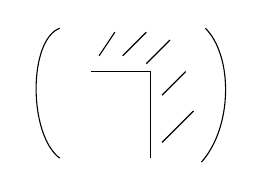
\begin{tikzpicture}
\draw (-0.4,1.05) .. controls (-0.8,0.9) and (-0.8,-0.3) .. (-0.4,-0.6);
\draw (1.45,1.05) .. controls (1.8,0.7) and (1.8,-0.2) .. (1.4,-0.65);
\draw (0,0.5) -- (0.75,0.5) -- (0.75,-0.6);
\draw (0.1,0.7) -- (0.3,1.0);
\draw (0.4,0.7) -- (0.7,1.0);
\draw (0.7,0.6) -- (1.0,0.9);
\draw (0.9,0.2) -- (1.2,0.5);
\draw (0.9,-0.4) -- (1.3,0.0);
\end{tikzpicture}
\end{adjustbox}
\end{center}

$S'_{\mathcal{F}}(M)$, $x\in M$,
$U_x\overset{\text{форм.}}{\longrightarrow}U_0\subset R^N$.

слои слоения $\longrightarrow$ слои форм. слоения.

$S'_{\mathcal{F}}(M)$ — гл. однор. $W_{N,n}$-пр-во!

[Под утверждением две длинные черты, верхняя заканчивается стрелкой вправо.]

$W_{N,n}\supset L$ — сохран. \underline{каждый слой}.
\begin{equation*}
W_{N,n}/L\cong W_n.
\end{equation*}
\begin{equation*}
\begin{adjustbox}{max width=\linewidth}
\begin{tikzcd}
S'_{\mathcal{F}}(M)\arrow[d]\\
S_{\mathcal{F}}(M)
\end{tikzcd}
\end{adjustbox}
\qquad\underline{\text{пост. вдоль слоёв.}}
\end{equation*}
Пара $(S'_{\mathcal{F}}(M),S_{\mathcal{F}}(M))$ —
однородное $(W_{N,n},L)$-пр-во.

\SourcePage{GELFAND-P000394}{39}

[Зачёркнуто: «(формально».]

(факторгруппа не действ. на факторпр-во)
\begin{equation*}
C(W_n)=C(W_{N,n},L)\longrightarrow\Omega(S_{\mathcal{F}}(M)).
\end{equation*}
$S=S_{\mathcal{F}}(M)/GL(n,R)$ — гомот. эквив. $M$.

$(S'_{\mathcal{F}}(M),S)$ — однор. гл. пр-во отн.
$(W_{N,n},L+\operatorname{gl}(n))$.
\begin{equation*}
C(W_n,\operatorname{gl}(n))
=C(W_{N,n},L+\operatorname{gl}(n))\longrightarrow\Omega_M(S).
\end{equation*}
это изв. (образ.) $\psi_1,\dots,\psi_n$ —
Изв. А. Н., 1971, \underline{Гельфанд, Фукс.}

$T(M)/T(\mathcal{F})$ — классы Черна — образы кл. $\psi_1,\dots,\psi_n$.
\begin{equation*}
\prod\psi_i\quad(\text{степ. }>2n)=0.
\end{equation*}
Отсюда для $\underline{T(M)/T(\mathcal{F})}$ произведение кл. Черна
степ. $>2n$ должно быть $0$!! — это теор. Ботта —

— препятствие для сущ. гомотопной интегр.
\Incomplete{GELFAND-P000394}{chern-cancel}{Плотно зачёркнутое слово после «интегр.» не восстановлено.}
$\dots$

\underline{Арнольд.}
\begin{equation*}
\frac{dw}{dz}=\frac{P(z,w)}{Q(z,w)}
\quad\text{на }\underline{CP^2}\setminus\text{неск. особ. точек.}
\end{equation*}
Получ. инвариант слоения (на 3-х мерн. компл. мн-зии: точка — вектор).

Вопрос Арнольда — охарактериз. геометрически,
док. целочисленность (рациональность).

(обобщ. чисел вращ. Пуанкаре).

\underline{Упражнение:} опр. числа вращ. как такой инвариант.
\SourcePage{GELFAND-P000395}{43}
\underline{\underline{14 февраля.}}

\underline{Л. Васерштейн.}

$A$ — ассоц. кольцо с $1$. (не обяз. коммут.).
$V$ — модуль над $A$. (правый).

Квадр. форма над комм. кольцом — в $A^n$ — это
$A^n\longrightarrow A$, запис. в виде $\sum a_{ij}x_ix_j$.
Матрицы опр. неоднозн.

$\exists\,2^{-1}\Rightarrow$ сущ. вз.-одн. соотв. с симм. матрицами.

Инволюция на $A$: $A\longrightarrow A$.
\Incomplete{GELFAND-P000395}{involution-cancelled}{Под стрелкой перечёркнуто короткое слово; видны петли и отдельные штрихи, но целое слово не восстановлено.}
\begin{gather*}
(x-y)^*=x^*-y^*;\qquad (xy)^*=y^*x^*;\qquad (x^*)^*=x.
\end{gather*}
Полуторалин. форма: $f(u,v)\in A$, $u,v\in V$;
аддит. по всем перем.;
\begin{equation*}
\underline{f(u\mu,v\lambda)=\mu^*f(u,v)\lambda}.
\end{equation*}
(см. Бурбаки). (Билин. форм над некомм. кольцом нет)
\begin{gather*}
\operatorname{Hom}(V,V^*)\text{ — это }1{,}5\text{-лин. формы.}\\
V^*=\operatorname{Hom}_A(V,A)\qquad\text{(2-х прав. модулей).}
\end{gather*}
(Hom всегда над $A$).

$V^*$ [зачёркнуто: лев.; прав.; над вторым словом вписано и обведено: лев.]
модуль. (вообще говоря).
\Unclear{GELFAND-P000395}{module-old-adjectives}{Два старых прилагательных перечёркнуты; кандидат «лев.; прав.»; вставленное «лев.» обведено. Второе старое слово пересечено также указателем вставки.}

Но инволюция даёт возм. рассм. $V^*$ как
[зачёркнуто: лев.; выше обведено: прав.] модуль.
\begin{equation*}
a\longmapsto f(a);\qquad \lambda f(a);\qquad a\longmapsto\lambda f(a).
\end{equation*}
$L\in\operatorname{Hom}(V,V^*)$ (гом. прав. $A$-модулей).
\begin{equation*}
f(u,v)=L(u)v.
\end{equation*}

\SourcePage{GELFAND-P000396}{unlabelled}
Квадр. форма — не совсем то.
\Incomplete{GELFAND-P000396}{cancelled-top-word}{Слева перед строкой о кольце густо зачёркнуто слово, начинающееся крупным штрихом; целое слово не прочитано.}
$A$ — кольцо, $*$ — инвол., $\varepsilon\in$ центр $A$,
$\varepsilon\cdot\varepsilon^*=1$.
($\varepsilon$ — симметрия квадр. формы).
(чаще всего встреч. $\varepsilon=1$ или $-1$).

$\Lambda$ — подгруппа аддит. гр. кольца, обл. св-вами:
\begin{gather*}
\{x-\varepsilon x^*\}_{x\in A}\subset\Lambda
\subset\{x=-\varepsilon x^*\}_{x\in A};\\
a^*\lambda a\in\Lambda\quad\text{при }\lambda\in\Lambda\text{ и }a\in A.
\end{gather*}
\Unclear{GELFAND-P000396}{lambda-annotation}{Под «св-вами» справа небольшой незамкнутый скобкообразный штрих и знак, похожий на «э» или «д»; его словесное чтение не установлено.}
Крайние случаи наиболее часто встречаются.

[Зачёркнуто: Т.е.] Кв. формы $\equiv$
полуторалин. на $V$/подгруппа:
\begin{gather*}
X(v,v)\in\Lambda;\qquad X=-\varepsilon X^*,\\
\text{т.е. }X(u,v)+\varepsilon X(v,u)^*=0.
\end{gather*}
[Под «на $V$/подгруппа» наклонная черта к условиям на $X$; горизонтальная разделительная линия.]

По кв. форме $q$ стр. скал. произвед.
\begin{equation*}
(u,v)_q=Q(u,v)+\varepsilon Q(v,u)^*\qquad\text{(линеаризация)}.
\end{equation*}
$Q\in q$; (не зав. от выб. представителя).
Оно — $1/2$-лин. форма.

[Справа в рамке:] $(u,v)_q$ — $\varepsilon$-симметричная форма.
$\varepsilon(v,u)_\varepsilon^*=(u,v)$.

\underline{Отобр. длины:} $\underline{V\longrightarrow A/\Lambda}$.
\begin{equation*}
|u|_q=Q(u,u)+\Lambda.
\end{equation*}
(тоже не зав. от предст.)

$\Lambda\max\Rightarrow$
\Incomplete{GELFAND-P000396}{lambda-max-cancelled}{После стрелки зачёркнуты короткое выражение с q-подобным знаком и фраза с различимыми частями «полуторалин.», «восст.» и предположительным «по квад…»; целиком старый текст не восстановлен.}
квадр. восст. по своим $|v|_q$ (линеар.) и нет смысла различать.

\SourcePage{GELFAND-P000397}{44}
\underline{Пример:} (Гамильтоновы или гиперболические кв. формы)

[Справа обведено:] $A,*,\varepsilon,\Lambda$ — фиксир.

$U$ — $A$-модуль (любой).
$H(U)=U\oplus U^*$ с кв. формой, соотв.
\begin{equation*}
Q(u+f,u'+f')=fu'.
\end{equation*}
\Incomplete{GELFAND-P000397}{sesquilinear-old-prefix}{В скобках перед «1,5 лин.» зачёркнут короткий знак; его первоначальное чтение не восстановлено.}
(1,5 лин.).
\Incomplete{GELFAND-P000397}{hyperbolic-old-matrix}{Под fu' перечёркнута короткая формульная запись с вертикальными и горизонтальными штрихами; её целое выражение не прочитано.}
\begin{equation*}
\begin{pmatrix}0&1\\0&0\end{pmatrix},\qquad
\text{а скал. пр. будет }\begin{pmatrix}0&1\\-1&0\end{pmatrix}.
\end{equation*}
\underline{Группа Витта:} из неособ. форм: т.е.
$(u,v)_q=(L(u)v)$, $L:V\longrightarrow V^*$,
[зачёркнуто: соотв. скал. произв.],
$L$ явл. изоморфизмом.
\Unclear{GELFAND-P000397}{scalar-overwrite}{Первый знак перед (u,v) густо переписан; виден высокий f-подобный штрих поверх более раннего знака. Текущая строка передана как $(u,v)_q=(L(u)v)$; первоначальный знак не установлен.}

\underline{Гр. Витта:}
$(V,q)\perp(V',q')$ — ортог. прям. сумма 2-х мод. с кв. формами
($A,*,\varepsilon,\Lambda$ фикс.).

Неособые кв. формы на конечно порожд.
\Incomplete{GELFAND-P000397}{projective-cancelled}{Между «порожд.» и «проективных» перечёркнут короткий фрагмент; целое чтение не восстановлено.}
проективных модулях. (прям. слаг.,
\Unclear{GELFAND-P000397}{parenthesis-full}{В начале скобок соединённые слова выглядят как «прям. слаг.»; возможны иные чтения средних букв и окончания второго сокращения. Сокращения не развёрнуты.}
\Incomplete{GELFAND-P000397}{parenthesis-cancelled}{После первых двух сокращений в скобках густо перечёркнуто слово; его целое чтение не восстановлено.}
конечномерных свободных).

\underline{Они полугруппа.} Из неё констр. группа (Гротендика),
это и есть гр. Витта.
Над полем есть закон сокращения (теор. Витта).

$K_0O(A)$; $O$ — ортог. $O$ вкл. ($A,*\varepsilon\Lambda$) [снизу: парам.].
Витта—Гротендика.
Витта факториз. по гамильт. [Две вертикальные черты справа.]

[Справа:] \underline{Упр.} $A$ — тело $\Rightarrow$ осн. теор. о сокращ.

\underline{Теор. 1.} $\forall$ конечно пор. проект. мод. с квадр. формой
есть прям. слаг. в гамильт. (кон.-мерн.).
\begin{equation*}
(V,q)\perp\underset{\exists}{\underline{(V',q')}}=H(A^n).
\end{equation*}
\underline{Замеч:} если разреш. сокращ. на $\forall$ мод., то гр. Витта $=0$.
$(a+b+a+b+\ldots)$.

\SourcePage{GELFAND-P000398}{unlabelled}
\underline{Примеры:} \fbox{1} $A$ — поле, $*$ тожд., $\varepsilon=1,-1$
(теор. симм. и
\Incomplete{GELFAND-P000398}{symmetric-cancelled}{Между «и» и следующим сокращением густо перечёркнуто короткое слово; целое чтение не восстановлено.}
симпл. форм.)
Гр. В.-Г. $=Z$.

\fbox{2} $A=Z$, $*$ — тождеств.; $\varepsilon=+1,-1$;
1) $\Lambda=0$ при $\varepsilon=1$;
\Unclear{GELFAND-P000398}{lambda-zero-full}{Между равенством и 0 оставлен высокий перечёркнутый или исправленный знак: наклонная левая сторона, правый стержень и поперечный штрих допускают 4, перечёркнутую единицу, A- или $\Lambda$-подобную старую букву. Текущий кандидат $\Lambda=0$ не восстанавливает старый знак.}
$\Lambda=Z$ или $2Z$ при $\varepsilon=-1$ [под $Z$: 2); под $2Z$: 3)].

1) классифик. квадр. форм: инвар. — ранг и сигнатура (для неособ.).
теор. о сокр. неверна.

2) симплектич.: они изом. \underline{гамильт.}

3) — доп. инвариант — Arf-инвариант.

\fbox{3} Гр. кольцо группы. $A=Z[g]$. Отв. в некот. неизвестны.
$g=Z_p\times Z_q$; неизв. $K_0$.
\Unclear{GELFAND-P000398}{group-index-full}{Последний индекс в $Z_p\times Z_q$ густо переписан и имеет петлю с нижним хвостом. Кандидат q сохранён без восстановления более ранних штрихов.}
Это интер. для топологии (там $\Lambda$ минимально и иногда максимально).

\underline{Взятие Матрицы} над $\underline A$ не меняет $K_0,K_1\ldots$

\underline{Замеч.} (есть неизом. $80\cdot10^6$ кв. форм от 32 перем.)
с $\det=1$.

$K_1O(A)$; $O=(A,*,\varepsilon,\Lambda)$.
$O(H(A^n))$.
\Unclear{GELFAND-P000398}{orthogonal-a-layer}{В $A$ под верхним n два параллельных левых штриха и сгущённая вершина. Текущее A читается; усиление буквы или переписанный A-/ $\Lambda$-подобный слой не разделены уверенно. Прежняя буква не установлена.}
\begin{equation*}
\begin{array}{ccc}&n&n\\n&a&b\\n&c&d\end{array}
\qquad a^*d+\varepsilon c^*b=1;\qquad a^*c\in\Lambda_n\quad(?).
\end{equation*}
[В рукописи блоки a,b,c,d в скобках разделены горизонтальной и вертикальной линиями; n стоит над обоими столбцами и слева от обеих строк.]
(скал. произв. $=1$, а длина $0$).
\begin{equation*}
O(H(A^n))\subset O(H(A^{n+m})).
\end{equation*}
[Зачёркнуто: $O(H(A^\infty))$.] $O(A)$ — их объедин.

\SourcePage{GELFAND-P000399}{45}
\begin{equation*}
O(A)/\underline{[O(A),O(A)]}=K_1O(A).
\end{equation*}
Лемма (Уайтхеда): $[O(A),O(A)]$ порожд. элем. матр.
\begin{equation*}
\begin{pmatrix}1&b\\0&1\end{pmatrix},\qquad
\begin{pmatrix}1&0\\c&1\end{pmatrix}.
\end{equation*}
[Слева под леммой: $EO(A)$. От «(Стейнберг)» наклонная стрелка к $StO(A)$.]
\begin{equation*}
0\longrightarrow K_2O(A)\longrightarrow\underline{StO(A)}
\longrightarrow EO(A)\longrightarrow0.
\end{equation*}
\Incomplete{GELFAND-P000399}{k2-cancelled}{После $K_2O(A)$ перед стрелкой маленький перечёркнутый фрагмент из двух петлеобразных знаков; целое первоначальное выражение не восстановлено.}
[Под $K_2O(A)$: ядро. Под $StO(A)$: универс. центр. накрытие,
расшир. гр. $EO(A)$.]
\begin{equation*}
H_2(G,Z)\longrightarrow\widetilde G\longrightarrow G\qquad([G,G]=G).
\end{equation*}
[Слева наклонная черта.] неприв. система.
\Unclear{GELFAND-P000399}{central-cover-note}{Под строкой $H_2(G,Z)\to\widetilde G\to G$ сокращение выглядит как «неприв. система.»; средние буквы первого слова и его связь с наклонной чертой остаются неоднозначными.}

\underline{Абстр. симплиц. схема.} Симплекс — кон. подмн-во.
мн-во и конечн. подмн-ва и т.д.
\SourceFigure{GELFAND-P000399}{simplex-staircase}{Под словами о множестве и конечных подмножествах длинная ломаная скобкообразная линия: слева короткая верхняя горизонталь, спуск, длинная горизонталь, наклонный спуск, нижняя горизонталь, подъём справа и короткое продолжение вправо. Стрелок и подписанных вершин нет; точная роль ступеней не установлена.}
\begin{equation*}
K_nO(A)=\pi_{n-1}(O(A)).
\end{equation*}
\underline{Симпл. стр. в $O(A)$.}
\Unclear{GELFAND-P000399}{simplicial-overwrite}{Сокращение после «Симпл.» густо переписано; кандидат «стр.»; несколько старых пересекающихся штрихов не разделяются на целую прежнюю запись.}
На конечных $O(H(A^n))$.
[Справа подчёркнуто, линия заканчивается стрелкой влево:]
\begin{equation*}
K_n(A)=\pi_{n-1}(GL(A)).
\end{equation*}
Матр. $(2n)$-го пор.
$\begin{pmatrix}a&b\\c&d\end{pmatrix}$.
Какое кон. мн-во — симплекс?
\begin{equation*}
\begin{pmatrix}1&&*\\&1&\ddots\\0&&1\end{pmatrix}.
\end{equation*}
Любое кон. подмн. в этой подгр. — симплекс.
и прав. и лев. переносы тоже симплекс.
(Все одновр. прив. к $\Delta$ виду).
$K_1$ и $K_2$ ранее опр. совм. с этими.
\Incomplete{GELFAND-P000399}{bottom-cancelled}{Перед нижней строкой слева перечёркнут короткий фрагмент с несколькими буквоподобными штрихами; целое чтение не восстановлено.}
Комм. св-ва. — соотн. элем. матриц.
Трив. соотн. — тоже св. к $\pi_2$.
[Горизонтальная разделительная линия.]

\SourcePage{GELFAND-P000400}{unlabelled}
\underline{\underline{21/II.}}\qquad\underline{\underline{Каждан.}}
\Unclear{GELFAND-P000400}{speaker-full}{После «Ка» узкий соединённый штрих и открытая с-подобная дуга перед высоким д. Возможны «Каждан.», «Каздан.», «Кацдан.» или «Касдан.»; точная фамилия по этим соединённым штрихам не установлена.}

Пусть $A$ — кольцо. Тогда $K_0(A)$ — гр. Грот. проект. $A$-модулей
кон. порожд.; $K_1(A)=GL(\infty,A)/E(A)$.
\begin{equation*}
E(A)=\left\{\begin{pmatrix}1&&*\\&1&\ddots\\0&&1\end{pmatrix}\right\}\text{. подгр.}
\end{equation*}
\Unclear{GELFAND-P000400}{triangular-zero-full}{Нижний левый знак в треугольной матрице густо переписан; кандидат 0. Видны петля, вертикальные штрихи и следы прежнего знака.}
\Incomplete{GELFAND-P000400}{after-subgroup-cancelled}{После «подгр.» отдельно стоит густо зачёркнутый короткий фрагмент; первоначальная запись не восстановлена.}
\begin{equation*}
K_2(A)=\operatorname{Ker}\{St(A)\longrightarrow E(A)\}.
\end{equation*}
(Гр. Гельмгольца—Гротендика — Гельмгольц при изм. цветов — вычит.)
зелёный — жёлтый $=$ синий.

$E_{ij}(a)=$ [матрица], $i\ne j$.
\SourceFigure{GELFAND-P000400}{elementary-position}{В больших круглых скобках несколько единиц по нисходящей диагонали с точками между ними; 0 внизу слева. Справа в верхней части a, над ним вертикальный пунктир и маленькая j-подобная метка; от диагонали к a короткий горизонтальный пунктир. Слева на уровне верхней строки i. Перед скобками знак равенства. Точный размер матрицы и число промежуточных строк не подписаны.}
Гр., порожд. ими, $\underline{\underline{E(A)}}$.

1) $\underline{E_{ij}(a)\cdot E_{ij}(b)=E_{ij}(a+b)}$.
[Окружающие произведение квадратные скобки перечёркнуты; около точки и индекса второго E правка.]
\Unclear{GELFAND-P000400}{relation-full}{В первой строке соотношений скобки перечёркнуты, после E(a) виден зачёркнутый запятообразный штрих около точки; индекс второго E переписан, с небольшими старыми знаками над ним. Кандидат текущей строки $E_{ij}(a)\cdot E_{ij}(b)=E_{ij}(a+b)$ не восстанавливает прежние индексы.}
\Unclear{GELFAND-P000400}{old-e-expression}{Ниже слева перечёркнут незавершённый префикс E с переписанными i-/j-/k-подобными нижними штрихами и открывающей скобкой. После скобки виден незаполненный промежуток; написанного аргумента или продолжения не видно. Точные прежние индексы не установлены.}
\begin{equation*}
(1+ae_{ij})(1+be_{jk})(1+ae_{ij})(1+be_{jk})=1.
\end{equation*}
\Unclear{GELFAND-P000400}{product-full}{В четырёх множителях первые два знака после 1 густо исправлены; кандидаты плюс и минус. Последние два знака выглядят как плюс. В строке оставлены видимые плюсовые кандидаты, без математического исправления результата 1.}
\Incomplete{GELFAND-P000400}{old-result-full}{Под произведением до отдельно написанной 1 зачёркнута короткая запись с различимыми u- или v-подобным и индексоподобным штрихами; целый прежний результат не восстановлен.}
2) $\underline{[E_{ij}(a),E_{jk}(b)]=E_{ik}(ab)}$.
и это все соотношения пока.

В $GL(4,C)$ будет группа матр. с $\underline{\underline{\det=1}}$
порождена элементарными.
т.е. $K_1(A)=C$ для $A=C$;
\Unclear{GELFAND-P000400}{last-field-mark}{Над и справа от последнего C в «A=C» маленький верхний знак, похожий на i или штрих, и отдельная точка ниже; ещё ниже точка с хвостом. Основное C читается; верхняя добавка не определена и не заменена звёздочкой по смыслу.}
и это верно для любого поля.

\SourcePage{GELFAND-P000401}{47}
Рассм. $\{E_{ij}(a)\}$ с указ. соотнош.
(коммут. $a^{-1}b^{-1}ab$).
\Unclear{GELFAND-P000401}{commutator-old-exponents}{Над последними a и b в записи коммутатора зачёркнуты два показателя с минусо- и единицеподобными штрихами. Текущие первые два показателя $-1,-1$ ясны; старые последние показатели целиком не установлены.}
Гр., порожд. ими, наз. $\underline{St(A)}$ (абстр. группа).
(Соотн. в кольце, помимо станд., наз. $K_2(A)$)
Неизв., порожд. ли этими все соотн., верные в любом \underline{\underline{кольце}}.
(все соотн. Steinberg'a).

\Incomplete{GELFAND-P000401}{cancelled-problem-title}{Перед новым заголовком задачи зачёркнута строка; различимы части «Задача» и последнего слова, но вся прежняя формулировка не восстановлена.}
[Слева фигурная скобка объединяет задачу и следующий «Трив. случай».]
\underline{\underline{Задача!!}} (не реш.) — будет ли верное в любом кольце
соотн. следствием стейнберговских?
Трив. случай связ. с нереш. зад. теор. дискр. групп.

$A$, $B=A[t,t^{-1}]$.
$K_0(A)$ — прямое слаг. $K_1(B)$;
$K_1(A)$ — [знак повторения] — $K_2(B)$.

1) $K_0(A)\longrightarrow K_1(B)$.
$K_1(B)$ — автом. своб. модуля.
Будем зад. автом. проект. мод.?
$L\in\operatorname{Aut}P$; $P+Q=A^n$.
[Справа подчёркнуто:] $\underline{L\oplus1\in\operatorname{Aut}A^n}$.
Это корректное опр. в $K_1$.
\begin{equation*}
P[t,t^{-1}]\overset{\mathrm{def}}=P\otimes_A B.
\end{equation*}
[Ниже слева короткий вертикальный штрих.]
\underline{проект. над $B$.}
$P[t,t^{-1}]$ им. автом. — умн. на $t$!
По нему строим
\Incomplete{GELFAND-P000401}{cancelled-before-element}{После «строим» перечёркнуто короткое слово: различимы предположительные «авто» / «авто…», но густая правка перекрывает конечные штрихи; точное целое старое слово и его окончание не установлены.}
элемент $K_1(B)$.

\SourcePage{GELFAND-P000402}{unlabelled}
\underline{Обр. конструкция:}
\begin{equation*}
A^n\longrightarrow(B^n,t)\simeq(B,t^n).
\end{equation*}
Элем. $K_1(B)$ — матрица
$L=\begin{pmatrix}*&*\\\vdots&\vdots\\*&*\end{pmatrix}=t^{-n}L'$,
пор. $r\times r$.
\underline{элем. $L'$ — многочлены!}
\underline{Она обратима в $B$.}
\begin{equation*}
L':A[t]^r\longrightarrow A[t]^r.
\end{equation*}
\Unclear{GELFAND-P000402}{domain-full}{Внутри первых квадратных скобок буква густо переписана, с B-подобной петлёй; кандидат текущего t. Показатель после скобки имеет короткую верхнюю черту и изгиб, кандидат r, возможен n. Старые штрихи не восстановлены по смыслу.}
\Unclear{GELFAND-P000402}{map-old-range}{Перед текущим $A[t]^r$ справа зачёркнуто B-подобное выражение с верхним показателем; кандидат $B^r$ или $B^n$. Показатель густо перечёркнут.}
\begin{equation*}
\operatorname{Coker}L'=A[t]^r\text{-мод.}\Rightarrow A\text{-модули}.
\end{equation*}
\Unclear{GELFAND-P000402}{cokernel-exponent}{В $A[t]^r$ после Coker буква внутри скобок переписана, а верхний показатель r/n-подобен. Формульная строка сохраняет равенство и «-мод.» как в источнике; не заменяется определением коядра.}
Он над $A$ конечно порожд и проективен.
(вроде фредгольм. опер. — конечн. коядра).

$K_2(B)\longrightarrow K_1(A)$.
[Справа:] ($K_1(A)\longrightarrow K_2(B)$) [стрелка вниз: упражн.].

$M=$ [матрица с точками по диагонали и двумя стрелками вдоль неё: вверх-влево и вниз-вправо].
беск. в обе стороны.
В кажд. стр. и ст. конечн. число эл. $\ne0$.
$M^+\subset M$, беск. в одну стор.
\SourceFigure{GELFAND-P000402}{corner-full}{Справа большая пара круглых скобок. В верхнем левом углу внутренний угол из вертикального и нижнего горизонтального отрезков; внутри него несколько наклонных штрихов. Остальная часть скобок не заполнена. Размер и точное число строк не обозначены. Подпись рядом: «заполнен лишь один угол (не фиксир.)».}
заполнен лишь один угол (не фиксир.).
$M_0\subset M^+$.
\Incomplete{GELFAND-P000402}{cancelled-m0-text}{После $M_0\subset M^+$ зачёркнута фраза, в которой видны начальный б-подобный знак и несколько буквенных петель; целая фраза не восстановлена.}
$M\overset{\Psi}{\longrightarrow} M^+/M_0$ — кольцо, гомоморфизм.
[Снизу подчёркивающая линия.]

$M_0$ — кон. число элем. отл. от $0$.
\Unclear{GELFAND-P000402}{m0-extra-exponent}{У M с нижним 0 имеется густо исправленный дополнительный верхний знак, похожий на 0; точное первоначальное положение и чтение знака не установлены.}
[Горизонтальная разделительная линия.]

Влож. $B\overset{\varphi}{\longrightarrow} M$ \underline{\underline{есть.}}
(упражнение на ряд Лорена)
[От M наклонная стрелка вниз-вправо с меткой $\Psi$ к словам:] якобиева матрица.
\Unclear{GELFAND-P000402}{matrix-word}{Первое слово в подписи под стрелкой выглядит как «якобиева»; начальные буквы густо переписаны. Слово сохранено как кандидат без замены названием ожидаемого оператора.}
[Длинная линия над нижними формулами.]
\begin{gather*}
E_{ij}(b_1)\ldots=1\text{ — соотн. эл. матриц. — элемент }K_2\text{ —}\text{нек-рое соотн. (не Стейнберговское).}\\
E_{ij}(\Psi(\varphi(e_i)))\ldots=1.
\end{gather*}
\Unclear{GELFAND-P000402}{argument-full}{В последней строке внутри $\varphi$ буква похожа на e, а индекс на i или 2; кандидаты $e_i$, $e_2$, $b_i$. Она не заменена предыдущим аргументом $b_1$.}

\SourcePage{GELFAND-P000403}{48}
$\ldots M^+/M_0$; «все опер. по вн. непр.»
\begin{gather*}
E_{ij}(\varphi(b_1))\ldots=L.\\
\Psi(L)=1.
\end{gather*}
\begin{equation*}
\begin{adjustbox}{max width=\linewidth}
\begin{tikzcd}
M\arrow[r,"\Psi"]\arrow[dr,"\Psi_1"']&M^+/M_0\\
&M^+\arrow[u,"\Psi_2"']
\end{tikzcd}
\end{adjustbox}
\end{equation*}
$\Psi_2$ — гом. колец; $\Psi_1$ — обрез. — \underline{не гом. колец}.

[Справа отделено двумя вертикальными чертами:]
\underline{Исправление:} надо рассм. матр.,
\Incomplete{GELFAND-P000403}{cancelled-correction-word}{После «матр.» в правой поправке зачёркнуто слово с различимыми в- и р-подобными штрихами; целое чтение не восстановлено.}
к-рые помещаются в конечн. число диагоналей, паралл. главной.
Иначе не гом. колец.
\SourceFigure{GELFAND-P000403}{band-full}{Под правой поправкой в круглых скобках диагонально расположены точки и четыре единицеподобных знака: в нижней части два рядом, выше один и ещё выше справа один. Две диагональные последовательности близки друг к другу; число полных строк, границы полосы и остальные элементы не подписаны.}

Рассмотрим $E_{ij}(\Psi_1(\varphi(b_1)))\ldots=L$.
$L\ne1$, т.к. $\Psi_1$ не гом. колец.
Но $\Psi_2(L)=1$.
$L$ — матр. над $M^+$, отсюда она над $M^0$ — конечная
матр., опр. элем. $K_1(A)$.
[Длинная разделительная линия изгибается вверх к правому полю.]

[На правом поле:] Сем. Бурбаки, докл. \underline{Делиня};
\Unclear{GELFAND-P000403}{bibliography-name}{Фамилия после «докл.» густо переписана и подчёркнута; кандидат «Делиня», возможен «Делинь». Последние штрихи и прежние буквы не отделяются уверенно.}
[В фигурной рамке:] $N=180$, Lect. Notes.
УМН, 1970, $N=3$, Гриффитс.

\underline{\underline{Габриэлов.}}
\underline{Раб.} \underline{Гриффитса} \underline{о вар. структуре Ходжа.}

$X$ — неособое кончн. алг. проект. мн-зие; $\dim X=d$.
\begin{equation*}
H^n(X,Z),\qquad H^n(X,C)=H^n(X,Z)\otimes_Z C.
\end{equation*}
$X$ — кэлерово. На нём есть целочисл. форма $\eta$ второго пор.
типа $(1,1)$.
\begin{equation*}
H^n(X,C)=\bigoplus_{p+q=n}H^{p,q}.
\end{equation*}
$\eta\in H^{1,1}$, замкнута и опр. класс когом.
она задана a priori. $\eta$ наз. \underline{поляризацией}.

\SourcePage{GELFAND-P000404}{unlabelled}
$L:H^n(X,C)\longrightarrow H^{n+2}(X,C)$ — опер. умн. на $\eta$.
\begin{equation*}
\text{Положим }H_0^n=\operatorname{Ker}(L^{d-n+1};H^n\longrightarrow H^{2d-n+2}).
\end{equation*}
примитивные когомологии.
В когом. есть ест. скал. произведение.
Можно док., что $H_0^n$ — ортог. доп. к образу $L$.
\begin{equation*}
H^n(X,C)=\bigoplus L^iH_0^{n-2i}.
\end{equation*}
(разл. Ходжа, Ле Пажа, Лерт и т.д.)
\Unclear{GELFAND-P000404}{decomposition-names}{После «Ходжа» написано «Ле Пажа», затем сокращённая фамилия с началом «Лер» и последним т-подобным штрихом. Кандидат «Лерт» передан без развёртывания или исправления фамилий по теории.}
(т.е. всё разлаг. по примитивным).
$x,y\in H_0^n$.
Рассм.
\begin{equation*}
\Psi(x,y)=(-1)^{\frac{n(n+1)}2}\int_X\eta^{d-n}\Lambda x\Lambda y.
\end{equation*}
\Unclear{GELFAND-P000404}{wedge-full}{Между $\eta^{d-n}$ и x и между x и y два высоких Λ-подобных знака. В строке сохранены Λ; возможна запись клинового произведения крупными знаками, но оно не подставлено по смыслу.}
Это билин. форма — форма Ходжа. [Вставлено снизу и обведено: на $H_0^n$.]

\underline{Свойства:}

1) $\Psi(x,y)=(-1)^n\Psi(y,x)$.

2) $x\in H_0^{p,q}$, $y\in H_0^{p',q'}\Rightarrow\Psi(x,y)\ne0$
лишь в случае $p=q'$, $q=p'$.
\Unclear{GELFAND-P000404}{type-full}{В правой паре равенств q' после p= густо переписано; p' после q= также имеет повторные штрихи. Текущие кандидаты $p=q'$, $q=p'$ сохранены, более ранние буквы не восстановлены.}

3) $0\ne x\in H_0^{p,q}\Rightarrow i^{p-q}\Psi(x,\overline x)>0$.
(в когом. есть компл. сопряжение, $\overline x$ — компл. сопр.)
Пусть $C$ — автом. Вейля — умн. на $i^{p-q}$ в $H^{p,q}$.
(умн. на $i$ в касат. пр-ве).
$\Psi(x,y)$ инв. отн. автом. Вейля.

1) и 3) $\Longleftrightarrow\underline{\underline{\Psi(x,C\overline y)}}$ —
\underline{полож. опр. эрм. форма}.
\SourcePage{GELFAND-P000405}{49}
Осн. идея \underline{Делиня} — можно забыть про мн-зия и оставить
одну структ. Ходжа. Когом. — лин. пр-ва. \underline{Задача лин. алгебры}.
\begin{gather*}
H_{\mathbb Z}\text{ — кон. типа }\mathbb Z\text{-модуль},\\
H_{\mathbb R}=\mathbb R\otimes H_{\mathbb Z};\qquad H_{\mathbb C}=H_{\mathbb Z}\otimes\mathbb C.
\end{gather*}
[Справа, при двойной вертикальной черте:] в прилож. это будут примит. когомологии.
[Зачёркнуто:] \Unclear{GELFAND-P000405}{cancel-hodge}{Вещ. стр.}
$\psi(x,y)$ — билин. форма в $H_{\mathbb C}$ (целоч. — на $H_{\mathbb Z}$ прин. целые знач.).
\underline{Вещ. структ. Ходжа} на $H_{\mathbb C}$ [вставка в обводке: веса $n$] — разбиение
\begin{equation*}
H_{\mathbb C}=\bigoplus_{p+q=n}H^{p,q},\qquad H^{p,q}=\overline{H^{q,p}}.
\end{equation*}
\underline{Поляризация} вещ. стр. Ходжа: задание целоч. $\psi(x,y)$,
инвар. отн. автом. Вейля $C$ ($\psi(Cx,Cy)=\psi(x,y)$) и
$\psi(x,C\bar y)$ — полож. опред. эрмитова форма.
\begin{gather*}
C:\quad H^{p,q}\overset{\times i^{p-q}}{\longrightarrow}H^{p,q},\\
\psi(H^{p,q},H^{p',q'})=0\quad\text{при }p\ne q',\ q\ne p'.
\end{gather*}
Это наз. поляризованной структурой Ходжа.

\underline{27/II}. \underline{Кириллов}. — повторение
\Unclear{GELFAND-P000405}{surname}{Консдана/Констана}.
\begin{gather*}
A\longrightarrow A[t,t^{-1}]=B,\\
K_1=GL(A)/E(A).
\end{gather*}
\begin{center}
\begin{adjustbox}{max width=\linewidth}
\begin{tikzcd}
K_0(A)\arrow[r,shift left]&K_1(B)\arrow[l,shift left]
\end{tikzcd}
\end{adjustbox}
\end{center}
[От $B$ вниз: \underline{ф-ии на надстройке}.]
\begin{equation*}
\underline{M\in GL(B)},\qquad M=t^{-k}\Unclear{GELFAND-P000405}{matrix-cancel}{\text{[зачёркнутый знак]}}M_1.
\end{equation*}
$M_1$ — полин. матрица \Unclear{GELFAND-P000405}{matrix-abbreviation}{мстр.} \underline{$k\times k$}.
\begin{equation*}
A[t]^k\overset{M_1}{\longrightarrow}A[t]^k,\qquad \ker=0.
\end{equation*}
[Справа, при двойной вертикальной черте:]
$\operatorname{Coker}M_1=A$-модуль, к-рый уже конечномерен.
(надо вообще-то разницу между ядром и коядром)
Элем. преобр. не меняют коядра.

\SourcePage{GELFAND-P000406}{unlabelled}
\begin{equation*}
\underline{M=t^{-k}M_1=t^{-\ell}M_2}.
\end{equation*}
[На полях: надо вычесть лишнее.]
[Зачёркнуто: $N$.] \underline{Обр. отображение}.
\begin{gather*}
N\longrightarrow N[t,t^{-1}]\Unclear{GELFAND-P000406}{tensor-relation}{=}N\otimes_A B,\\
N\otimes_A B\overset{t}{\longrightarrow}N\otimes_A B.
\end{gather*}
[Под первым знаком равенства небольшой направленный вниз штрих.]
[Под второй строкой горизонтальная черта.]
дополнить до свободного (иначе не получ. матрицы).
\begin{equation*}
N+M=A^k,\qquad M\otimes_A B\overset{1}{\longrightarrow}M\otimes_A B.
\end{equation*}
Получ. отбр. $B^k\longrightarrow B^k$.
домн. на $t^\ell$, чтобы получ. полиномиальн.?
[Справа: Можно не умножать.]
\begin{gather*}
A^k[t]=M[t]\oplus N[t]\overset{t^\ell\oplus t^{\ell+1}}{\longrightarrow}M[t]\oplus N[t],\\
N[t]\overset{\times t}{\longrightarrow}N[t],\qquad\underline{\operatorname{Coker}=N!!}
\end{gather*}
[В источнике $A^k[t]$ помещено над $M[t]\oplus N[t]$, между ними две вертикальные черты.]
И концы с концами сошлись.
\begin{equation*}
1\longrightarrow K_2(B)\longrightarrow St(B)\longrightarrow E(B)\longrightarrow1.
\end{equation*}
\underline{Swan, Tate}. Два докл. в Nice с [зачёркнуто:
\Incomplete{GELFAND-P000406}{nice-cancel}{слово полностью закрыто густым зачёркиванием}]
разных точек зрения.

\underline{Гельфанд}.
\begin{equation*}
K_0(A)\longrightarrow K_1(B).
\end{equation*}
$N$ — пр. мод.
\begin{equation*}
B\otimes_A(\underset{t}{N}\oplus\underset{1}{M})=A^k.
\end{equation*}
[От равенства вниз: матрица — элем. $K_1(B)$.]
$B^k\longrightarrow B^k$ умн. на $t^{-\ell}$; получ. $A[t]^k\longrightarrow A[t]^k$.
и \underline{Coker}.

\SourcePage{GELFAND-P000407}{50}
\begin{equation*}
0\longrightarrow K_1A\longrightarrow K_1A[t]\oplus K_1A[t^{-1}]
\longrightarrow K_1A[t,t^{-1}]\longrightarrow K_0A\Unclear{GELFAND-P000407}{kzero-detached-mark}{;}\longrightarrow0.
\end{equation*}
\begin{equation*}
K_1A[t]=K_1A\oplus\operatorname{Nil}A.
\end{equation*}
$M:\ A[t]^k\longrightarrow A[t]^k$ обратимая матр. с точн. до элем. преобр.
Для регул. колец \underline{$\operatorname{Nil}A=0$}.
\underline{$K_1A$} — своб. член элем. преобр. экв. к ед. матрице.
Теперь $M=1+tN(t)$; и \underline{обратима}.
можно сделать $N$ не завис. от $t$; $t^2$ разбив. за счёт увелич. пор. матрицы
(свед. к ур-ню 1-го порядка).
\begin{equation*}
1+tN\text{ обр. в многочленах}\quad\Longrightarrow\quad N^k=0.
\end{equation*}
\underline{Nil}$A$ — нильпот. матрицы.
[Разделительная черта.]
\underline{K-функтор по Quillen'у}.
\underline{Morava}. (Колумб. универс.).
\underline{Лемма Квиллена}. (
\Incomplete{GELFAND-P000407}{lemma-parenthesis}{Первое слово в скобках: различимы д…на; предположительно «должна», но целое чтение не установлено.}
\Unclear{GELFAND-P000407}{lemma-following-word}{бы[окончание неясно]} одна из первых в топологии).
$X$ — пр-во, $H$ — норм. подгруппа $\pi_1(X)$, причём $H=[H,H]$;
[на полях, от последнего условия: коммутатор].
Тогда $\exists$ единств. [вставка в обводке: пр-во] $X_H$: (с точн. до гомот.),
\begin{gather*}
X_H=X\cup e^2\cup e^2\cup\dots\cup e^3\cup\dots\cup e^3,\\
\text{таких что}\quad\pi_1(X_H)=\pi_1(X)/H,\\
\text{и}\quad H_*(X,\mathbb Z)\simeq H_*(X_H;\mathbb Z).
\end{gather*}
(кольцо гомологий с целыми коэфф.)
Соотв. функториально по $X$.
\underline{Док-во} с пом. теор. препятствий.

\SourcePage{GELFAND-P000408}{unlabelled}
Пусть $X=BGL(R)$ — классиф. пр-во $GL(\infty)$.
[Под $GL(\infty)$ зачёркнуто:]
\Unclear{GELFAND-P000408}{classifying-cancel}{нед...ная}.
\underline{($R$ — любое кольцо)}.
всё без топологии — \underline{дискр. группа}.
(не имеет ничего общего с Грассм.).
\begin{equation*}
E(R)=[E(R),E(R)].
\end{equation*}
подгр., порожд. элем. матрицами.
\begin{gather*}
\pi_1(BGL(R))=GL(R),\\
\pi_1(X_{E(R)})=GL(R)/E(R)\text{ — его фунд. группа }K_1(R).
\end{gather*}
Теперь $K_i(R)=\pi_i(X_{E(R)})$.
[Зачёркнуто: Неизвестно, верно
\Incomplete{GELFAND-P000408}{kzero-cancel}{средние слова зачёркнутой строки не восстановлены}
при $K_0$.]
$K_0$ надо изменить опр., т.к. $\pi_0(\ )=\{1\}$.
\underline{Квиллен}: если $R$ — поле, то $K_2^{\mathrm{Quillen}}=K_2^{\mathrm{Milnor}}$.
Есть ещё определение \underline{Володина}.
Сущ. теор., применимая к топ. группам. Тогда получ. для $\mathbb R$ и $\mathbb C$ обычн. K-функтор.
\begin{equation*}
K_i(R)(Y)\overset{\mathrm{def}}=[S^i\wedge Y;X_{E(R)}].
\end{equation*}
\SourceFigure{GELFAND-P000408}{suspension}{Под формулой длинная нижняя скобка; от неё короткий штрих к слову «надстройка». Знак между $S^i$ и $Y$ опущен ниже основной строки; точная область, к которой отнесена подпись, не установлена.}
Пробл. Новикова: опр. хар. Черна в алг. K-теории. Здесь свод. к вычисл.
$H_*(X_{E(R)};\mathbb Q)$.

\SourcePage{GELFAND-P000409}{51}
\underline{А. Габриэлов}.
$X$ — алг. проективное мн-зие.
\begin{gather*}
H^n(X,\mathbb C)=\bigoplus_{p+q=n}H^{p,q},\\
F^p=\bigoplus_{\substack{p'>p\\p'+q=n}}H^{p',q}\text{ — фильтрация Ходжа.}
\end{gather*}
\underline{Она двигается голоморфно!}
Будет изуч. повед. этой фильтр., когда $X$ зависит от параметра.
$X_s\subset Y$ — аналит. неособ. мн-зие.
\begin{center}
\begin{adjustbox}{max width=\linewidth}
\begin{tikzcd}
Y\arrow[d,"f"]\arrow[r]&S\times CP^n\arrow[dl]\\
S&
\end{tikzcd}
\end{adjustbox}
\end{center}
[Слева, под $X_s$: вертикальный штрих вниз, ниже $s\in S$.]
[Перед следующими словами зачёркнуто:]
\Incomplete{GELFAND-P000409}{family-cancel}{зачёркнутое слово перед «аналит. отобр.» не восстановлено целиком}
аналит. отобр. (лок. проект.).
$S$ — неособ. алг. проект. мн-зие.
гладкое — лок. тривиальность в анал. смысле.
$O_S$ — пучок анал. ф-ий на $S$;
$f^{\Unclear{GELFAND-P000409}{inverse-symbol}{*}}O_S$ — \underline{теор.-множ. обр.}
[вставлено ниже: \underline{образ.}; изогнутая стрелка к полям: Без тенз. домн-на $O_Y$.]
$R^nf_*f^\circ O_S$ — лок. трив. рассл. со слоем
$H^n(X_s\Unclear{GELFAND-P000409}{fiber-cancel}{\text{[зачёркнутые знаки]}};\mathbb C)$.
[К «рассл.» вставка в обводке: голом.]
[Справа ниже, от области формулы, зачёркнуто:]
\Unclear{GELFAND-P000409}{filtration-cancel}{слоем}.
\underline{в слоях голом. фильтрация расслоениями}.
Относит. компл. де Рама:
\begin{gather*}
\Omega^*_{Y/S},\\
\Omega^1_{Y/S}=\Omega^1_Y/f^*\Omega^1_S;\qquad\Omega^p_{Y/S}=\bigwedge_p\Omega^1_{Y/S},\\
0\longrightarrow f^\circ O_S\longrightarrow O_Y\longrightarrow\Omega^1_{Y/S}\longrightarrow\dots.
\end{gather*}
($f^*O_S=O_Y$, $f^\circ O_S$ — пост. вдоль слоёв).
(резольвента пучка $f^\circ$).
Н. м. $H^{p,q}$ формы от $dz,d\bar z$ движ. не аналитически, т.к. $d\bar z$ преобр. не аналит.
$H^{0,q}$ ясно ($dz$ не входит).
$d\bar z$ остаётся кол-во не увелич. (увелич. голом. часть.
[Последняя скобка в источнике остаётся незакрытой.]

\SourcePage{GELFAND-P000410}{unlabelled}
$S$ — точка, $f^\circ O_S$ — пучок постоянных,
$R^nf_*f^\circ O_S$ — когом., голом зав. от параметра.
(ф-и const на $\forall$ слое, а на $S$ аналитично).
Рассм. спектр. посл. Лерэ:
\begin{equation*}
E_1^{p,q}=R^qf_*\Omega^p_{Y/S}\longrightarrow R^nf_*f^\circ O_S.
\end{equation*}
они индуцируют фильтрацию
\begin{gather*}
R^nf_*f^\circ O_S\supset\mathcal F^p\quad\text{(пучки)},\\
\mathcal F^n=R^nf_*\Omega^0_{Y/S},\\
0\longrightarrow\mathcal F^{p-1}\longrightarrow\mathcal F^p
\longrightarrow E_\infty^{p,n-p}\longrightarrow0.
\end{gather*}
Спектр. посл. вырожд. (все дифф. нулевые).
В рассл. $R^nf_*f^\circ O_S$ есть фильтрация голом. рассл. со слоями $F^p$.
\begin{equation*}
R^nf_*\mathbb C\longrightarrow R^nf_*f^\circ O_S=R^nf_*\mathbb C\otimes O_S.
\end{equation*}
возник. лок. пост. сечения $\Rightarrow$ связность (Гаусса-Манина)
\begin{equation*}
\nabla:\quad R^nf_*fO_S\longrightarrow\Omega^1_S\otimes R^nf_*f^\circ O_S.
\end{equation*}
[Под формулой горизонтальная черта.]

\SourcePage{GELFAND-P000411}{52}
\underline{6/III. М. Ш. Бирман}.
\SourceFigure{GELFAND-P000411}{obstacle-figure}{Вверху слева наклонный сплошной замкнутый овал внутри более широкого прерывистого овального контура. Справа сверху $\Omega$; ниже слева $R$. Справа около контура $u|_{\partial\Omega}=0$. Точное отнесение области $\Omega$ к внутреннему или внешнему контуру не восстановлено.}
$u_{tt}=\Delta u$.
Пусть есть принцип Гюйгенса.
\begin{equation*}
\int_\Omega(|\nabla u|^2+|u_t|^2)\,dx\text{ — сохраняется.}
\end{equation*}
Приход. и уход. решения — не инвар. подпр. с конечной энергией.
$K_+\oplus K_-=\mathcal H\ominus K_0$; (рассм. нач. данные решений).
$K_0$ — реш., эксп убыв. по времени, но сосред. вблизи границы.
$f,\ \left.\frac{\partial f}{\partial t}\right|_{t=0}=f_1$.
Нач. данные — пары $(f,f_1)$ в метрике энергетич.
$K_+$ — расход. волны и при $t=0$ сосред. уже вне сферы рад. $R$.
см. Лакс и Филлипс.
Слова. (ключевые)
\begin{enumerate}
\item Характеристические функции. — 2-х часть кн. Гохберга и Крейна.
\item Рассеяние.
\item «второй лист резольвенты»
\item теория S-матриц.
\item комплексные полюса самосопр. опер.
\end{enumerate}
$H$ близко к $H_0$, если $\forall f\ \exists g_\pm$:
\begin{equation*}
\|e^{-iH_0t}f-e^{-iHt}g_\pm\|\longrightarrow0\quad\text{при }t\longrightarrow\pm\infty.
\end{equation*}
На абс. непр. спектре есть опр. $g_+=U_+f$; $U_+$ — част. изометр.
Пусть весь спектр. абс. непр. Тогда $U_+$ полуунитарен
\begin{equation*}
U_+H_0=HU_+\quad\Unclear{GELFAND-P000411}{intertwining-cancel}{\text{[зачёркнутый знак]}}
\end{equation*}
$H$ сод. часть, унит. эквив. $H_0$.
Задача: когда образ $U_+$ исчерпыв. всё абс. непр. подпр-во $H$?
Это одноканальное рассеяние (на физ. языке).
(т.е. $\exists$ полные волновые операторы).
\underline{многоканальное}: Для опис. $H$ надо $H_0^{(1)},\dots,H_0^{(n)}$,
чтобы образы $U^+$ покрыв. всё пр-во и были ортогональны.
$H_0^{(i)},\ i=1,\dots,n$ — набор опер.; $H$ наз. допуст., если опр. $U_+^{(i)}$

\SourcePage{GELFAND-P000412}{unlabelled}
таковы, что их образы $U_+^{(i)}$ попарно ортогональны. и
\Unclear{GELFAND-P000412}{generate-word}{порожд.} абс. непр. спектр $H$.
\underline{3 частицы} Фаддеев погрузил в схему Лакса и Филлипса.
\underline{Като (1957г)}. $H-H_0$ яд.
$\varphi(H)-\varphi(H_0)\in$ ядерн. Бирман, \underline{1962}.
\begin{gather*}
\underline{S=U_+^*U_-}\text{ — оп. рассеяния},\\
S(\lambda)\text{ — матр. рассеяния (соотв. разлож. }H_0\text{)},\\
S(\lambda)-I_\lambda\in\text{яд.}\quad\text{Бирман — Крейн},\\
\det S(\lambda)=e^{-2\pi i\xi(\lambda)},\\
\operatorname{Sp}[\varphi(H)-\varphi(H_0)]
=\int\frac{d\varphi(\lambda)}{d\lambda}\xi(\lambda)\,d\lambda.
\end{gather*}
(так \underline{опред. $\xi(\lambda)$})
[Разделительная черта.]
\begin{gather*}
D(H)=D(H_0);\\
(H-H^0)E^0(\Delta)\in\Unclear{GELFAND-P000412}{operator-ideal}{\mathcal J_1}
\quad\forall\text{ кон. }\Delta\text{ — дост. для сущ. волн. опер.}
\end{gather*}
Прав. абстр. формулир. — постепенно выделять спектр разных размерностей
(см. \underline{теор. связан. форм} — разные опер. Лапласа).
\underline{О более общем опр. волн. опер.}
\begin{equation*}
U_\pm=\lim_{t\to\pm\infty}e^{iHt}Je^{-iH_0t}.
\end{equation*}
Соотв. разным пр-вам и классич. рассеянию.
\begin{gather*}
1)\quad D(H)=D(H_0),\\
2)\quad(JH_0-HJ)E^0(\Delta)\in\Unclear{GELFAND-P000412}{general-ideal-one}{\mathcal J_1},\\
3)\quad(J^*J-I)E^0(\Delta)\in\Unclear{GELFAND-P000412}{general-ideal-infty}{\mathcal J_\infty}.
\end{gather*}
$J=U_+$ — тривиально есть.
Надо $\approx$ угадать $U_+$.

\SourcePage{GELFAND-P000413}{53}
\underline{Л. Васерштейн}.
Разные K-теории.
1) $A$ — ассоц. кольцо. $K_n=\pi_{n-1}(GL(A))$.
[Справа, при двойной вертикальной черте:] опр. Володина.
опр. абстр. симпл. схемы в $GL(A)$.
$K_1$ совп. с Уайтхедом; $K_2$ с Милнором.
2) Производные функторы (Суон; Герштейн) от $GL$. $K_n^{GS}A$.
Рассм. своб. резольвенту кольца $A$:
\begin{equation*}
A''\longrightarrow A'\longrightarrow A.
\end{equation*}
[Под $A'$ зачёркнуто:]
$\Unclear{GELFAND-P000413}{resolution-cancel}{K_0}$.
[При двойной вертикальной черте:]
$A'$ — своб. [вставлено в обводке: ассоц.] кольцо, порожд. $A$ как мн-вом.
$A''$ — [повторительные штрихи] — [повторительные штрихи] — ядром отобр.
\begin{equation*}
GL(A'')\longrightarrow GL(A')\longrightarrow GL(A)
\end{equation*}
уже не точна..
$K_1$ совпадает (
$\Unclear{GELFAND-P000413}{kone-cancel}{\text{[зачёркнутый знак]}}$
$K_1$ от своб. кольца $=0$).
[На полях, от $K_1$:] матрица, обратимая над своб. кольцом
($\sim$ над любым) есть произв. элементарных.
(Кольца для простоты берутся без единицы).
$A'=\mathbb Z[A]$ — некоммут. многочлены без своб. члена;
[под $[A]$: все эл.]
Производный функтор опр. с пом. симплиц. конструкций.
\begin{gather*}
1\longrightarrow A''\longrightarrow A'\longrightarrow A,\\
K_{n+1}(A)=K_n(A'').
\end{gather*}
(индуктивная ф-ла): опр. всё через $K_1$.
Зад. о соотн. Стейнберга сделана Л. В. и вытекает из совпадения этих K-функторов с Володинскими.
$A$ — кольцо.
$MA$ — матрицы над $A$.
$\Unclear{GELFAND-P000413}{matrix-ring}{\ell}A$ — в $\forall$ стр. и столбце лишь кон. число ненулев. элем.
$MA\longrightarrow\ell A$.

\SourcePage{GELFAND-P000414}{unlabelled}
причём $K_n\ell A=0$! (стягиваемы). [по В. или GS].
($A$ — любое кольцо)
Док-во $\sim$ теор. Койпера.
[Горизонтальная черта.]
\begin{equation*}
MA\longrightarrow\ell A\longrightarrow\mu A\longrightarrow
\Unclear{GELFAND-P000414}{terminal-cancel}{\text{[зачёркнуто: }0\text{?]}}.
\end{equation*}
[Под $MA$ зачёркнуто:
\Incomplete{GELFAND-P000414}{compact-cancel}{зачёркнутое слово под MA не восстановлено целиком}]
аналог комп.
(матр. с кон. числом ненул. элем.)
\begin{gather*}
\underline{K_nA=K_nMA},\\
\underline{K_nA=K_{n+1}\mu A}\quad\text{(из точной последов.)}.
\end{gather*}
Отсюда получ. $K_0$ ($=K_0$ [зачёркнуто:
\Incomplete{GELFAND-P000414}{kzero-cancel}{зачёркнутая фраза внутри скобок перед «обычный» не восстановлена}]
обычный) — полный (своб. модуль $\ne0$).
\begin{equation*}
K_0A=K_{\Unclear{GELFAND-P000414}{shift-index}{1}}\mu A.
\end{equation*}
Отсюда $K_n$ ($-\infty<n<\infty$).
Это совпад. с $K_n$ у Басса.
\begin{center}
\fbox{$\operatorname{Nil}_nA=K_n\,tA[t]$.}
\end{center}
$\forall$ гом. колец соотв. точная послед. $K_n$,
[под «гом.»: $A\longrightarrow B$],
и новое кольцо, так что отн. $K_n=$ абс. от нового кольца.
\begin{gather*}
A\overset{f}{\longrightarrow}B,\\
\dots\longrightarrow K_nA\longrightarrow K_nB\longrightarrow K_nF
\longrightarrow K_{n-1}A\longrightarrow\dots.
\end{gather*}
\SourceFigure{GELFAND-P000414}{relative-figure}{Внизу слева квадрат: обведённое $F$ наверху слева, $\mu B$ наверху справа, $\ell A$ внизу слева, $\ell B$ внизу справа. Стрелки вправо по обеим строкам, вниз по обоим столбцам; справа «влож.». Перед нижней стрелкой густой перечёркнутый знак. От обводки $F$ изогнутая стрелка вниз влево к «универс.». Исходное начертание перечёркнутого знака не восстановлено.}
(расслоенное произвед.; обр. образ)
\underline{pullback}.
По мнению Л. В. теория Квиллена совпадает с этими.
\underline{Теор. Каруби} не совпад.
$tA[t]$ счит. стягиваемым.
\begin{equation*}
\underset{\text{пр-во петель }\Omega A}{t(t-1)A[t]}\longrightarrow tA[t]\overset{t=1}{\longrightarrow}A.
\end{equation*}
\SourcePage{GELFAND-P000415}{54}
\underline{\underline{$K_{n+1}A=K_n\Omega A$.}} По Каруби.

В наст. K-теор. \underline{$K_n tA[t]=Nil$}.

\underline{О теор. Квиллена:}

Пусть $G$ — люб. группа, $E=[G,G]$ и $E=[E,E]$.
Рассм. универс. классиф. пр-во $BG$ с клет. структурой. Publ. Math., 34.
$\pi_1BG=G$, остальные $0$. $(BG=K(G,1))$.

Сдл. Миним. заклейки, превр. в группу (H-пр-во).
Гомологии не меняются. \underline{Убивается $E$}.
Для нового комплекса \underline{$\pi_n=K_n$}.
Всё переносится на \underline{унитарный случай}.

\underline{Теор.} \Unclear{GELFAND-P000415}{theorem-name}{Подчёркнутая фамилия: Валонера / Вагонера; средние буквы соединены.}
\underline{о лорановских расширениях}.
\begin{equation*}
K_2A[t,t^{-1}]=K_2A\oplus K_1A\oplus\text{(обведённый ?)}.
\end{equation*}
\Unclear{GELFAND-P000415}{circled-final-glyph}{Последний обведённый знак имеет 2-подобный верхний изгиб и отдельную нижнюю точку; ? остаётся условным кандидатом, точная природа знака не установлена. Числовое слагаемое не восстановлено.}
теор. верна $\forall n$, но из этого случая следуют все остальные.

\underline{Доказ-во.}
\begin{adjustbox}{max width=\linewidth}
\begin{tikzcd}
A \arrow[r,"\text{своб. член}"'] & A[t,t^{-1}] \arrow[r,"t=1"] & A
\end{tikzcd}
\end{adjustbox}
На правом поле в рамке: \fbox{$K_2$ относит. тривиальна}.
Ниже: \underline{\underline{Умн. на $t$}}. $\in$ центру.

\begin{equation*}
\begin{pmatrix}a&0\\0&a^{-1}\end{pmatrix}
=\begin{pmatrix}1&a-1\\0&1\end{pmatrix}
\begin{pmatrix}1&0\\1&1\end{pmatrix}
\begin{pmatrix}1&\cdot\\0&1\end{pmatrix}
\begin{pmatrix}1&0\\\cdot&1\end{pmatrix}.
\end{equation*}
(ф-ла Уайтхеда).
(точки однозначно восстанавливаются).
\Unclear{GELFAND-P000415}{whitehead-dots}{В третьей матрице верхняя правая запись — точка; в четвёртой нижняя левая — утолщённая точка, 0-подобная. Значения не дописаны.}

$g$ — матр. над $A$. (опр. элем. $K_1$)
\begin{equation*}
\begin{pmatrix}gt&0\\0&g^{-1}t^{-1}\end{pmatrix}
\begin{pmatrix}t&0\\0&t^{-1}\end{pmatrix}
\begin{pmatrix}g&0\\0&g^{-1}\end{pmatrix}.
\end{equation*}
\Unclear{GELFAND-P000415}{matrix-old-t}{Верхняя левая запись средней матрицы переписана: кандидат t, прежний знак не определён; между тремя матрицами знаков равенства нет.}
Теперь их разлож. в элем.; получ. соотнош. — \underline{элем. $K_2$}.

\SourcePage{GELFAND-P000416}{unlabelled}
\underline{Обратное:}
\underline{Элем. $K_2A[t,t^{-1}]$}.
\underline{лор. ряд.} $\rightsquigarrow$ Умн. на него — беск. матрица.
\Incomplete{GELFAND-P000416}{cancelled-upper}{Перед «Получ. соотн.» густо зачёркнута отдельная формула; различимы K-, нижний 2- и A-подобные фрагменты, но формула целиком не восстановлена.}
Получ. соотн. между беск. матрицами.
Обрежем $\Rightarrow$ соотн. $\ell A/\mu A$. (мод. конечн. матриц).
\Unclear{GELFAND-P000416}{quotient-overwrite}{В записи после «соотн.» числитель переписан: читается ℓA, под старым плотным знаком возможно MA; знаменатель μA.}
Нам надо $\ell A/\mu A$. Поднимаем.

\Unclear{GELFAND-P000416}{speaker-heading}{Дважды подчёркнутый заголовок: Каждан / Каздан; соединение после «Ка» неоднозначно.}
\Unclear{GELFAND-P000416}{cancelled-title}{Зачёркнутый заголовок: кандидаты «Пусть есть 2 форм. степ. ряда», «Пусть даны 2 форм. степ. ряда»; второе слово слито с чертой.}
$K$ — поле форм. степ. рядов над $k$ (полем).
Под «степ. рядов» вставлено: (лорана).
$A$ — степ. ряды (Тейлора).
$k\subset K\supset A$.

Пусть
\begin{equation*}
\begin{aligned}
p_1+p_2&=1,\\
p_1A&=0,\\
p_2K&\subset A.
\end{aligned}
\end{equation*}
Справа, отделено двумя вертикальными чертами: $p_i$ — отобр. $K$.
Пусть $f,g\in K$. Вычет \underline{\underline{$f\,dg$}} — ?
\Unclear{GELFAND-P000416}{residue-parenthesis}{После вопроса скобочная помета «без …!»; кандидат «без парам.!» (сокращение сохранено), также прежние кандидаты «без лоран.!», «без полюса!»; соединённые средние штрихи квалифицированы.}
Рассм. $Sp[p_1f,p_1g]$.
\Unclear{GELFAND-P000416}{trace-arguments}{В обоих аргументах после p мелкие нижние знаки: кандидаты 1, 2; первый особенно слит с p.}
Под скобкой с обводкой: опер. конечн. ранга.

\SourcePage{GELFAND-P000417}{55}
13/III.
\underline{\underline{Проф. Morava.}}
\underline{Раб. G. Segal и $K^0$}.

$C$ — катег., $BC$ — симпл. м-во, соотв. этой категории.
точки м-ва — объекты этой категории.
На левом поле: \underline{Гельфанд.}
$C_0$: $[n]=\{0,1,\ldots,n\}$ — объекты вспом. катег.
Морфизмы: $[k]\to[n]$, под стрелкой $\varphi(i)$;
$\varphi(1)\le\ldots\le\varphi(k)$.
\Unclear{GELFAND-P000417}{ordered-map}{В первом аргументе φ видна утолщённая 1; возможен переписанный прежний 0. В строке сохранена 1, не исправлена на 0.}
(см. Габриэль,
\Unclear{GELFAND-P000417}{surname-reference}{Вторая фамилия: Цисман / Цисман с переписанными средними буквами; возможен Зисман.}
)

Обведённое «Контравар.» со стрелкой к следующей строке.
Функтор $A$ из $C_0$ в катег. $K$ наз. симплиц. объектом в кат. $K$.
$A_k$ — образ объекта $[k]$.
$A_0,A_1,\ldots,A_k,\ldots$ и сист. морфизмов.
Если $K$ — кат. множеств, то это
\Incomplete{GELFAND-P000417}{cancelled-prefix-full}{Между «это» и «симплиц.» густо зачёркнуто прежнее короткое слово; целиком не восстановлено.}
симплиц. множество.

\underline{Сист. $A_0$} — м-во точек.
\underline{Сист. $A_1$} — $-\Vert-$ отрезков.
и т. д.
\begin{equation*}
\begin{aligned}
A_0\times\cdot\\
A_1\times\Delta_1\\
A_2\times\Delta_2\\
\ldots
\end{aligned}
\end{equation*}
От нижней записи указатель: станд. симпл.
\underline{и клеим естеств. образом}.
\underline{Получ. наст. комплекс}.

По катег. — симпл. Под строкой длинная стрелка влево.
объекты $C=BC_0$, под строкой волнистая черта.
морф. $BC$.
\SourceFigure{GELFAND-P000417}{bottom-chains-full}{Три горизонтальные строки справа от подписей «1-симплексы», «2-симпл.», «3-симпл.». Первая: надпись BC с нижним 1 над стрелкой a вправо к b-подобной букве. Вторая: три точки со стрелками вправо, снизу a, b-подобная буква, c. Третья: четыре видимые точки с тремя стрелками вправо и ещё стрелка за последней точкой; подписей букв нет. Число и границы последнего продолжения не дополнены.}

\SourcePage{GELFAND-P000418}{unlabelled}
\SourceFigure{GELFAND-P000418}{face-maps}{Вверху справа цепь a→b→c, после c зачёркнут отдельный a-подобный знак. От неё три косые стрелки налево к трём строкам: a→b, b→c, a→c. Под исходной цепью дважды подчёркнуто «3 отобр.». Наложенные штрихи около последнего знака не восстановлены как четвёртая вершина.}
\underline{Пример.}
Если $C$ — один объект,
\Incomplete{GELFAND-P000418}{one-object-old}{После «объект» зачёркнута короткая прежняя запись, целиком не восстановлена; ниже отдельно обведено вставленное e.}
вставлено обведённое $e$;
$\forall$ морфизм — изоморфизм $(C=\text{группа})$.
Под последней скобкой: мн-во морф. $e$.
$BC_1=G$, $Mor(e,e)$.
\begin{equation*}BC_n=G\times G\times\ldots\times G.\end{equation*}
\underline{опред.} $\Rightarrow$ опр. Милнора классифиц. пр-ва
\Incomplete{GELFAND-P000418}{group-old-full}{Перед «группы G» густо зачёркнуто прежнее короткое слово; целиком не восстановлено.}
группы $G$.
т. к. $BC_n\times\Delta_n$ и склеив.
$G$ — топ. гр. $\Rightarrow$ можно \underline{снабдить} топологией.

Пусть $C$ — категория $R$-модулей и изоморфизмов в кат. Мод.
Вставлено ниже: (проективных; конечн. порожд.)
$BC$.
\begin{equation*}
C\times C\longrightarrow C,\qquad (M\times N)\longrightarrow M\oplus N.
\end{equation*}
Знак между $M$ и $N$ переписан поверх прежних штрихов.
\underline{Лемма.} $\alpha,\beta$ — 2 категории $\Rightarrow$
$B(\alpha\times\beta)=B\alpha\times B\beta$.
На левом поле зачёркнуто: Д-во.
\Incomplete{GELFAND-P000418}{product-cancelled}{Справа после формулы произведения густо зачёркнута прежняя фраза; целиком не восстановлена.}
$BC\times BC\longrightarrow BC$; т. е. $BC$ — H-пр-во.

\underline{Замечание.}
\Incomplete{GELFAND-P000418}{remark-cancelled}{После подчёркнутого заголовка зачёркнуто короткое слово; целиком не восстановлено.}
$M\oplus N\ne N\oplus M$ (изом., но не $=$ как объекты катег.)
\begin{adjustbox}{max width=\linewidth}
\begin{tikzcd}
BC\times BC \arrow[r,"\oplus"] \arrow[d,"T"'] & BC\\
BC\times BC \arrow[ur,"\oplus"'] &
\end{tikzcd}
\end{adjustbox}
\underline{некоммут. диаграмма}.
\SourceFigure{GELFAND-P000418}{shuffle-margin}{Справа две вертикальные ограничительные черты переходят в наклонную нижнюю рамку. Внутри: «опред. для симпл. м-в опер.»; верхняя цепь a₁→a₂→…→a₅; вторая b₁→…→b₇, последний нижний индекс переписан. Ниже цепь a₁b₁→a₂b₁→…→a₅b₁→a₅b₂→a₅b₃→…; «всего 12». У правого нижнего поля стрелка вверх, рядом «гомот. коммут.». Порядок цепи и переписанный последний индекс сохранены без дополнительной реконструкции.}

\SourcePage{GELFAND-P000419}{56}
\underline{Замеч.} Если $X\times X\longrightarrow X$ коммут. и ассоциат.
Над строкой в обводке: точно, а не гомот.
$\Rightarrow X\simeq\prod_nK(\pi_n,n)$.
Справа в рамке: Boardman–Vogt, 1968, не опубл.

\underline{\underline{Теор.}} Пусть $X\times X\longrightarrow X$
\Unclear{GELFAND-P000419}{theorem-old-word}{Первое слово после X переписано: кандидат «ассоц.»; первоначальные буквы не отделяются.}
комм. и ассоц. канонич. образом,
Тогда $\exists$ классиф. пр-во;
\Unclear{GELFAND-P000419}{space-old-word}{Первое слово после точки с запятой переписано: «это» / «оно».}
тоже H-пр-во с канонич. гом. коммут. и ассоц. законом.
$BX$ — это классиф. пр-во.
$B(BX)\underset{def}{=}B^2X$.

Слева вертикально:
$C$, $BC$, $B^2C$, $\ldots$, $B^kC$, $\ldots$.
\begin{equation*}
K_C^{-k}(Y)=\lim_{i\to\infty}[Y,\Omega^iB^{k+i}C]_i.
\end{equation*}
\Unclear{GELFAND-P000419}{definition-cancelled}{Между равенством и lim зачёркнута прежняя скобочная запись; видны квадратные скобки и Y-подобная буква, кандидат [Y].}
\Unclear{GELFAND-P000419}{definition-end-full}{После правой квадратной скобки маленькая нижняя i-подобная запись с отдельной точкой; кандидат i, возможен иной добавленный знак.}
Под скобкой, с двумя чертами-связками:
$[S^i\wedge Y,B^{k+i}C]$.
На самом деле
\begin{equation*}B^kC\simeq\Omega B^{k+1}.
\end{equation*}
\Unclear{GELFAND-P000419}{loop-full}{В правой части после B с показателем k+1 буква C отсутствует; это отсутствие сохранено.}
\underline{\underline{$k\ge2$}}, и \underline{предел не нужен}.

\underline{Пример 1.}
$Y=\{*\}$, $C$ — кат. проект. $R$-мод. $\Rightarrow$ K-функтор по Квиллену.
\underline{Пример 2.} $C$ — катег. конечных м-в.
\begin{equation*}BC=\coprod_nB\Sigma_n\end{equation*}
(диз. объед. всех классиф. пр-в симм. групп $\Sigma_n$).
\underline{H-пр-во все вместе}.
Для проект. модулей тоже
\begin{equation*}BC=\coprod_{M\in\text{Proj. мод.}}K(GL(M),1).
\end{equation*}

\SourcePage{GELFAND-P000420}{unlabelled}
Для кат. кон. м-в изв., что
\begin{equation*}K_C^{-k}(Y)=\Pi_s^k(Y).\end{equation*}
(стаб. когомотопич. группы.)
\Unclear{GELFAND-P000420}{stable-index-full}{Нижний индекс при Π переписан и 3-подобен; кандидаты s, 3. Верхний k читается отдельно.}
\begin{equation*}
C=\{\text{кон. мн-ва}\}\longrightarrow\{R\text{-модули}\}=\mathcal R.
\end{equation*}
\Unclear{GELFAND-P000420}{category-letter}{Справа после равенства фигурная R-подобная буква с верхней петлёй; кандидаты каллиграфическая R, ℛ.}
Ниже $k$ точек над фигурной скобкой $k$, стрелка вправо к $R^k$.
\begin{equation*}\Pi_s^k(Y)\longrightarrow K(R)^k(Y).\end{equation*}
$Y$ — точка $\Rightarrow$ или стаб. гом. группы сфер. Получ. их
\Incomplete{GELFAND-P000420}{cancelled-prefix}{В начале следующей строки перед «гомом.» густо зачёркнуто отдельное прежнее слово; целиком не восстановлено.}
гомом. в K-функтор любого кольца.
$R=F_p$, $Y$ — точка ($p$ — простое).
$K(R)^kY$ — образ $j$-гомоморфизма.
\Unclear{GELFAND-P000420}{homomorphism-letter}{Перед «-гомоморфизма» видна нижняя петля j с отдельной верхней точкой; регистр j / J не устанавливается уверенно.}
\underline{След. раз — кобордизмы}. (в том же изложении).

\underline{Васерштейн.}
(для
\Unclear{GELFAND-P000420}{speaker-reference-full}{Фамилия в скобках: Повзнера / Певзнера; первое соединение после П слито.}
).
\Incomplete{GELFAND-P000420}{cancelled-old-definition}{Под заголовком зачёркнуты прежнее начало и строка с K₁, K₀ и словами «новая операция»; начальный Е-подобный штрих передан условно как «Е…», всё прежнее утверждение целиком не восстановлено.}
\underline{Симпл. схема} — мн-во с отмеч. симплексами (конечн. подмн-ва)
(вместе с $\forall$ мн-вом входят все его подмн-ва).
\underline{Топол. пр-во} ему сопоставл. (см. Годеман)
\underline{гомот. группы можно опред. комбинаторно}.

$A$ — любое кольцо; (некоммут.)
$MA$ — конечн. матр. ($\forall$ кон. пор.) (аналог комп. опер.)
$\ell A$ — конечнострочные (в $\forall$ стр. и ст. кон. число эл. $\ne0$)
(аналог огр. опер.)
$\mu A=\ell A/MA$ — кольцо опер. Фредгольма.
$K_iA$.
$GL(A)$ —
\Incomplete{GELFAND-P000420}{cancelled-gl-full}{После GL(A) зачёркнуто прежнее определение; видны начало «обр…» и конечное MA, средняя фраза целиком не восстановлена.}
обр. эл. вида \underline{\underline{$1+MA$}}.
Симплекс — конечн. подмн-во в верхн. треуг. матрицах $\lambda$ и

\SourcePage{GELFAND-P000421}{57}
любое ему сопряж. (дост. с пом. подстановок)
$a_1,\ldots,a_n$ — симпл., если $\exists f,g$ — обр.:
$fa_ig$ — верхн. треуг. (с $1$ на диагонали).
\SourceFigure{GELFAND-P000421}{matrix-size}{Справа небольшая матрица в круглых скобках: три 1-подобные записи вдоль диагонали, звёздочка в верхнем правом углу, C/0-подобная запись в нижнем левом, между последними единицами короткие диагональные штрихи. Конечный размер и нижний левый знак не устанавливаются уверенно; рисунок не развёрнут в полную матрицу.}
В рамке: \fbox{$K_iA=\pi_{i-1}GL(A)$}.
Справа, за двойной вертикальной чертой: Дост. брать сопряж.
\Unclear{GELFAND-P000421}{margin-adjective}{Прилагательное перед «и»: симметричными / сингулярными; кандидат «симметричными» лучше соответствует видимым петлям, слитная середина остаётся неуверенной.}
и
\Incomplete{GELFAND-P000421}{margin-cancelled}{Перед «целоч. матр.» густо зачёркнуто короткое слово; целиком не восстановлено.}
целоч. матр. см. Володин.
\underline{Упражнение:}
\Unclear{GELFAND-P000421}{exercise-word}{Подчёркнутая строка после заголовка: кандидат «найти стрелки»; середина второго слова слитная.}

\underline{\underline{Теорема.}} \fbox{$K_iA=K_{i+1}\mu A$}.
В частности, \fbox{$K_1\mu A=K_0A$}. (индекс). (опр. индекса)
Теор. обобщ. на бан. кольцо $\Rightarrow$ выполн. обычн. теор.
Вопрос для K-функтора Квиллена. А эт
\underline{Это следует из стяг. $\ell A$}. Достаточно \underline{\underline{$K_i(\ell A)=0$}}.
\underline{Стягиваемость $\ell A$} $\Leftrightarrow$ стяг. комплекса $GL(\ell A)$.
(даже в сильном смысле)
\Unclear{GELFAND-P000421}{left-margin-mark}{На левом поле перед зачёркнутым заголовком: наклонный 1-/i-подобный штрих и высокий кривой штрих; точное чтение и функция отметки не установлены.}
\Incomplete{GELFAND-P000421}{cancelled-proof-title}{Зачёркнут заголовок «Док-во стягивания» и отдельная следующая запись; весь прежний заголовок вместе с последней записью не восстановлен.}
В рамке: \fbox{$K_i(\text{своб. кольцо})=0$} —
\Incomplete{GELFAND-P000421}{cancelled-no}{Перед «но стяг.» зачёркнута прежняя короткая запись; целиком не восстановлена.}
но стяг. своб. кольца нет.
\begin{equation*}0\longrightarrow L'\longrightarrow L\longrightarrow A\longrightarrow0.\end{equation*}
Под $L$: своб. кольцо.
\fbox{$K_iA=K_{i-1}L'$}. (сдвиг в другую сторону)
Есть длинный точный послед. (из неё всё следует)
Отсюда следует связь с K-функторами Суона и Герштейна.
($K_0,K_1$ совпад., а дальше индуктивно).
В рамке: $K_i$ с отриц. $i$ есть у Басса — тоже совпадают.
\Incomplete{GELFAND-P000421}{last-cancelled}{В начале последней строки отдельная густо зачёркнутая запись; целиком не восстановлена.}
Для регул. колец все $K_i=0$ с $i<0$.

\SourcePage{GELFAND-P000422}{unlabelled}
\underline{Теор. Каруби:} $i>0$ отлич. от Басса.
Нет делит. нуля — Каруби тоже совпадают.
\underline{Теор. Квиллена:}
\Incomplete{GELFAND-P000422}{cancelled-before-g}{Между заголовком и G густо зачёркнут отдельный старый фрагмент; целиком не восстановлен.}
$G=GL(A)$, $E=E(A)=[E,E]=[G,G]$.
\Unclear{GELFAND-P000422}{equality-full}{Знак после E(A) имеет две горизонтальные черты и нижний косой штрих, кандидат переписанное равенство; возможен прежний знак ≠.}

I. $BG\longrightarrow BG^+$ (постр. Квиллена) и изом. на всех \underline{гомологиях}.
1) на $\pi_1$: $G\longrightarrow G/E$.
(универс. в этом смысле!)
2) со стрелкой к словам «изом. на всех гомологиях».

II. $\exists$ такое $BG^+$, к-рое H-пр-во и универс., т. е. $\forall$ другого отобр. в H-пр-во
\begin{adjustbox}{max width=\linewidth}
\begin{tikzcd}
BG \arrow[r] \arrow[dr] & X\\
& BG^+ \arrow[u]
\end{tikzcd}
\end{adjustbox}
(Morava: и даже без H-пр-в, если индуц. изом.
\Incomplete{GELFAND-P000422}{universal-cancelled-full}{Перед «гомологий» зачёркнуто короткое прежнее слово; целиком не восстановлено.}
гомологий)

Рассмотрим теперь $GL(\mu A)$.
\underline{Стр. Квиллена:}
$K_i^Q A=\pi_iBG^+$, $i\ge1$.
\underline{Теорема:} $K_iA=K_i^Q A$.
\begin{equation*}K_i^Q A=K_i^{S,G,\text{Вол}_1,\text{Вол}_2,\text{Вас}}.\end{equation*}
\underline{Док-во.}
\SourceFigure{GELFAND-P000422}{comparison-full}{Большая сравнительная схема. Верхний левый узел BGL(ℓA), под ним «симплиц.»; справа overline(BGL(ℓA)), ниже «топ. пр-во». Между верхними узлами стрелка вправо. Слева «Действует GL(MA)» и стрелка вниз от верхнего левого узла к BGL(ℓA)/GL(MA); под этим узлом «симпл. сх.». Справа стрелка вниз к overline(BGL(ℓA))/GL(MA), черта над числителем. Между средними узлами стрелка вправо. От левого среднего узла вертикальная стрелка вниз, от правого косая стрелка вниз-влево к общему нижнему узлу overline(BGL(ℓA)/GL(MA)) = BG⁺ !!; черта над всем отношением. Снизу слева «соотв. топ. пр-во», справа «(где G=GL(A))». Начальные B во всех узлах сильно закрашены или переписаны, а верхняя ℓ тоже переписана; возможные старые начальные знаки не определены. Схема описана по геометрии, без восстановления старых букв из конструкции.}

\SourcePage{GELFAND-P000423}{58}
\underline{Утверждение:}
\Incomplete{GELFAND-P000423}{cancelled-top-bar}{Над GL(μA) зачёркнута прежняя короткая запись; видны волнистые остатки букв, целиком не восстановлена.}
$GL(\mu A)=K_0A\oplus\ldots$.
\begin{equation*}
BG=\frac{\overline{GL(\ell A)}}{G=GL(MA)},\qquad
BG^+=\overline{GL(\ell A)/GL(MA)}.
\end{equation*}
\Unclear{GELFAND-P000423}{margin-component}{Справа в рамке: «симпл. схема», черта над всей записью GL(ℓA)/GL(MA), затем «—», маленькая переписанная =/\#-подобная запись с 1-подобным штрихом, «компонента единицы в» и GL(μA) с чертой сверху. Малый знак перед «компонента» не установлен.}
Теорема. В рамке: \fbox{$K_iA=\pi_iGL(\mu A)$}.
В рамке:
\begin{equation*}
\begin{array}{rcl}
H_iGL(\mu A)&=&H_iGL(MA)\\
&&\Vert\\
&&GL(A)
\end{array}
\end{equation*}
\Unclear{GELFAND-P000423}{homology-quotient}{Правая запись имеет HᵢGL(MA) сверху, GL(A) ниже, скобку под верхней строкой и две короткие вертикальные связки. Кандидаты: вертикально поставленное равенство между GL(MA) и GL(A), отношение этих записей; определённая дробь не утверждена. Справа «гомологии как группы», от левой части вертикальная черта вниз к «гомологии её как схемы». Область действия Hᵢ не нормализована по математическому смыслу.}
Поперечная черта через кадр.

20/III.
На левом поле: \underline{Гельфанд.}
\underline{\underline{Теор. Квиллена.}} (доказывается неэлементарно)
$F_q$ — конечное поле; $K_i(F_q)$ — ?
\begin{equation*}
K_0(F_q)=\mathbb Z,\qquad K_1(F_q)=F_q^*.
\end{equation*}
Легко показать, что $K_2(F_q)=0$.
\Incomplete{GELFAND-P000423}{after-k2-mark}{После равенства нулю отдельно густо зачёркнута малая запись; целиком не восстановлена.}
\begin{equation*}
K_{2i+1}(\overline F_q)=\overline F_q^*,\qquad
K_{2i}(\overline F_q)=0,\qquad i=1,2,\ldots.
\end{equation*}
\Unclear{GELFAND-P000423}{closure-odd-full}{Индекс первой группы имеет 2i, утолщённый + и 1; переписанный слой около 2i и + не восстановлен. Кандидат 2i+1 сохранён.}
$\overline F_q$ — замыкание (алг.) поля $F_q$.
(как теор. периодичн.)
\begin{equation*}
K_{2i}(F_q)=0,\qquad K_{2i?1}(F_q)=F_{q^i}^*,\qquad i=1,2,\ldots.
\end{equation*}
\Unclear{GELFAND-P000423}{finite-odd-full}{В нижнем нечётном индексе после 2i и перед 1 плотный переписанный знак; кандидаты +, −. В формуле помещён ?, не выбран знак по теореме.}
\Unclear{GELFAND-P000423}{finite-subindex-full}{В правой части после F нижняя q, у её верхнего правого края отдельная i; кандидат F с нижним qⁱ, возможна иная двухуровневая запись. Формула не заменена на группу заданного порядка.}

\SourcePage{GELFAND-P000424}{unlabelled}
С увелич. $i$ K-функтор прибл. к элементарному K в
\Unclear{GELFAND-P000424}{first-word-full}{Последнее слово первой строки: «замке» / «записи»; средние соединённые штрихи неоднозначны.}
Исп. Автом. Фробениуса.
\underline{Каждан:} \underline{Док-во.}
Рассм. $GL(n,F_q)=G_n$ и её классиф. пр-во \underline{$K(G_n,1)$}.
\Unclear{GELFAND-P000424}{gn-old-index}{Нижний индекс первой записи G переписан, n-подобен; первоначальный знак не установлен.}
$GL(n,F_q)\supset SL(n,F_q)=G_n^0$.
$K(G_n,1)\subset B_n$ —
— «Квиллинизация» $K(G_n,1)$ имеет гомот. группы $=$
$=$ K-функторам кольца.
Цель: сделать фунд. гр. коммут., не меняя групп гомологий.
Заклеиваем коммутант и появившиеся 2-мерные циклы.
Можно огранич. прикл. 3-циклов.

\underline{\underline{Фукс.}}
\underline{\underline{Теор. сущ.}}
$X$ — клет. компл.,
\begin{equation*}
[\pi_1(X),\pi_1(X)]=[\pi_1(X),[\pi_1(X),\pi_1(X)]].
\end{equation*}
Это усл. необх. и дост. для сущ. $Y$ и отобр.
Над $Y$ обведённая вставка со стрелкой: клет.
$f:X\longrightarrow Y$, изом. всех гомологий и
справа в рамке: $1)\ f_*:H_*(X,\mathbb Z)\simeq H_*(Y,\mathbb Z)$.
в $Y$
\Incomplete{GELFAND-P000424}{cancelled-condition-prefix}{Между «в Y» и «2)» зачёркнута прежняя короткая запись; целиком не восстановлена.}
$2)\ \pi_1(Y)$ коммутативно.
Отсюда $\pi_1(Y)$ вычисляется, а именно
\begin{equation*}
\pi_1(Y)=\pi_1(X)/[\pi_1(X),\pi_1(X)].
\end{equation*}
Это теорема существования. Такое $Y$ неединственно.
(Напр., при $\pi_1(X)$ коммут.)
$2\text{а})$ пусть \underline{\underline{$Y$ просто}}
(фунд. гр. действ. на $\pi_n(Y)$ трив.)
Такое $Y$ единственно ($\Rightarrow$ коммут. фунд.-гр., т. к.
$\pi_1$ на себе действ. сопр.) — \underline{теор. Уайтхеда}.
Известно, что H-пр-ва простые.
\SourcePage{GELFAND-P000425}{59}
\underline{Каждан} — \underline{$B_n$ — $H$-пр-во.} (но это не для любой $G$, а для этой).
\begin{equation*}
\underline{K_i(G_n)=\pi_i(B_n).}
\end{equation*}
Квиллен наш. топ. реализ. для $B_n$.

Рассм. катег. [вставлено справа от «катег.»: топ. пр-в; ниже: клет. комплексов],
$X\longrightarrow K^0(X)=[X,BU]$ [к формуле приписано: фактор по трив.].

Опред. опер. Адамса на функторе $K(X)$.

На $U_n$ рассм. ф-ю: $u\longmapsto$
\Unclear{GELFAND-P000425}{eigen-cancel}{неразб. зачёркнутый знак}
собств. зн. $\lambda_1,\dots,\lambda_n$.
\begin{equation*}
\widetilde\psi^k_{\Unclear{GELFAND-P000425}{character-symbol}{\text{зачёркнутый индекс}}}(u)
=\sum_{i=1}^{n}\lambda_{\Unclear{GELFAND-P000425}{power-sum-index}{i}}^k(u)
\end{equation*}
— характер виртуального предст. (разность хар.).

Это предст. $\widehat\psi^k$: $\operatorname{Sp}\widehat\psi^k=\widetilde\psi^k(u)$.

Постр. $\forall$ расслоению другое с действ. $U$ с пом. предст. $\widehat\psi^k$.
Это опер. в $K$-функторе: $\psi^k(\Unclear{GELFAND-P000425}{class-letter}{d})$.
\begin{equation*}
\exists\ \text{отобр. }\psi^k:BU\longrightarrow BU,
\end{equation*}
индуц. опер. Адамса в $K$.
$\Unclear{GELFAND-P000425}{class-letter}{d}\in[X,BU]$,
\Incomplete{GELFAND-P000425}{d-cancel}{После формулы зачёркнут фрагмент: видны ψ-подобное начало и круглый штрих ближе к концу; внутренний остаток под штриховкой не восстановлен.}

\begin{equation*}
(\psi^k\Unclear{GELFAND-P000425}{fiber-map-sign}{-}1):BU\longrightarrow BU.
\end{equation*}
[Справа вставка в контуре: «превращ. в», остриё контура к слову «расслоение».]
\Incomplete{GELFAND-P000425}{bundle-cancel}{Перед словом «расслоение», под вставкой, целый зачёркнутый фрагмент не восстановлен.}
расслоение.
\SourceFigure{GELFAND-P000425}{vertical-figure}{Справа два BU друг под другом, между ними толстая стрелка вниз; слева от стрелки записано ψ в степени k минус 1, справа на уровне стрелки — Eψ в степени k. Слева выше верхнего BU небольшой зачёркнутый знак. Связь боковой надписи Eψ с вертикальной стрелкой отдельно не обозначена.}

$E\psi^k$ — слой отобр. $\psi^k-1$.

\underline{Утв.:}
\underline{$E\psi^{\Unclear{GELFAND-P000425}{fixed-statement}{k}}=B_n=B$}
при большом $n$.

Автом. Фробениуса $\sim$ опер. Адамса в топ.

\underline{Другое опред.} [сверху справа: $\Unclear{GELFAND-P000425}{definition-heading-mark}{k}$].

Пусть $[K(X)]^k\subset K^0(X)$,
\begin{equation*}
[K(X)]^k=\{\Unclear{GELFAND-P000425}{class-letter}{d}\in K^0(X)\mid
\psi^k\Unclear{GELFAND-P000425}{fixed-equality}{\text{зачёркнутый знак}}\Unclear{GELFAND-P000425}{class-letter}{d}=\Unclear{GELFAND-P000425}{class-letter}{d}\}.
\end{equation*}
он представим и
\begin{equation*}
[K(X)]^k=[X,E\psi^k]
\end{equation*}
\underline{легко проверить.}

\SourcePage{GELFAND-P000426}{unlabelled}
$K(G,1)\subset B$. Отожд. $B$ с $E\psi^q$.

[Зачёркнуто:]
$\Unclear{GELFAND-P000426}{top-cancel}{[K(X)]^{\text{неразб.}}\ \text{и правый знак}}$.

Рассм. $GL(n,F_q)$ и фикс. гомом. $\mu:\overline F_q^*\longrightarrow C^*$.

На $GL(n,F_q)$ постр. ф-ю — характер представл.
\begin{equation*}
\underline{\varphi_\mu(g)=\sum\mu(\lambda_i),}
\end{equation*}
где $\lambda_i$ — соб. зн. матр. $g$.

Надо постр. отобр. $K(G_n,1)\longrightarrow E\psi^q$ или элем.
$[K(G_n,1),E\psi^q]$, т.е. элем. $K$-функтора от $K(G_n,1)$,
инвар. относит. $\psi^q$,
\Incomplete{GELFAND-P000426}{invariance-cancel}{После указания инвариантности целый фрагмент зачёркнут и закрыт штрихами.}
Дост. задать представление группы $G_n$ (тогда получ. элем. $K(K(G_n,1))$. [Открывающая скобка перед «тогда» в источнике не закрыта.]

Из теор. \underline{Брауэра} [вставка в контуре: $\Unclear{GELFAND-P000426}{brauer-insert-symbol}{\psi}_\mu(g)$]
\Incomplete{GELFAND-P000426}{brauer-cancel}{Под вставленной формулой густо зачёркнута короткая запись; исходный текст под чертами не восстановлен.}
— характер вирт. представления.

Набор $\lambda_i^q$ — тоже соб. знач. — те же $\Rightarrow$ инвариантность.

На \underline{$E\psi^q$} есть структ. $H$-пр-ва $\Rightarrow$
отобр. прод. до отобр. в $B_n$ (на затянутые диски).

Другой способ: $SL$ порожд. унипот. матрицами и их и нужно затягивать
$\Rightarrow$ а на них $\varphi_\mu=1$.

Гомот. гр. $E\psi^q$ из
\begin{center}
\begin{adjustbox}{max width=\linewidth}
\begin{tikzcd}
&B_n\arrow[dr,"\sim\text{ — гомот. эквив.}"]&\\
K(G_n,1)\arrow[ur]\arrow[rr]&&E\psi^q
\end{tikzcd}
\end{adjustbox}
\end{center}
\SourceFigure{GELFAND-P000426}{small-figure}{Справа от слов о гомотопических группах: BU вверху и BU внизу, стрелка вниз между ними; справа от стрелки Eψ в степени q. Не указано, является ли правая надпись меткой стрелки или отдельным объектом.}

У $E\psi^q$ гомологии счит., а у $B_n$ — ?

Гр. гомологий \underline{$K(G_n,1)$} считаются (тоже Квиллен)
с примен. étale-топологии (см. Annals).
\begin{equation*}
\varphi:G\longrightarrow G,\qquad
\varphi(g)=g^{-1}g^\sigma
\end{equation*}
($\sigma$ — автом. Фробениуса).

Теперь пишем спектр. посл. рассл. и счит.

[Справа внизу, отделено двумя вертикальными чертами:]
\underline{След. раз:} кобордизмы.

\SourcePage{GELFAND-P000427}{60}
\underline{М.Ш. Бирман.}\quad \underline{Теор. Като.}

$H-H_0\Unclear{GELFAND-P000427}{upper-relation}{=}V\in\Unclear{GELFAND-P000427}{operator-ideal}{\gamma_1}$
(ядерный опер.).

Док., что абс. непр. части $H$ и $H_0$ унит. эквив.
$H,H_0$ — самосопряженны.

[На правом поле сверху: $\Unclear{GELFAND-P000427}{upper-right-mark}{f}$.]

\underline{Вопрос} (И.М. Гельфанд): как по набору спектр. типов можно
устан., реализ. ли они так, чтобы разность была ядерным опер.

Спектр в факторкольце по ядерным — ?

\underline{2 факта использ.:}

1) $D_1,D_2\in\Unclear{GELFAND-P000427}{operator-ideal}{\gamma_2}$;
$E_\lambda$ — разл. единицы $\Rightarrow$
\begin{equation*}
\Rightarrow\frac{d}{d\lambda}D_1E_\lambda D_2
\end{equation*}
почти всюду сущ. и ядерно ($\sim$ теор. об оснащ.).

(см. Гельфанд, дифф. ф-ла сильно огр. вар.)

2) $D_1R_zD_2\longrightarrow D_1R_{\lambda+i0}D_2$ почти всюду в
$\Unclear{GELFAND-P000427}{operator-ideal}{\gamma_2}$.

Оператор, осущ. унит. эквив.:
\begin{equation*}
\left.
\int_{-\infty}^{\infty}\frac{d}{d\lambda}
(E_\lambda(I+VR_z^0)f,g)
\right|_{z=\lambda\pm i0}d\lambda=(W_\pm f,g).
\end{equation*}
($V$ разбиваем в 2 гильб.-Шм.)

Будет в след. раз.

\underline{27/III}\quad \underline{Каждан.}

\underline{Теор. Артина–Мазура.}

Если $X$ — мн-зие над полем $k$ [над $k$ вставлено: «любым!!»],
по нему можно постр. комплекс $C_X$.

Если $k=C\Rightarrow C_X=\widehat X_C$ — \underline{пополнение}.

Алгебр. постр. $\longrightarrow$

$\longrightarrow$ (автом. поля $k$, сохр. $X\sim\longrightarrow$
\Incomplete{GELFAND-P000427}{bottom-cancel}{Перед $C_X$ зачёркнут короткий фрагмент: начальные не-подобные следы различимы, внутренний остаток под чертами не восстановлен; снизу вставлено «действ. на».}
$C_X$) [под зачёркиванием вставлено: «действ. на»].

Если $X$ опр. над $Q$, то $\operatorname{Gal}(C\mid Q)$ действ. на $C_X$.

\SourcePage{GELFAND-P000428}{unlabelled}
Пусть $X$ —
\Incomplete{GELFAND-P000428}{top-cancel}{После «Пусть X —» зачёркнуто сокращение: видны частичные мн-/мн-ие-подобные следы; внутренний остаток под чертами не восстановлен.}
[вставка в контуре: «топ. пр-во.»].

Рассм. функтор [две вертикальные черты] $X\longrightarrow X_i$
[снизу волнистая черта и слово «категория»].

образы всех $\pi_n(X)$ — кон. группы.

$\forall Y$ рассм. мн-во $\underline Y\longrightarrow X_i$:
$\prod_i\operatorname{Hom}(\underline Y,X_i)$,
и согласов. $\underline{h_{\widehat X}(Y)}$ — функтор.
Он представим и $\widehat X$ — предст. объект.

\underline{И.М. Гельфанд.}
\underline{Станд. язык.}

$1^\circ$. Категория и функтор (Гротендик «О нек. вопр. гом. алг.» — 1 глава).

$2^\circ$. Topos (топо́). $+$ теор. о
\Unclear{GELFAND-P000428}{descent-word}{спуске}.

(опред. есть в предисл. Манина к ст. \underline{Мамфорда})

M. Artin — Grothendieck.

\underline{М.Ш. Бирман.}\quad \underline{Теорема Като.}

$\Unclear{GELFAND-P000428}{hilbert-symbol}{\mathfrak H}$ — гильб. пр-во.
$H,H^0$ — опер., $H-H^0\in\Unclear{GELFAND-P000428}{middle-class}{\gamma_1}$.
\begin{equation*}
e^{iHt}e^{-iH^0t}P^0
\end{equation*}
$P^0$ — проектор на абс. непр. подпр. $H^0$.
\begin{equation*}
\underset{t\to\pm\infty}{s\text{-}\lim}e^{iHt}e^{-iH^0t}P^0=W_\pm.
\end{equation*}

Тогда и $W_+$ и $W_-$ задают изом. абс. непр. спектров $H$ и $H^0$
(симметрия предположений!)

\begin{equation*}
W_\pm H^0=HW_\pm.
\end{equation*}
[Под равенством скобка; справа двойные вертикальные черты и угловая скобка к заметке об области изометричности.]

$P^0\Unclear{GELFAND-P000428}{hilbert-symbol}{\mathfrak H}$ —
обл. изометричности $W_\pm$ (на доп. он $0$).

\underline{Обл. значений:} совп. ли она с подпр-вом
$P\Unclear{GELFAND-P000428}{hilbert-symbol}{\mathfrak H}$?
[Под последней записью угловая скобка.]

\SourcePage{GELFAND-P000429}{61}
\underline{Предл.}
Обл. знач. $W_+$ совп. с $P\Unclear{GELFAND-P000429}{hilbert-glyph}{\mathfrak H}$
$\Leftrightarrow\exists$ волн. опер. $W_+$ с перем. ролей $H$ и $H_0$.

Отсюда существование $\Rightarrow$ полнота из сим. соотн.
\begin{equation*}
W_\pm(H_3,H_2)\underline{W_\pm(H_2,H_1)}
=\underline{W_\pm}(H_3,H_1).
\end{equation*}
\underline{Док-во теор.:}
\begin{equation*}
\left.\int_{-\infty}\frac{d}{d\lambda}
(E_\lambda(I+VR_z^0)f\Unclear{GELFAND-P000429}{first-integral-argument}{\text{зачёркнутый знак}},g)
\right|_{z=\lambda\pm i0}d\lambda=(W_\pm f,g).
\end{equation*}
Это опред. билин. формы этого опер.;
\underline{Надо уметь:} $\frac{dE_\lambda g}{d\lambda}$,
а это можно при $\frac{dDE_\lambda g}{d\lambda}$,
где $D$ — опер. Г.-Ш.

Произв. \Unclear{GELFAND-P000429}{literal-density-word}{составляет} сразу абс. непр. часть спектра.

Факториз. $V$ в $2$ опер. Г.-Ш.

Почти всюду сущ. произв. $(E_\lambda f,g)$.
\begin{equation*}
\frac{d(E_\lambda f,g)}{d\lambda}
+\left(D_1R_{\lambda+i0}^0f,\frac{dD^*E_\lambda g}{d\lambda}\right)
\end{equation*}
\begin{equation*}
V=D_{\Unclear{GELFAND-P000429}{factor-index}{2}}D_1;
\qquad D_i,D\text{ — опер. Г.-Ш.}
\end{equation*}
Опер. $W_\pm$ не зав. от разл. $V$ в произв.
\begin{equation*}
R_z^0-R_{\bar z}^0=Q_z^*(R_z-R_{\bar z})Q_z;
\qquad Q_z=I+VR_z^0.
\end{equation*}
Далее,
\begin{equation*}
\frac{d(E_\lambda^0f,g)}{d\lambda}
=\left.\frac{d}{d\lambda}
\left(E_{\Unclear{GELFAND-P000429}{last-density}{\lambda}}
Q_{\mu\pm i0}f,Q_{\mu\pm i0}g\right)\right|_{\mu=\lambda}.
\end{equation*}

\SourcePage{GELFAND-P000430}{unlabelled}
Все $D$ — нужные оснащения.

см. статью в «Известиях», 1967г.
\begin{equation*}
\left.\int_{-\infty}^{\sigma}\frac{d}{d\lambda}
(E_\lambda(I+VR_z^0)f,g)\right|_{z=\lambda\pm i0}d\lambda
=(E_\sigma W_\pm f,g).
\end{equation*}
\underline{Более общ. вар.:}
\begin{equation*}
E(\Delta)(H-H^0)E^0(\Delta)\in\Unclear{GELFAND-P000430}{upper-class-symbol}{\gamma_1}.
\end{equation*}
$D(f(H))=D(f^0(H^0))$, $f,f^0$ на беск. растут.

\underline{3/IV–72г.}\quad \underline{Минимум.}

1. Топ. Гротендика и производные функторы.

2. Спуск.

3. \Unclear{GELFAND-P000430}{middle-agenda-third}{Симплиц.}

\underline{Экзамен:} разобрать ст. Артина о связи форм. и алгебр. объектов.

\underline{Геронимус.} [Под именем толстая заштрихованная полоса.]

\underline{Опр. Топологии Гротендика.}

кат. $T$ каждому $X\ni T\overset{\text{сопост.}}{\sim\longrightarrow}\operatorname{Cov}_T X$ — мн-во,
его элементы $\{f_\alpha:X_\alpha\longrightarrow X\}$
(сем-во морфизмов). ($\alpha\in A$ — мн-во).

1) $f:Y\longrightarrow X$ изом. в кат $T$.
Тогда $\{f:Y\longrightarrow X\}$ покрытие.

2) $\{f_\alpha:X_\alpha\longrightarrow X\}\in\operatorname{Cov}_T X$
и $\forall\alpha$ зад.
$\{f_{\alpha\beta}:X_{\alpha\beta}\longrightarrow X_\alpha\}
\in\operatorname{Cov}_T X_\alpha$.

Тогда
\begin{equation*}
\{f_\alpha\circ f_{\alpha\beta}:X_{\alpha\beta}\longrightarrow X\}
\in\operatorname{Cov}_T X.
\end{equation*}

\underline{Мамфорд, Математика 13:2}

3) $\{f_\alpha:X_\alpha\longrightarrow X\}\in\operatorname{Cov}_T X$,
$f:U\longrightarrow X$ — произв. морф.

\SourcePage{GELFAND-P000431}{62}
Тогда $\Unclear{GELFAND-P000431}{top-mark}{\text{зачёркнутый знак}}$

3.1 $X_\alpha\times_X U$ сущ. (рассл. произв.)

3.2 $\{p_2:X_\alpha\times_X U\longrightarrow U\}\in\operatorname{Cov}_T U$.

\underline{Опр. рассл. произв.:}
\begin{center}
\begin{adjustbox}{max width=\linewidth}
\begin{tikzcd}
&Z\arrow[dl,"p_1"']\arrow[dr,"p_2"]&\\
U\arrow[dr,"f"']&&V\arrow[dl,"g"]\\
&X&
\end{tikzcd}
\end{adjustbox}
\end{center}
$Z$ универс. — рассл. произв.

$T$ — исх. категория.

Пусть $A$ — фиксир. абелева категория (с беск. прям. суммами)

Предпучок:
\Incomplete{GELFAND-P000431}{presheaf-cancel}{Между двоеточием и «контравар.» зачёркнуто целое слово, закрытое штрихами.}
контравар. функтор из $T$ в $A$: $F:T^0\longrightarrow A$.

$P_T$ — категория предпучков.

Он наз. пучком, если $\forall$ покрытия послед.
\begin{center}
\begin{adjustbox}{max width=\linewidth}
\begin{tikzcd}
0\arrow[r]&F(X)\arrow[r,"\bigoplus F(f_\alpha)"]&
\bigoplus_\alpha F(X_\alpha)\arrow[r,shift left,"F(p_1)"]
\arrow[r,shift right,"F(p_2)"']&
\bigoplus_{\alpha,\beta}F(X_\alpha\times_X X_\beta)
\end{tikzcd}
\end{adjustbox}
\end{center}
\underline{$S_T$ — полная подкатег. пучков в кат. предпучков}

\underline{Морфизм функторов.}
$F:C\longrightarrow D$, $G:C\longrightarrow D$,
$F\overset{t}{\longrightarrow}G$.

$\alpha:C_1\longrightarrow C_2$,
\begin{center}
\begin{adjustbox}{max width=\linewidth}
\begin{tikzcd}
F(C_1)\arrow[r,"F(\alpha)"]\arrow[d,"t(C_1)"']&
F(C_2)\arrow[d,"t(C_2)"]\\
G(C_1)\arrow[r,"G(\alpha)"']&G(G_2)
\end{tikzcd}
\end{adjustbox}
\end{center}
Это глубокое понятие. Нетривиальность: много разных $\alpha$,
а $t(C_i)$ ровно $2$.

\SourcePage{GELFAND-P000432}{unlabelled}
Отсюда сами функторы образуют «категорию».

(с точностью до того, что морф. могут не образов. мн-во)

[Зачёркнутая формула:]
\SourceFigure{GELFAND-P000432}{top-cancel}{Зачёркнутая короткая запись: слева Y-подобный знак, справа A-подобный знак, между ними стрелка вправо. Длинные вертикальные зигзагообразные штрихи пересекают запись; оба буквенных чтения остаются кандидатами.}

\underline{Теорема:}\quad \underline{категория $S_T$ — абелева.}

$i:S_T\longrightarrow P_T$ (функтор).
[Под $P_T$ вертикальная черта к подписи: \underline{кат. предпучков}.]

\underline{Идея док-ва:}

$\exists$ функтор $\# :P_T\longrightarrow S_T$, сопряж. к \underline{$i$}.

(ассоциир. пучок).

\underline{Функторы:}
$F:T_1\longrightarrow T_2$,
$G:T_2\longrightarrow T_1$
наз. сопряж., если $\forall X\in T_1$ и $\forall Y\in T_2$
зад. ест. изоморфизм
\begin{equation*}
\operatorname{Hom}(X,GY)\cong\operatorname{Hom}(FX,Y).
\end{equation*}
[Под каждым из двух Hom дуга и стрелка вниз к надписи:]
изом. $2$-х функторов из произв. их категорий из катег. множеств.

[Справа на поле, отделено двумя вертикальными чертами:]
\underline{Опр.} с пом. универс. морф. предп. в пучок тоже годится.

(\underline{изом.} функторов — см. $1$-я гл. Гротендика).

[От подчёркнутого «изом.» черта вниз к следующему:]
$\exists$ $2$ морф. функторов, такие что композ. тождеств.

(док-во см. Артин).

\SourcePage{GELFAND-P000433}{63}
\underline{Определение.}
Пусть $T$, $X\in T$, $F\in S_T$.
\begin{equation*}
H^q(T,X,F)\overset{\mathrm{def}}=R^qi(F)(X).
\end{equation*}
$R^qi$ — новый функтор (тоже из $S_T$ в $P_T$).

[Зачёркнуто:
\Unclear{GELFAND-P000433}{cancelled-sentence}{Берётся его знач. на объекте $X$; конечные штрихи неясны}.]

Его знач. на $F$ — предпучок (т.е. тоже функтор).

Предпучок на $X$ —
[Зачёркнуто: \Unclear{GELFAND-P000433}{presheaf-cancel}{это}.]
. . . . .

\underline{Определение.}

$f:T_1\longrightarrow T_2$ морф. топ.
$\underset{\mathrm{def}}{\Leftrightarrow}$ покрытие $\longrightarrow$ покр.

$f^*:S_{T_2}\longrightarrow S_{T_1}$ (тоже функтор).
\begin{equation*}
f^*F(X)=F(f(X)),\quad\text{где }X\in T_1,\ F\in S_{T_2}.
\end{equation*}
\underline{Легко пров., что это пучок.}

\underline{Спектр. послед. Лерэ.}

$f:T_1\longrightarrow T_2$; $X\in T_1$; $F\in S_{T_2}$.

Тогда сущ. спектр. послед. со $2$-м членом
\begin{equation*}
E_2^{p,q}=H^p(T_1,X,R^qf^*(F))\Rightarrow H^*(T_2,f(X),F)
\end{equation*}

Пусть $A,B,C$ — аб. категории
\begin{equation*}
A\overset F{\longrightarrow}B\overset G{\longrightarrow}C.
\end{equation*}
Тогда (при изв. усл.) сущ. спектр. послед
\begin{equation*}
R^pG\circ R^qF(X)\Rightarrow R^*(G\circ F)(X)
\end{equation*}
Теор. Лерэ — частн. случай этой ситуации: $\Rightarrow$

\SourcePage{GELFAND-P000434}{unlabelled}
[Зачёркнутая формула:]
$\Unclear{GELFAND-P000434}{cancelled-identity}{i_{T_2}f(X)=f^*\circ i_{T_1}(X)}$.

\begin{equation*}
i_{T_2}f_s^*F=f_p^*\circ i_{T_{\Unclear{GELFAND-P000434}{live-right-index}{1}}}F
\end{equation*}
[Под формулой открытая сверху скобка: нижняя горизонталь с вертикальным концом слева и справа.]
— тождество (тавтология).

$f_p^*$ — тот же морф. на предпучках.

Теор. Лерэ есть частн. случай, т.к. $f_p^*$ точен в кат. предпучков.

[Слева зачёркнуто:]
$\Unclear{GELFAND-P000434}{left-cancel}{\text{неразб. знак}}$.

\underline{Классифицирующая топология.}

\underline{Определение.}
Пусть $T$ — \Unclear{GELFAND-P000434}{topology-word}{топ.} Гротендика,
$G$ — группа в кат. $T$.
\begin{equation*}
X\in T\sim\longrightarrow h_X:T^0\longrightarrow\operatorname{Ens}
\end{equation*}
(контравар.)
\begin{equation*}
h_X(Y)=\operatorname{Hom}(Y,X).
\end{equation*}
Вместе с $G$ должна быть зад. структ. группы в \underline{$h_G(Y)$},
функториальная по $Y$ и
\begin{equation*}
h_G(Y_1)\overset{h_G(\alpha)}{\longrightarrow}h_G(Y_2)
\end{equation*}
есть гом. группы. ($\alpha:Y_2\longrightarrow Y_1$).

\underline{Другое опр.:} совок. $3$-х морфизмов
\begin{gather*}
G\times G\longrightarrow G\\
G\longrightarrow G\\
e\longrightarrow G.
\end{gather*}
($e$ — финальный объект в катег.)

связ. неск. коммут. диагр.

$G$ действ. на $X$, если $\forall Y\in T$:
\begin{equation*}
h_G(\Unclear{GELFAND-P000434}{final-action}{Y})
\text{ действ. на }
h_{\Unclear{GELFAND-P000434}{final-action}{X}}(Y).
\end{equation*}
[Под формулой угловая скобка:] функт. по $Y$.

[Слева вставка в контуре, соединена длинной изогнутой стрелкой с «$G$ действ. на $X$»:]
\underline{$X$ — $G$-объект} [в отдельном маленьком контуре: «слева»].

\underline{$TG$} — новая топ. Гротендика. Категория —
\SourcePage{GELFAND-P000435}{64}
— $G$-множества ($G$-объекты).

$X\in T$ и на нём действие $G$.

Объекты [зачёркнуто:
\Incomplete{GELFAND-P000435}{objects-cancelled}{Короткая запись между «Объекты» и «кат.» закрыта плотным зачёркиванием; целиком не прочитана.}]
кат. $TG$ — $G$-объекты.

Морф. — коммут. с действием ($G$-морфизмы).

Покрытия — те покр. $\underbrace{\{f_\alpha:X_\alpha\to X\}}_{\text{в исх. кат.}}$, к-рые сост. из $G$-морф.

Это классифицир. топология.

[Зачёркнуто:
\Incomplete{GELFAND-P000435}{classification-cancelled}{Перед «Классиф. пр-во» плотное зачёркнутое слово; предположительно начинается с М, оставшаяся запись не восстановлена.}]
\underline{Классиф. пр-во}: фин. объект, если он сущ.

\underline{Интересно}: \Unclear{GELFAND-P000435}{forgetful-abbrev}{иссл./исл./исх.} $TG\longrightarrow T$ (забыв.).

Это аналог главного расслоения (универс.
[вставлено, обведено:
\Unclear{GELFAND-P000435}{universal-insert}{Предположительно «гл.»; возможно «им.»; короткая вставка над концом «универс.».}]
с базой классиф. пр-во).

\underline{Теорема}. Пост. пучок опр. очев. обр. по группе $A$ (абелевой).

Цель: когом. $TG$ по когом. $T$.

Для теор. Квиллена надо пост. пучок.

[Справа, за двумя вертикальными чертами; стрелка вниз от «(абелевой)»:]

$X\in T\rightsquigarrow A$.

морф. $\longrightarrow$ тожд. отобр.

Пост. пучок ассоциир. с этим предпучком.

$I:TG\longrightarrow T$.

[Зачёркнуто:
\Incomplete{GELFAND-P000435}{spectrum-cancelled}{Перед «Спектр.» зачёркнутая запись с видимой начальной С-подобной дугой; целиком не восстановлена.}]
Спектр. посл. Лерэ при нек-рых доп. огранич. устр. так:

\SourceFigure{GELFAND-P000435}{bottom-diagram}{Слева внизу: I: TG, горизонтальная стрелка вправо к T; под TG знак с двумя нисходящими окончаниями, ниже X. Под T справа буква A, перед ней отдельное плотное пятно; под A короткая вертикальная черта и подпись «пост. пучок». Геометрия нисходящего знака и отношение A к верхнему T остаются не вполне определёнными.}
[Перед нижней $A$:
\Incomplete{GELFAND-P000435}{a-old-blot}{Старая запись непосредственно слева от нижней A закрыта плотным пятном; её содержание не восстановлено.}]

$E_2^{pq}=H^p(TG,X,{}$ [коэффициент:
\Unclear{GELFAND-P000435}{coefficient-old}{Предположительно A со звёздочкой сверху; через основную букву проходит старый диагональный штрих.}]
$)\otimes H^q(T,G,A)\Rightarrow H^*(T,IX,A)$.

$X$ — точка.

$H^p(BG)\otimes H^q(G)\Rightarrow H^*(E)$.

\SourcePage{GELFAND-P000436}{unlabelled}
\underline{Теор. Квиллена.}

$G=GL(n,F_q)$.

Тогда $H^*(G,F_\ell)=S[c_1,\ldots,c_n]\otimes\Lambda[c'_1,\ldots,c'_n]$.

[Стрелка вверх к $F_\ell$:] трив. модуль.

$c_i\in H^{2i}(G,F_q)$.

$c'_i\in H^{2i-1}(G,F_\ell)$.

[Разделительная черта с промежутком.]

\underline{Откуда это?}

Если $G\longrightarrow U$ [под стрелкой: точн. неприв.]; $BG\longrightarrow BU$.

[Под $BG$, две вертикальные черты:] $K(G,1)$.

отсюда в алг. когом. $G$ кон. число образующих (из спектр. послед.) (это изв.).

(у нас конечн. число обрз.)

Надо конкр. знать это отобр.

Среди групп Ли нет!

\underline{Замеч. Квиллена}: взять матр. над замык. поля $F_q$.

$GL(n,F_q)$.

$BGL(n,F_q)\longrightarrow BGL(n,\overline{F}_q)$.

[Скобка под правым членом:] Это надо прав. понимать и тогда оно $=BU=BGL(n,\mathbb C)$.

(когом. будут те же).

Теор.
\Unclear{GELFAND-P000436}{manford-name}{Фамилия: предположительно «Манфорда», возможно «Мамфорда»; соединённые средние штрихи.}
— совпад. когом.

Теор. Гротенд.

\underline{Замеч. \Unclear{GELFAND-P000436}{bern-name}{И. Бершт./Берншт.}}: предст. $\overline{F}_q$ и $\mathbb C$ опис. через ст. веса.

\SourcePage{GELFAND-P000437}{65}
[Слева в рамке:]
\Unclear{GELFAND-P000437}{date-old}{Предположительно 10/IV; второй знак плотно переписан, возможен 8-подобный знак: 18/IV.}

\underline{Геронимус.}

\underline{Производные категории.}

Пусть $A$ — абелева категория.

$K(A)$ — категория комплексов со знач. в $A$;
[зачёркнуто, наклонная стрелка к записи:
\Incomplete{GELFAND-P000437}{category-cancelled-full}{После «в A;» в отменённой фразе различимы два морф-подобных фрагмента; средние буквы и связь закрыты чертами, целая запись не восстановлена.}]

$C=\{0\longrightarrow C_0\overset{d_0}{\longrightarrow}C_1\overset{d_1}{\longrightarrow}C_2\overset{d_2}{\longrightarrow}\ldots\}$.

$H^q(C)=\operatorname{Ker}d_q/\operatorname{Im}d_{q-1}$.
\Unclear{GELFAND-P000437}{d-index-overwrite}{В знаменателе нижний знак перед −1 затемнён и переписан; предположительно q.}

$D=\{0\longrightarrow D_0\overset{d'_0}{\longrightarrow}D_1\longrightarrow\ldots\}$.

\underline{отобр. степени $\tau$}:
\begin{equation*}
\begin{adjustbox}{max width=\linewidth}
\begin{tikzcd}
\ldots C_n \arrow[r,"d_n"] \arrow[d,"f_n"'] & C_{n+1}\ldots \arrow[d,"f_{n+1}"] \\
\ldots D_{n+\tau} \arrow[r,"d'_{n+\tau}"'] & D_{n+\tau+1}\ldots
\end{tikzcd}
\end{adjustbox}
\end{equation*}

Пусть $f$ и $g$ — 2 отобр. степени $\tau$.

Они наз. гомотопичными, если $\exists$ отобр. $\alpha$ степ. $\tau-1$:

$\forall n:\quad f_n-g_n=d_n\alpha_n+\alpha_nd'_n$.
$(f-g=d\alpha+\alpha d')$.

Гомот. отобр. индуц. одинак. морф. когом.

Морфизмы в $K(A)$, — морфизмы степеней $\tau$ (всех) —

— прямая сумма — фактор по морфизмам, гомотопичным нулевому.

[Зачёркнуто: Производная] Категория комплексов — не абелева!

(из-за гомот. эквивал.)

Произв. катег. для аб. кат. $A$, — это кат. $D(A)$, причём

$\exists$ —: $K(A)\overset{\text{функтор}}{\longrightarrow}D(A)$, причём $\forall$ морф. компл., осущ. изом. когомологии, став. в соотв. изом. в кат. $D(A)$.

$f$ индуц. изом. когом. $\Longleftrightarrow\overline f$ изом. в $D(A)$

и $D(A)$ универс. в этом смысле.

\underline{Конструкция}:

счит. морфизмы одинак. для морф., индуц. когом.

\SourcePage{GELFAND-P000438}{unlabelled}
[Горизонтальная черта вдоль верхнего края.]

$D(A)$ опр. 2-мя св-вами

1) $f^*$ изом. $\Rightarrow\overline f$ изом.

2) Пусть
\begin{equation*}
\begin{adjustbox}{max width=\linewidth}
\begin{tikzcd}
K(A) \arrow[rr] \arrow[dr] & & D(A) \arrow[dl] \\
& D'(A) & \exists \arrow[l]
\end{tikzcd}
\end{adjustbox}
\end{equation*}
[Под $D'(A)$:] другая кат. с тем же св-вом.

$D(A)$ — произв. категория для $A$.

Можно док. (это теор.), что тогда в $D(A)$ $f^*$ изом. $\Leftrightarrow\overline f$ изом.

Это не то же, что катег. $C$ с морф. $f\sim g$, если $f^*=g^*$.

В $D(A)$ морфизмов больше.

К отобр., индуц. изом. когом., обратные добавл. формально.

Дост. иметь отобр. $C_1\to C_2$, индуц. изом. когом. — тогда оно изом.

\underline{Конструкция}. Объекты — комплексы.

Пусть $C,D$ — комплексы.
[Зачёркнуто:
\Incomplete{GELFAND-P000438}{construction-cancelled}{Перед «Объекту C′» под отменой различимы Для-подобное начало и v-подобный штрих; правый остаток закрыт, целая запись не восстановлена.}]
Объекту $C'$ сопост. диагр.
\begin{equation*}
\mathcal M_{C'}=\left\{\begin{adjustbox}{max width=\linewidth}
\begin{tikzcd}
C' \arrow[r,"f"] \arrow[dr] & C \\
& D
\end{tikzcd}
\end{adjustbox}\right\}
\end{equation*}
морф. $f^*$ — изоморф.

— мн-во таких диагр.

По отн. к отобр. $C'$ проект. система, нумер. объектами категории
\Unclear{GELFAND-P000438}{index-category}{Над C соединённые вертикальные штрихи с перемычкой допускают H/M-подобный знак; рядом возможен отдельный штрих-прим. Уверенное C″ не установлено.}
;
[зачёркнуто:
\Incomplete{GELFAND-P000438}{system-cancelled}{Короткое слово после обозначения индексирующей категории закрыто горизонтальными чертами; не восстановлено.}]

(контравар. функтор от $C'$).

Проект. \Unclear{GELFAND-P000438}{limit-word}{предел/пр.дел} этой сист. — мн-во \Unclear{GELFAND-P000438}{limit-map-contraction}{отобр./отбр.} $C$ в $D$.

$f:A\longrightarrow A'$.

Произв. функтор:

$D(f):D(A)\longrightarrow D(A')$.

[Справа две отдельные длинные вертикальные черты на полях.]

\SourcePage{GELFAND-P000439}{66}
\Unclear{GELFAND-P000439}{speaker-name}{Дважды подчёркнутая фамилия: предположительно «Каздан.», возможно «Каждан.»; соединённые штрихи после Ка.}

Пусть $A$ — аб. катег. с дост. числом инъект. об.

Рассм. полную под-категорию инъект. объектов. $\operatorname{Inj}(A)$.

Рассм. там катег. комплексов.

Катег. компл. в $\operatorname{Inj}(A)\cong$ произв. от $A$ категории.

[Следующий блок обведён длинными чертами и зачёркнут крест-накрест:]

Геронимус.

опр. $D(f):D(A)\longrightarrow D(A')$.

$I(A)$ — катег. компл. из инъект. объектов.

[Конец зачёркнутого блока.]

\underline{Morava.}

\underline{Cobordism.}

$M,N$ — \Unclear{GELFAND-P000439}{manifold-contraction}{мн-зия/мн-гия}, \Unclear{GELFAND-P000439}{compact-adjective}{компактны/компактные}, $C^\infty$, $\partial M=\partial N=\varnothing$.

$\dim M=\dim N=n$.

$M\sim N$ кобордантны $\Longleftrightarrow\exists$ manif. $W$, $\partial W=M\cup N$.

($W$ comp., $C^\infty$).

$N_n=\{\text{set of this cl. equiv.}\}=\{\text{cobord. cl.}\}$.

1) $N_n=\{\text{semigroup}\}$.

$[M]+[N]=[M\cup N]$ (disjoint).

$[M]+[\varnothing]=[M]$.

[На левом поле:] In fact

$N_n=\text{group}$, because $[M]+[M]=[\varnothing]$.

$\partial(M\times[0,1])=(M\times0)\cup(M\times1)$.

Spec. case: 1) $M$ oriented

2) $M$ complex

$(M^{2n},N^{2n})\quad W^{2n+1}$ —
\Unclear{GELFAND-P000439}{boundary-full}{Последний знак имеет 2-подобную верхнюю часть и отдельную точку снизу; предположительно вопросительный знак, возможно 2 с точкой.}

\SourcePage{GELFAND-P000440}{unlabelled}
\underline{Weak compl. manif.}

$(M,\xi)=\{M\text{ — manif.; }\xi\text{ — compl. vect. bundle over }M\}$.

[Короткая вертикальная черта под левой скобкой; под ней зачёркнуто:
\Incomplete{GELFAND-P000440}{left-old}{Под левой скобкой (M,ξ) старая запись перекрыта диагональными штрихами; видны отдельная петля и вертикальный след, прежний буквенный состав не восстановлен.}]

$\alpha:\quad\Unclear{GELFAND-P000440}{realification-symbol}{\tau}(\xi)\oplus k\cong T_M\oplus k'$.

[Справа:] ($\Unclear{GELFAND-P000440}{realification-symbol}{\tau}(\xi)$ — real
[зачёркнуто:
\Incomplete{GELFAND-P000440}{real-old}{После «real» отменён изолированный знак: видны вертикальные и наклонные штрихи с нижним выносом. Его прежняя форма под отменой не восстановлена; дополнительная многословная запись не утверждается.}]
sous-jacent bundle).

($T_M$ — tang. bundle).

$k,k'$ — trivial real bundles.

[Длинная изогнутая стрелка вниз от изоморфизма:]
\underline{$\alpha$ is fixed.}

$[M,\xi,\alpha]\longrightarrow M$
[зачёркнуто:
\Incomplete{GELFAND-P000440}{class-cancelled}{Справа от M отменена короткая старая запись; различимы петлевидные следы, внутренний слой закрыт плотной горизонтальной чертой и не восстановлен.}]

class of equiv. three objects.

\SourceFigure{GELFAND-P000440}{bundle-full}{Два овала внизу слева и справа соединены нижней слегка ломаной чертой. От каждого овала вверх поднимается наклонная линия; слева подпись ξ, справа η. Между ними пять верхних почти горизонтальных штрихов; центральные два сближены, один имеет слева небольшой кружок. Несколько штрихов доходят до правой наклонной линии. Первый верхний штрих слева и нижний из пяти справа имеют маленькие угловые окончания, возможно наконечники; их направление и точные отношения соединений не определены. Нижняя соединительная черта имеет обращённое влево угловое соединение; роль наконечника остаётся неустановленной.}

$S^1$ — weak complex manif.

$T_{S^1}=\text{triv.}$

Every W. c. m. is cobord. to compl. man.).

$\Omega_n^U$ — group $|$ cobord. $n$-dim man. (w-compl.).

Плёнка и соед. рассл.
[зачёркнуто:
\Incomplete{GELFAND-P000440}{sigma-old}{Перед нынешней Σ переписан старый знак: видны петля и диагональные штрихи; скрытый прежний слой не восстановлен.}]
$\Sigma$.

$(W,\Sigma,{}$ \Unclear{GELFAND-P000440}{tuple-tail}{три раздельные группы штрихов, не уверенное многоточие} $)$ — also W. c. m.

\begin{equation*}
\left.\begin{aligned}
[M]&\in\Omega_m^U \\
[N]&\in\Omega_n^U
\end{aligned}\right\}\Rightarrow[M]\times[N]\in\Omega_{m+n}^U
\end{equation*}
[Под произведением, две вертикальные черты:] $[M\times N]$.

\SourcePage{GELFAND-P000441}{67}
$\Omega_*^U=\bigoplus_{n\geq0}\Omega_n^U$.

\underline{This $|$ is a graded ring.}

\underline{Th.} $\Omega_*^U\cong\mathbb Z[t_0,t_1,\ldots,t_n,\ldots]$.

[В рамке снизу и по бокам:] $\operatorname{deg}t_i=2i$.

($\operatorname{Ord}[M]\ne2$ — compl. structure!).

[Разделительная черта с промежутком.]

\underline{$\Omega_n^U$ is group.}

\underline{Proof}: $-[M]=[M\text{ opposite orientation}]$.

for orient cobord.

Compl. case — что-то похожее.

$X$ — topological space.

$X\mapsto\Omega_n^U(X)$ — group (functor of $X$).

$[M,\xi,f]$
\Unclear{GELFAND-P000441}{tuple-insert}{Между ξ и f большой V-подобный знак вставки; над ним маленькая α-подобная буква. Предположительно вставка α в тройку, расположение сохраняется отдельно.}
[Зачёркнуто справа:
\Incomplete{GELFAND-P000441}{tuple-cancelled}{После тройки под отменой различимы bord/cobord-подобные частичные следы и высокие петли; закрытые внутренние буквы и целая запись не восстановлены.}]

$f:M\longrightarrow X$ (cont. map).

\SourceFigure{GELFAND-P000441}{bordism-diagram}{Слева овальный конец с M рядом; справа меньший овал с N сверху. Верхняя и нижняя изогнутые линии идут от левой части к N, но обе останавливаются перед правым овалом, оставляя видимые промежутки. W над верхней линией, F внутри. Внизу справа овал X; к его верхнему левому краю идут три стрелки: нижняя от левой части с подписью f, средняя из области F, правая изогнутая от области N. Точные начала стрелок и дополнительные равенства не устанавливаются.}

$\Omega_n^U(X)$ — equivalence classes.

(group of Bordism of $X$).

$[M,\xi,\alpha,f]\sim[N,\eta,\Unclear{GELFAND-P000441}{upper-tuple-symbol}{\rho/p/\beta},g]$.

iff
[зачёркнуто:
\Unclear{GELFAND-P000441}{equivalence-cancelled-full}{Под отменой различимы map, затем знак отношения =/—, далее f and g. Знак отношения и отдельные соединённые буквы остаются квалифицированными; дополнительное потерянное среднее слово не установлено.}]
$[M,\xi,\alpha]\sim[N,\eta,\beta]$

and equiv. prolong. over $W$.

$\bigoplus\Omega_n^U(X)=\Omega_*(X)$ — graded group (mult. abs.).

\SourcePage{GELFAND-P000442}{unlabelled}
\underline{This is a $\Omega_*^U$-module.}

[Зачёркнуто под строкой:
\Incomplete{GELFAND-P000442}{top-cancelled}{Короткая отдельная запись закрыта многочисленными горизонтальными и наклонными чертами; целиком не восстановлена.}]

\underline{Problem}: describe $\Omega_*^U$-module structure. (в $\Omega_*^U$)

$\Omega_*^U=\mathbb Z[t_0,t_1,\ldots]=\text{coordin. ring of a big affine space }A$.

Module $\Omega_*^U(X)$ — sheaf over $A$.

\begin{center}
\begin{adjustbox}{max width=\linewidth}
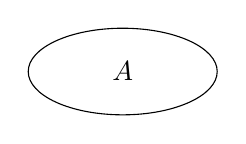
\begin{tikzpicture}
\draw (0,0) ellipse (1.2 and 0.55);
\node at (0,0) {$A$};
\end{tikzpicture}
\end{adjustbox}
\end{center}
graduir. ignored

$\bigoplus\Omega_{2n}^U(X)$ and $\bigoplus\Omega_{2n+1}^U(X)$ —

— from graduir. (ост. забывает)

\underline{Theor.} [Под заголовком, в маленькой рамке: Morava and Quillen.]

$\exists$ \Unclear{GELFAND-P000442}{theorem-prefix}{пл./мн.} откр. в топ. Зар. мн-во [вставлено, обведено: в] $A$, такое что

слой в $\forall$ точке есть гр. $K^\bullet(X)$ $(=K^0(X){}$
\Unclear{GELFAND-P000442}{sum-full}{Между K⁰(X) и K¹(X) плотный обведённый бинарный знак; предположительно ⊕, возможно ⊗.}
$K^1(X))$ !!

$\mathbb Z[t_0,\ldots,t_n,\ldots][t_1^{-1}]$ — это и есть то самое откр. мн-во.

[Над $P_1$, под первым $t_0$: отдельный U/ψ-подобный нисходящий знак; непрерывная стрелка от $t_1$ не установлена.]
$t_1=P_1$ — compl. proj. bundle.
\Unclear{GELFAND-P000442}{projective-mark}{Над P₁ под первым t₀ имеется отдельный U/ψ-подобный нисходящий знак без непрерывного стержня от t₁. Справа сверху от P₁ отдельный восходящий наклонный штрих, возможно прим.}

[Разделительная черта с промежутком.]

$R$ — commutative;

$\Gamma(R)=\left\{\sum_{i=1}^{\infty}a_it^i\mid a_i\in R\right\}$,

$a_1\in R^*$ [стрелка вниз: обрат.]

гр. отн. композиции отобр.

\SourcePage{GELFAND-P000443}{68}
$\Gamma(R)$ — inf. dim alg. group. (compos. — polynomial).

\underline{$\Gamma$ acts on $A$.}

Sheaf $\Omega_*^U$ is an equivariant sheaf (const on orbits).

$\Gamma:\{\text{Rings}\}\longrightarrow\{\text{groups}\}$.
\SourceFigure{GELFAND-P000443}{functor-connector}{Справа явный наконечник; слева маленький открытый угловой/крючковый конец, его роль не определена.}

Наст. теор. должна сост. в опис. орбит.

[Зачёркнуто:
\Incomplete{GELFAND-P000443}{fiber-full}{В отменённой записи различимы O-подобная петля, соединённые r/b-подобные следы и точка; Orb.-подобный кандидат частичен, скрытые буквы и целое старое слово не восстановлены.}]
over $D$ — fibers $K^\bullet(X)$.

$D_{(p,h)}\quad p\text{ prime};\quad1<h<\infty,\quad h\in\mathbb Z$ — orbits.

[Справа за двумя вертикальными чертами:] орбиты.

$D_\infty=\text{fibers }H^*(X,\mathbb Z)$.

[Разделительная черта с промежутком.]

$K(h)$ — functor $K(h)^{\Unclear{GELFAND-P000443}{k-degree}{*}}(X,\mathbb Z_p)$ — $\mathbb Z_p$-module.

Bott periodicity in dim $2(p^h-1)$.

$\exists$ Adams oper.
\begin{center}
\begin{adjustbox}{max width=\linewidth}
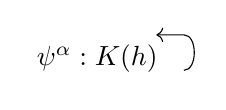
\begin{tikzpicture}
\node at (0,0) {$\psi^\alpha:K(h)$};
\draw[->] (1.1,-0.15) to[out=0,in=0] (1.1,0.3) -- (0.75,0.3);
\end{tikzpicture}
\end{adjustbox}
\end{center}

\Unclear{GELFAND-P000443}{division-units}{Буква перед ∈ похожа на α, возможно λ; фраза: «units of p-adic division algebra of ranke h²».}

This is station. subgroup of a point on the orbit.

\underline{След. раз — продолжение.}

[Слева в круге: \Unclear{GELFAND-P000443}{circled-margin}{угловой петлевидный знак а/q/? с нисходящим крючком и отдельной точкой; верх круга наведён}.]

\underline{Формальные группы}

$A$ — пр-во модулей для 1-мерных коммут. форм. групп.

$F$ — форм. гр. над кольцом $R$, если зад. элем.
\Unclear{GELFAND-P000443}{formal-ring-full}{Запись F∈R, затем два левых скобочных знака, X,Y и два правых; внутренний левый знак C-подобен. Предположительно F∈R[[X,Y]], возможно буквально R[C X,Y]].}

1) $F(X,Y)=F(Y,X)$;

2) $F(0,X)=X$;

3) $F(X,F(Y,Z))=F(F(X,Y),Z)$.

(обр. есть автоматически).

$X,Y$ — форм. перем. — буквы.

\SourcePage{GELFAND-P000444}{unlabelled}
\underline{$f\in\Gamma(R)$} $\Rightarrow$

[Под правым концом подчёркивания наклонная черта, рядом:
\Unclear{GELFAND-P000444}{top-side-mark}{Маленькая s-подобная буква со штрихом справа сверху; возможно s′ или 5 со штрихом.}]

$f=a_1t+a_2t^2+\ldots$.

$a_1\in R^*$.

Замена перем. —

$F^f(X,Y)=f^{-1}\Unclear{GELFAND-P000444}{formula-delimiter}{[}F(f(X),f(Y))$.
[Под формулой открытая сверху скобка: нижняя горизонталь и два вертикальных конца.]

$f$ действ. на мн-ве форм. групп.

$R$ — кольцо $\rightsquigarrow\{\text{форм. группы }A(R)\text{ — мн-во.}\}$

$A:(\text{Rings})\overset{\text{Functor}}{\longrightarrow}(\text{Sets})$.

it is representative.

$A(R)\cong\operatorname{Hom}_{(\text{Rings})}(\Omega_u;R)$.
\Unclear{GELFAND-P000444}{omega-full}{В обозначении кольца после Ω нижний u-подобный знак; возможно строчная u или нижняя U. Не превращён в верхнюю U или звёздочку.}

[Под $\Omega_u$, вертикальное равенство:] $\mathbb Z[t_0,t_1,\ldots]$.

$\operatorname{Hom}$ опр. знач. на $t_i$. какие форм. гр.

[Зачёркнуто:
\Incomplete{GELFAND-P000444}{cancelled-line}{Предположительно начальные ∀R-подобные знаки и позднее C-подобная запись; длинная отменённая строка закрыта горизонтальной чертой и петлями, целиком не восстановлена.}]

$\forall R:\quad\Gamma(R)\times A(R)\longrightarrow A(R)$;

$\Gamma\times A\longrightarrow A$.

($\Gamma$ действ. на $A$ как алг. гр. на алг. мн-зии).

$A(R)\underset{\mathrm{def}}{=}\operatorname{Hom}(\Omega_u,R)$.

$\Gamma$ — форм.
\Unclear{GELFAND-P000444}{substitutions-word}{Предположительно «подстановки»; в соединённых средних буквах нерегулярные штрихи.}

[Стрелка вверх от $\Gamma(R)$ к $f$; подпись:]
$f$ —
\Unclear{GELFAND-P000444}{f-caption-full}{Подпись после f — допускает «подст.», «индив.» или «модиф.»; округлый средний след и пересечённые конечные штрихи остаются неоднозначными.}

[Стрелка вверх от первого нижнего $A(R)$ к $F$; подпись:] $F$ — форм. группа.

$\Gamma(R)\times A(R)\longrightarrow A(R)$.
\Unclear{GELFAND-P000444}{bottom-old}{Первое нижнее A переписано плотными штрихами; нынешняя A-подобная буква различима, прежний слой не определён.}

$(f,F)\longrightarrow F^f$.
\SourcePage{GELFAND-P000445}{69}
\underline{Каждан.}

$\mathbb Z[t_0,t_1,\ldots]$ и форм. группа
\Incomplete{GELFAND-P000445}{formal-cancel}{Зачёркнутое короткое слово перед «над R» не восстановлено.}
над $R$.

$\Vert$\quad \underline{\underline{$R$ — кольцо хар. $0$.}}

\underline{\underline{$\Omega$.}}

Постр. инвар. диффер. на форм. группе — однозн. опр.
\begin{equation*}
\underline{\omega=\sum \Unclear{GELFAND-P000445}{coefficient-case}{c_i}\Unclear{GELFAND-P000445}{omega-symbols}{x}^{i}\,d\Unclear{GELFAND-P000445}{omega-symbols}{x};}
\end{equation*}
\underline{Отобр.:}\quad $t_i\longrightarrow \underline{\Unclear{GELFAND-P000445}{coefficient-case}{c_i}}\in R$.

Получ. отобр. $\Omega\longrightarrow R$. [Волнистое подчёркивание.]

\medskip
\underline{14/IV}\quad \underline{\underline{И.М.Гельфанд.}}

\underline{О докл. Дайсона}\quad \underline{«Неосуществлённые возможности».}

[На правом поле: Анекдот про тоннель.]

Цель: убедить мат. и физ., как много они потеряли из-за того,
что не слушали друг друга.

\underline{Пример 1.}\quad \underline{(развлеч. Дайсона)}
\begin{equation*}
\Unclear{GELFAND-P000445}{eta-product}{\prod_{m=1}^{\infty}(1-x^m)^{24}}=\eta^{24}(x)
=\sum_{n=1}^{\infty}\tau(n)x^n
\quad\text{(ф-я Рамануджана)}
\end{equation*}
Тождество: [Волнистое подчёркивание.]
\begin{equation*}
\tau(n)=
\sum_{\substack{
 a,b,c,d,e\equiv1,2,3,4,5\ (\mathrm{mod}\,5)\\
 a+b+c+d+e=0\\
 a^2+b^2+c^2+d^2+e^2=10n}}
\frac{(a-b)(a-c)(a-d)(a-e)(b-c)(b-d)(b-e)(c-d)(c-e)(d-e)}
{1!\,2!\,3!\,4!}.
\end{equation*}
$\eta(x)$ — ф-я Дедекинда.

\underline{Другой физик-любитель}.
аналог. ср-му $\eta^{10}(x)$.

Дайсон: для $\eta^d(x)$,\quad
$d=3,8,10,14,15,21,24,26,28,35,36$.

[От $3$ стрелка вниз к «Якоби»; от $8$ к «Клейн», ниже «Фрике».]

Это размерности простых алгебр Ли.
\begin{equation*}
\begin{array}{ccccccc}
A_1&A_2&Sp(4)&-&-&.&A_4=SL(5)\\
3&8&10&-&-&.&24
\end{array}
\end{equation*}
Произв. — по всем \Unclear{GELFAND-P000445}{roots-terminology}{простым корням (положит.)} гр. $SL(5)$.

\underline{\underline{$26$}} — выпадает — неясно.

\SourcePage{GELFAND-P000446}{unlabelled}
$2.$\quad $c\to0,\ c\to\infty,\ R\to\infty$ — пред. переходы
в кинем. \Unclear{GELFAND-P000446}{kinematic-word}{группе}.

\underline{\underline{Morava.}}

\underline{Кириллов (повторение).}

$X\longrightarrow\Omega_n(X)$ — группа,\quad $\Omega_n(*)$ — модуль.

[Зачёркнуто: \Unclear{GELFAND-P000446}{triple-cancel}{Тройка.}]
\quad $(M,\xi,\alpha,f)$

$(M,\xi,\alpha)$ — слабо компл. мн-зие
\begin{equation*}
\left(
\Unclear{GELFAND-P000446}{alpha-cancel}{\text{зачёркнутый знак}}\quad
\underbrace{\tau(M)+[k]=\xi+[k']}_{\alpha},
\quad \xi\text{ — уже компл. расслоение}
\right)
\end{equation*}
$\alpha$ — фиксир. разложение.

$f:M\longrightarrow X$.

Отнош. эквивал. [Волнистое подчёркивание.]

\SourceFigure{GELFAND-P000446}{bordism-figure}{Слева цилиндр с двумя овальными торцами, M и N под ними, $w$ под серединой; над торцами и серединой три треугольника с подписями $\xi,\Sigma,\eta$. Справа круг с горизонтальной штриховкой и X рядом. К нему направлены верхняя стрелка с g, средняя с F и нижняя с f. Подпись f находится над $t_2$ следующей строки. Вверху справа отдельный цилиндр с двумя стрелками внутрь от торцов. Точное соединение стрелок с торцами и роль отдельного цилиндра не восстановлены.}

\underline{Теорема.}\quad $\Omega_*(*)=\mathbb Z[t_1,t_2,\ldots]$,\quad
$\operatorname{deg} t_i=2i$.

$t_1\leftrightarrow CP^1$.

[Разделитель: две черты и точка.]

\underline{$A$ — кольцо коборд. точки $\Omega_*(*)$.}

\underline{$M$ — модуль над $A$}\quad $(\Omega_*(X))$.

\underline{$\operatorname{Spec} A=\Unclear{GELFAND-P000446}{spec-glyph}{\mathbb A}$.}

$M$ опр. \underline{пучок} над
\underline{$\Unclear{GELFAND-P000446}{spec-glyph}{\mathbb A}$}.

[Справа: Описание $M_x$? $(x\in \Unclear{GELFAND-P000446}{fiber-base}{M})$; \underline{\underline{слой пучка}}.]

$\Unclear{GELFAND-P000446}{spec-glyph}{\mathbb A}$ имеет точки $3$-х типов.

\SourcePage{GELFAND-P000447}{70}
\Unclear{GELFAND-P000447}{opening-words}{Важна траект.} точки под действием беск. группы.

\underline{\underline{Орбиты:}}

$1)$ одна откр. плотная — общ. полож.

$2)$ одна замкн.

$3)$ сч. число \Unclear{GELFAND-P000447}{orbit-word}{промежут.} орбит

$1)$ слой $K(X)$. (в $\forall$ точке) (откр. плотн.)

$2)$ $p,n$ ($p$ — простое, $n$ — натур.)
\quad $K^{\Unclear{GELFAND-P000447}{k-sup-cancel}{\text{зачёркнутые }n,p}}(n)(X,\mathbb Z_p)$.
— новый хар. пр-ва $X$. [Фраза «пр-ва X» охвачена снизу скобкой.]

$3)$ $H^*(X,\mathbb Z)$ в $\forall$ точке.

[Разделитель: две черты и точка.]

\underline{\underline{Уточнение:}}

$(a_1,\ldots,a_n,\ldots)\in A$

[Слева: max ид.]

$J=(t_1-a_1,\ldots,t_n-a_n,\ldots)A\subset A$.

\underline{$M/MJ$} — вект. пр-во (точнее $A/J$ — модуль).

[Слева: это. Зачёркнуто: это растёт над. Под «над» вписано: растёт.]
точкой \underline{\underline{$J$}}.

\underline{Разбиение $A$ на куски.}

\Incomplete{GELFAND-P000447}{a-title-cancel}{Зачёркнутая строка: начальное A и конечное «форм.» читаются; закрытая промежуточная часть не восстановлена.}

$G$ — гр. форм. замен переменных.

$W_1$ — алг. форм. вект. полей

$W'_1$ — действ. алг. \Unclear{GELFAND-P000447}{differentials-word}{дифференциалов}.

[Справа от этих двух строк вертикальная двойная черта и запись:]
\begin{equation*}
g:x\longrightarrow a_1x+a_2x^2+a_3x^3+\ldots
\end{equation*}
$a_i\in\mathbb Z$ и обратимо $(a_1=1)$.

Можно $\forall$ кольца. — в частности из $A$.

\underline{$(a_1$ — обр. эл. кольца$)$}

\underline{Форм. $1$-мерн. группа:}
\begin{equation*}
x*y=x+y+\alpha xy+\beta x^2y+\delta xy^2+\ldots
\quad(\alpha,\beta\in\text{кольцу})
\end{equation*}
Ассоциативность — \underline{ед. треб.}

Они эквив., если один зак. умн. $\longrightarrow$ другой форм. заменой
пер. $\Unclear{GELFAND-P000447}{coordinate-symbol}{\psi}(x)=\lambda_1x+\lambda_2x^2+\ldots$,\quad
$\lambda_1$ — обр. эл. кольца.
\begin{equation*}
F_1(x,y)=\Unclear{GELFAND-P000447}{coordinate-symbol}{\varphi}^{-1}\bigl(F_2(\Unclear{GELFAND-P000447}{coordinate-symbol}{\psi}(x),\Unclear{GELFAND-P000447}{coordinate-symbol}{\psi}(y))\bigr)
\end{equation*}
[На правом поле, за двойной чертой: Это \Unclear{GELFAND-P000447}{isomorphic-word}{изоморф.} группы.]

\SourcePage{GELFAND-P000448}{unlabelled}
\underline{\underline{Теор.}}

Над Полем хар. $0$ — [В пузыре над следующими словами: $1$-мерн.]
форм. гр. $\sim$ сложению \underline{\underline{$x+y$}}!

Коммут. выводится.

Опис. с пом. форм. дифф.

[Стрелка вниз от этого места к следующему «Док-во».]

\underline{\underline{Док-во:}}
\begin{equation*}
\varphi^{-1}=\int\frac{dx}{f},\quad
\text{где }\underline{f(x)=\frac{\partial F}{\partial y}(x,0)}.
\end{equation*}
(простая проверка).

Не хар. $0$ — интегралы не сущ.

$\displaystyle\int x^{p-1}\,dx$ не сущ. над полем хар. $p$.
\begin{equation*}
\Unclear{GELFAND-P000448}{second-inverse}{\varphi}^{-1}
=\int a\,dx=\int\frac{dx}{f}
\end{equation*}
\underline{$a\,dx$} — форм. дифф.,
[зачёркнуто: \Unclear{GELFAND-P000448}{reconstruct-cancel}{восстан.}]
опр. группу
\begin{equation*}
a(x)=1+a_1x+a_2x^2+\ldots
\end{equation*}
\underline{Действие группы (в дифф.)}
\begin{equation*}
a(x)\longrightarrow a(\Unclear{GELFAND-P000448}{action-symbol}{\psi}(x))\Unclear{GELFAND-P000448}{action-symbol}{\psi}'(x)
\end{equation*}
\underline{\underline{$a(x)$ — любой ряд.}} Ему ств. форм. группа
(теорема о сущ. унив. группы)

\underline{\underline{Morava.}}
\begin{equation*}
a(x)=1+\underset{[CP(1)]}{\underline{\underline{a_1}}}x+
\underset{[CP(2)]}{a_2}x^2+\ldots
\quad\text{— предл. Кириллова}
\end{equation*}
(теор. Мищенко —
\Incomplete{GELFAND-P000448}{mishchenko-cancel}{После тире зачёркнут целый короткий фрагмент; текст не восстановлен.}
здесь получ. $CP(n)$.

\underline{Теорема:}\quad $G$ — групп. схема.\quad $X_{\Unclear{GELFAND-P000448}{scheme-x-mark}{\text{знак}}}$ — $G$-схема (над $\mathbb Z$).

Пусть $\Unclear{GELFAND-P000448}{k-first-cancel}{\text{зачёркнутый }K}$
гладко, $G$ плоско и всё нётерово

$\Unclear{GELFAND-P000448}{k-all-cancel}{\text{зачёркнутый знак}}\quad
K$ (алг. замкн. поле) и $G(k)$ действ. транзитивно на $X(k)$

\SourcePage{GELFAND-P000449}{71}
$\exists S\subset G$\quad $X\cong G/S$.

[От $S$ короткая стрелка вниз: подгр. (стабилиз.).]

[Ряд разделительных точек. Остальная часть кадра пустая.]

\SourcePage{GELFAND-P000450}{unlabelled}
\underline{\underline{25/IX–72г.}}\quad \underline{\underline{Габриэлов.}}

Сем-во структур Ходжа над $S$ (\Unclear{GELFAND-P000450}{non-singular-word}{неособе} аналит. мн-зие)

$1)$ $\mathcal H_{\mathbb Z}$ — лок. своб. пучок $\mathbb Z$-модулей конечн. типа.

[Зачёркнуто: $2)$.] По нему стр. лок. трив. компл. рассл. $H_C$.

\begin{equation*}
H_C=H_{\mathbb Z}\otimes_{\mathbb Z}C,\quad
H_O=H_{\mathbb Z}\otimes_{\mathbb Z}O_S
\end{equation*}
и $H_R$ — вещ. расслоение

[От $H_C$ стрелка вправо вниз: лок. система (Делинь) — рассл. со связностью; снизу длинная скобка.]

$2)$ в $H_C$ убывающая фильтрация голом. расслоениями
\begin{equation*}
H_C=F^0\supset F^1\supset\ldots\supset F^n
\end{equation*}

$3)$ в $H_O$ [вписано в пузыре: есть] естеств. связность (Гаусса—Манина)
\begin{equation*}
\nabla:H_O\longrightarrow\Omega^1\otimes_{O_S}H_O
\end{equation*}
[Справа: (дифф. опер. с ядром. — сеч. $H_C$).]

(есть лок. пост. сечения
$\Unclear{GELFAND-P000450}{local-section-glyph}{\mathbb Z}$ —
образ пучка $H_C$)

Связность должна удовл. условию
\begin{equation*}
\nabla(\mathcal F^p)\subset\Omega_S^1\otimes\mathcal F^{p-1}
\quad(\mathcal F^p=F^p\otimes_C O_S)
\end{equation*}

$4)$ $\psi$ — билин., лок. пост. форма на $H_C$, дающая при
огранич. на $\forall$ слой настоящую структ. Ходжа.

[Разделитель: две черты и точка.]

Классифицир. пр-во структур Ходжа

Рассм. [Ниже разделитель: две черты и точка.]
\begin{equation*}
F=\{F^0\supset F^1\supset\ldots\supset F^n\}
\quad\text{— флаги }\underline{\text{фиксир. разм.}}
\end{equation*}
в фикс. пр-ве, $C^n$ ($\dim$ могут быть с пропусками).

[На правом поле за двойной чертой: набор $\dim$ — задаётся.]

[Разделитель: две черты и точка.]

$D$ — пр-во;

Точки пр-ва
$\Unclear{GELFAND-P000450}{point-cancel}{\text{зачёркнутый знак}}$ —
\underline{флаги}.

Берём лин. пр-во $H_C$ с билин. формой $\psi(x,y)$
(невырожд.; кос. либо симм.)

$\bar D$ — мн-зие всех флагов [зачёркнуто: \Unclear{GELFAND-P000450}{bottom-cancellation}{знак}] в $H_C$ с фикс. набором $\dim$

\SourcePage{GELFAND-P000451}{72}
$\Unclear{GELFAND-P000451}{initial-cancel}{\text{зачёркнутый знак}}$
с условием $1)$ $\psi(F^p,F^{\Unclear{GELFAND-P000451}{orthogonality-exponent}{n-p}})=0$.

Это алгебраич. подмн-зие $\bar D$.

$\psi$ либо симм., либо кососимметрич. (\underline{\underline{def}}).

$2)$ $F^p\oplus\bar F^{n-p+1}\cong H_C$.

$H_{\mathbb Z}\subset H_R\subset H_C$\quad \underline{\underline{тоже задано}}

По невыр. флагу опр. градуировка и автом. Вейля
\begin{equation*}
H^{p,n-p}=F^p\cap\bar F^{n-p}
\end{equation*}
Автом. Вейля:
\begin{equation*}
C\xi=i^{2p-n}\xi\quad\text{при }\xi\in H^{p,n-p}
\end{equation*}
Эти усл. выделяют в $\bar D$ откр. подмн-зие $D$.

\Incomplete{GELFAND-P000451}{condition-cancel}{Перед «Ещё условие» зачёркнуто целое слово; оно не восстановлено.}
Ещё условие:\quad $\psi(x,C\bar x)>0$ при $x\ne0$.

Определим на $D$ структуру однор. пр-ва.

$G$ — группа всех вещ. преобр. $H_R$, сохр. $\psi$
$\{\psi(gx,gy)=\psi(x,y)\}$.

Тогда $G$ действует на $D$. [Волнистое подчёркивание.]

\underline{Теорема:}
$1)$ [Перед $G$: \Unclear{GELFAND-P000451}{theorem-insert}{яв. и зачёркнутый знак};
над ним пузырь со вставкой $1$.] $G$ действ. транзитивно

$2)$ ст. Подгруппа $H$ (сохр. флаг.) компактна.

\underline{Док-во:} из явного вычисления $G$ и $H$.

$K\subset G$ — макс. комп. подгруппа.

$G/H\longrightarrow G/K$\quad оно не голоморфно.

В $G/K$ есть компл. структура

\SourcePage{GELFAND-P000452}{unlabelled}
\Incomplete{GELFAND-P000452}{title-cancel}{Верхний подчёркнутый заголовок полностью перекрыт многократным зачёркиванием; текст не восстановлен.}

[Разделитель: две черты и точка.]

\underline{$1$-я лекция Манина о $p$-адич. числах!} (пересказ)

$K$ — лок. поле,
\Incomplete{GELFAND-P000452}{k-cancel}{После «лок. поле» зачёркнут короткий фрагмент в скобке; текст не восстановлен.}

(кон. расш. $p$-адич. чисел)

[Зачёркнуто в скобках:
\Incomplete{GELFAND-P000452}{parent-cancel-full}{В двухстрочной зачёркнутой скобке различаются разрозненные «форм.», «степ.» и «ряд…»; полный текст и закрытые слова не восстановлены.}.]

$A$ — кольцо целых,\quad $m\subset A$.

[От $m$ стрелка вниз: макс. идеал.]

$P^1(K)$ — проект. прямая.

\begin{equation*}
G=\text{дв-ния её}=
\left\{z\longrightarrow\frac{az+b}{cz+d}\mid a,b,c,d\in K,\ \det\ne0\right\}
=GL(2,K)/K^*
\end{equation*}
$U\subset G$;\quad $U=GL(2,A)/A^*$.

Постр. $G/U$ — граф $\Delta$ — аналог плоск. Лобачевского.

\underline{Опр.:} Решётка в $K^2$ — своб. $A$-модуль с $2$-мя образ.
\begin{equation*}
L=Ae_1\oplus Ae_2.
\end{equation*}
\underline{Лемма.} Если $L_1$ и $L_2$ — $2$ реш., то $\exists$ базис $e_1,e_2$
в $K^2$, такой, что
\begin{gather*}
L_1=Ae_1\oplus Ae_2;\\
L_2=m^{\nu_1}e_1\oplus m^{\nu_2}e_2
=A\pi^{\nu_1}e_1\oplus A\pi^{\nu_2}e_2
\end{gather*}
($\pi$ — образующая
$\Unclear{GELFAND-P000452}{ideal-symbol-tight}{\text{неразборчивый знак}}$
макс. идеала)

(аналог. теор. лин. алг. об одновр. приведении)

[Справа скобка и $\nu_1,\nu_2\in\mathbb Z$.]

\underline{Def.}\quad $L_1\sim L_2$, если $L_1=\alpha L_2$, где $\alpha\in K^*$.

Есть аналог расстояния — как в симм. пр-вах.
$\Unclear{GELFAND-P000452}{sim-margin-cancel}{\text{зачёркнутый знак}}$
— см. \underline{А.Вейль}.

[Разделитель: две черты и точка.]

Вершины графа $\Delta^{(0)}$
$\Unclear{GELFAND-P000452}{dimension-glyph}{\text{зачёркнутый знак}}$
— классы экв. решёток

$G$ действ. на $\Delta^{(0)}$.

\SourcePage{GELFAND-P000453}{73}
$\Lambda_1=\{L_1\},\ \Lambda_2=\{L_2\}$ — классы решёток.

[Над $L_1$ стрелка к $\Delta^{(0)}$.]

[В рамке: $L_2\subset L_1$.]

[На правом поле за двойной чертой: $A/m=k=F_q$.]

\begin{gather*}
L_1=Ae_1\oplus Ae_2\\
L_2=Ae_1\oplus A\pi^\nu e_2
\end{gather*}
— так выбир. \Unclear{GELFAND-P000453}{representative-word}{представителя},\quad \underline{$\nu\ge0$}.

$\nu$ наз. расстоянием\quad \underline{\underline{$\nu=d(\Lambda_1,\Lambda_2)$}}.

[В рамке:]
$L_1/L_2=$
\Incomplete{GELFAND-P000453}{quotient-cancel}{Зачёркнутый фрагмент между равенством и A/m в формуле фактора не восстановлен.}
$A/m^\nu$.

\underline{Теор.} Это корр. опр. и есть \underline{расстояние}.

\underline{\underline{Вариант:}}
\begin{equation*}
L_1/L_2\cong A/\pi^{\nu_1}A\oplus A/\pi^{\nu_2}A
\end{equation*}
\begin{equation*}
d(\Lambda_1,\Lambda_2)=|\nu_1-\nu_2|
\end{equation*}
$\Lambda_1,\Lambda_2$ — соседи в $\Unclear{GELFAND-P000453}{neighbor-notation}{\Lambda^0}$, если
$d(\Unclear{GELFAND-P000453}{neighbor-notation}{\Lambda'},\Lambda^2)=1$.

Соед. их ребром. Получим граф $\Delta$.

\underline{Теорема:}\quad $\Delta$ — дерево (св. граф без циклов),
причём из $\forall$ верш. вых. точно $q+1$ ребро.

$\Delta$ и есть плоск. Лобач. — действует $G$ и т.д.

\SourceFigure{GELFAND-P000453}{disk-figure}{Внизу овальная граница с небольшим разрывом у верхнего правого края. Внутри несколько длинных и вложенных коротких дуг, нижние дуги сходятся у границы. Цепочка закрашенных узлов идёт слева через середину вправо, затем вверх к верхнему краю; у левого узла есть короткая петлеобразная ветвь, вверху справа — тонкие ответвления. У нижней левой дуги бледная подпись, похожая на 0 или O. Точные соединения линий у верхнего правого края, смысл пересечений дуг с цепочкой и число узлов там не установлены.}

[Нижний разделитель: две черты и точка.]

\SourcePage{GELFAND-P000454}{unlabelled}
\underline{\underline{Д. Каждан}}\quad
Ст. Тэйта, Математика, \underline{$13:2$, §$3$}.

(о поле $C_p$ — пополнение алг. замык. $\bar Q_p$ \Unclear{GELFAND-P000454}{q-p-link-word}{или}
$Q_p$ — $p$-адич. чисел)

[Разделитель: две черты и точка.]

$K$ — конечн. расш. поля $Q_p$.

$O_K$ — целые в $K$.

[Под $O_K$ \Unclear{GELFAND-P000454}{vertical-ring}{вертикальный U-образный знак}, ниже $m_K$ — макс. идеал; под $m_K$ два коротких вертикальных штриха повтора, затем $(\pi)$.]

$k=O_K/m_K$.

$L$ — конечн. расш. $K$,
$\Unclear{GELFAND-P000454}{ol-cancel}{\text{зачёркнутая формула}}$
$O_L$ — целые в нём.

$m_L=(\tau)$,\quad $\ell=O_L/m_L$,

$G=\operatorname{Gal}(L:K)$.

Введ. фильтрацию в $G$ и док., что $G$ разрешимо.

На $L$ и $K$ —
$\Unclear{GELFAND-P000454}{norm-cancel}{\text{зачёркнутый знак}}$
зададим норму, так что $|\pi|=(\operatorname{Card}k)^{-1}$

\underline{\underline{Def.}}
\Incomplete{GELFAND-P000454}{def-cancel}{После Def зачёркнуто целое короткое слово; оно не восстановлено.}
\begin{equation*}
g\in G_i\Longleftrightarrow
\forall x\in O_L\quad x^g-x\in m_L^i
\end{equation*}
\begin{equation*}
G=G_0\supset G_1\supset\ldots\supset G_n=\{e\}.
\end{equation*}
$G_i$ — норм. делитель в $G$.

\underline{Теорема:}\quad $G_i/G_{i+1}$ — аб. группа

\underline{$1)\ i=0$.}\quad
$G\overset{\varphi}{\longrightarrow}\operatorname{Gal}(\ell:k)$
(естеств. отобр.)

\underline{Построение $\varphi$:}\quad $\bar x\in\ell,\ g\in G$

$x\in \Unclear{GELFAND-P000454}{residue-representative}{L}$
\begin{equation*}
\bar x^g\overset{\mathrm{def}}{=}\overline{x^g}
\end{equation*}
$g\in\ker\varphi\Longleftrightarrow\Unclear{GELFAND-P000454}{kernel-quantifier}{\bar x\in\ell},\ \bar x^g=\bar x$,
т.е. $\bar x^g-\bar x=0$, т.е.
% UNACCEPTED joint source-review r2 draft; local baseline reconciled with the original human return.
% Bracketed placement notes describe source ink and are editorial.
\SourcePage{GELFAND-P000455}{74}

\Unclear{GELFAND-P000455}{top-old-fragment}{Зачёркнуто: т.е.?}
\Incomplete{GELFAND-P000455}{top-cancelled}{Остальная зачёркнутая запись в верхнем левом углу не восстановлена.}

$x^g-x\in\mathfrak m_L$, т.е. $g\in G_1$.
\begin{equation*}
0\longrightarrow G_0/G_1\overset{\varphi}{\longrightarrow}\operatorname{Gal}(\ell:k)
\end{equation*}
\underline{Упражнение:} $\varphi$ — изоморфизм.

2) $G_1/G_2$ — \Unclear{GELFAND-P000455}{quotient-question}{$?$}

$G_1$ \Unclear{GELFAND-P000455}{ramification-label}{$\overset{\psi_1}{\longrightarrow}$} $\ell^*$
\begin{equation*}
g\sim\!\longrightarrow\overline{\tau^g/\tau}\qquad\text{(не зав. от выб. }\tau\text{)}
\end{equation*}
Ядро \Unclear{GELFAND-P000455}{kernel-pronoun}{его?} есть $G_2$.
\begin{equation*}
G_i/G_{i+1}\longrightarrow\ell^+\quad\text{(аддит. группа поля }\ell\text{).}
\end{equation*}
$g$ \Unclear{GELFAND-P000455}{higher-label}{$\overset{\psi_i}{\longrightarrow}$}
$\displaystyle\overline{\left(\frac{\tau^g/\tau-1}{\tau^{i-1}}\right)}$.

\underline{Теор.} $G_{i+1}=\operatorname{Ker}\psi_i$.
\Unclear{GELFAND-P000455}{kernel-domain}{Сохранены написанные область $G_i/G_{i+1}$ и равенство $G_{i+1}=\operatorname{Ker}\psi_i$; уточнение области и диапазона $i$ здесь не дано.}

$G_1$ наз. подгруппой инерции гр. Галуа.

Неразветвлённое расширение $\underset{\mathrm{def}}{\Leftrightarrow}$ $G_1=\{e\}$;

\Unclear{GELFAND-P000455}{weak-word}{слаборазветвл.} $G_2=\{e\}$;

чисто разветвлённым $G_0=G_1$.

\begin{center}\rule{25mm}{0.3pt}\quad$\cdot$\quad\rule{35mm}{0.3pt}\end{center}

\SourcePage{GELFAND-P000456}{unlabelled}

\underline{Семинар будет начинаться в $18^{\underline{00}}$.}

\noindent \underline{\underline{2/X-72г.}}\qquad \underline{А. Габриэлов.}

$S$ — компл. аналит. мн-зие.

$H_Z$ — лок. своб. $Z$-пучок

($Z$ — пост. пучок; сечение над св. обл. — пост. целое число;
$H_Z$ — лок. своб. пучок $Z$-модулей.
\Unclear{GELFAND-P000456}{modules-old}{Знак с наложенными штрихами: Я.? / $\mathcal F$? / скобка?}
У $\forall$ точки $\exists$ окр.,
у к-рой он изом. $Z\oplus\cdots\oplus Z$).

\Unclear{GELFAND-P000456}{start-old-fragment}{Зачёркнуто: $H$?}
\Incomplete{GELFAND-P000456}{start-cancelled}{Остальная короткая зачёркнутая запись перед скобкой не восстановлена.}
($Z$-пучок, ассоц. с предпучком, к-рый
\Incomplete{GELFAND-P000456}{presheaf-full-cancel}{Две соседние зачёркнутые записи после «к-рый» не восстановлены.}
[Ниже вписано: $F(U)=Z$]).

Пр-во лок. связно $\Rightarrow$ слой $=Z$.

Пр-во пучка $Z$ гомеом. $S\times Z$.

Лок. $H_Z|_U\cong U\times Z^n$.

$\Gamma(U,H_Z)\cong Z^n$.

$S$ связно $\Rightarrow n$ всюду одно.

Покроем окрестностями и фиксир. изоморфизмы над окрестностями
\newline (с точн. до $GL(n,Z)$).

\SourceFigure{GELFAND-P000456}{overlap-sketch}{Два пересекающихся овала: левый шире, правый выше; в общей линзообразной области четыре коротких наклонных штриха. У верхнего левого края есть маленькое угловое окончание, его значение не установлено. Подписей внутри нет.}

ф-и перехода из $GL(n,Z)$.

Можно постр. \underline{лок. трив.} рассл. с такими ф-ями перехода.

Это $H_R$ (или $H_C$ в зависимости от слоя)
\newline [От $H_C$ проведена наклонная черта к подписи:] компл. вект. расслоение

$H_{\mathcal O}$
\Unclear{GELFAND-P000456}{o-old-fragment}{В зачёркнутой формуле: $H$ с индексом?}
\Incomplete{GELFAND-P000456}{o-cancelled}{Остальная формула в прямоугольнике под плотным зачёркиванием не восстановлена.}
\newline [Под $H_{\mathcal O}$, с вертикальной соединительной чертой:]
\underline{пучок голом. сечений $H_C$}

\begin{equation*}
H_{\mathcal O}=H_Z\otimes_Z\mathcal O_S.
\end{equation*}

Имеется естеств. связность (Гаусса-Манина)
\begin{equation*}
\nabla:H_{\mathcal O}\longrightarrow\Omega_S^1\otimes_{\mathcal O_S}H_{\mathcal O}
\quad\text{($C$-лин. гомом.)}
\end{equation*}
$\Omega_S^1$ — голом. дифф. формы пор. $1$.

\SourcePage{GELFAND-P000457}{75}

\underline{опр. связности.}

1. $C$-линейность.

2. $\varphi\in\mathcal O_{S,s}$ (ростки), $f\in H_{\mathcal O,s}\Rightarrow$
\begin{equation*}
\Rightarrow\nabla(\varphi f)=\varphi\nabla f+d\varphi\otimes f.
\end{equation*}

\underline{Наша связность.}

Берём лок. тривиализацию
\newline и базис из пост. сечений (рассл. $H_Z$) $u_i$.
\begin{equation*}
f=\sum\varphi_i u_i,\qquad\varphi_i\in\mathcal O_S.
\end{equation*}
Тогда $\nabla f=\sum d\varphi_i\otimes u_i$.

Это опр. корректно и удовл. всем аксиомам.

Кривизна этой связности равна \Unclear{GELFAND-P000457}{curvature-sign}{$0$?}.

\underline{Требование на связность Г.-М.}
[Справа:] (\underline{или на} \Unclear{GELFAND-P000457}{filter-old}{зачёркнутый знак: $H$? / $F$? / ф?}
\underline{фильтрацию})
\begin{equation*}
\nabla(\mathcal F^p)\subset\Omega_S^1\otimes\mathcal F^{p-1}.
\end{equation*}
\noindent (Гриффитс).

(Задана фильтрация $H_C=F^0\supset F^1\supset\cdots$)
\newline [Под формулой:] голом. подрасслоениями

$\mathcal F^p$ — пучки сечений $F^p$.

\begin{center}\rule{15mm}{0.3pt}\quad$\cdot$\quad\rule{15mm}{0.3pt}\end{center}

[Строка целиком волнисто подчёркнута:] Есть лок. постоянная билин. форма
\Unclear{GELFAND-P000457}{form-letter}{$\psi(x,y)$} на $H_C$.

\Incomplete{GELFAND-P000457}{mid-cancelled}{Короткая зачёркнутая запись перед следующей строкой не восстановлена.}
и в $\forall$ точке $s\in S$ это структура Ходжа.

\begin{center}\rule{15mm}{0.3pt}\quad$\cdot$\quad\rule{15mm}{0.3pt}\end{center}

Пусть $0\le p\le n$, $k_p\ge k_{p+1}$ — послед. чисел.
\begin{equation*}
k_0\ge k_1\ge\cdots\ge k_n.
\end{equation*}
$Z$ — пр-во с элем. $F=\{F^0\supset F^1\supset\cdots\supset F^n\}$,
\newline где \Unclear{GELFAND-P000457}{dimension-sup}{$\dim F^p=k_p$; показатель $p$ переписан.}

Это проект. алг. мн-зие.

\SourcePage{GELFAND-P000458}{unlabelled}

\begin{equation*}
H_C=F^0;\qquad H_Z\subset H_R\subset H_C.
\end{equation*}

Пусть на $H_C$ зад. билин. форма
\Unclear{GELFAND-P000458}{first-form}{$\psi$} (невыр.),
\newline симм. при неч. $n$ и кос. при чётн. $n$; целочисл.
\Unclear{GELFAND-P000458}{parity-statement}{Сохранён порядок рукописи: симм. при неч. $n$ и кос. при чётн. $n$.}

$\overline D$ — подмн. в $Z$ таких флагов, что
\begin{center}
\begin{adjustbox}{max width=\linewidth}
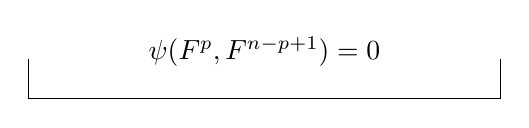
\begin{tikzpicture}
\node at (0,0) {$\psi(F^p,F^{n-p+1})=0$};
\draw (-3,-0.1) -- (-3,-0.6) -- (3,-0.6) -- (3,-0.1);
\end{tikzpicture}
\end{adjustbox}
\end{center}

\noindent\rule{120mm}{0.3pt}

\underline{Доп. усл.}
\newline \underline{на флаги}

1) \Unclear{GELFAND-P000458}{sum-formula}{$F^p\oplus\overline{F^{n-p+1}}\cong H_C$; последний показатель переписан.}

2) По нему стр. градуировка и автом. Вейля $C$
\Unclear{GELFAND-P000458}{weil-link-full}{и?} тогда
\begin{equation*}
\psi(x,C\overline y)\quad\text{полож. опр. эрм. форма на }H_C.
\end{equation*}

Эти условия выделяют $D\subset\overline D$.
\newline [Под $D$:] (открытое).

$D$ наз. классиф. пр-вом структур Ходжа.

Зависит от набора размерностей и формы $\psi$.

\underline{След. раз:} однородность.

гр. компл. пр. $H_C$, сохр. $\psi$, транзит. на $\overline D$

[Слева дописано:] \Unclear{GELFAND-P000458}{real-prefix}{Св. комп. ${}_1$}
гр. вещ. пр. $H_R$, сохр. $\psi$, транзит. на $D$.

\medskip\noindent\rule{120mm}{0.3pt}

\underline{2-я лекция Манина.}

\medskip\noindent\rule{120mm}{0.3pt}

\underline{\underline{\Unclear{GELFAND-P000458}{footer-heading}{Д: Каждан.}}}
Ещё о раб. Тэйта.

\medskip\noindent\rule{120mm}{0.3pt}

\SourceFigure{GELFAND-P000458}{bottom-mark}{Под нижней разделительной чертой слева — узкая высокая петля из нескольких почти вертикальных штрихов, с поперечным штрихом вверху, тёмным узлом внизу и наклонным нижним окончанием. Надёжной буквенной подписи или направления стрелки не установлено.}

\end{document}
